% Template:     Reporte LaTeX
% Documento:    Archivo de ejemplo
% Versión:      3.2.1 (11/03/2023)
% Codificación: UTF-8
%
% Autor: Pablo Pizarro R.
%        pablo@ppizarror.com
%
% Manual template: [https://latex.ppizarror.com/reporte]
% Licencia MIT:    [https://opensource.org/licenses/MIT]

% ------------------------------------------------------------------------------
% NUEVA SECCIÓN
% ------------------------------------------------------------------------------
% Las secciones se inician con \section, si se quiere una sección sin número se
% pueden usar las funciones \sectionanum (sección sin número) o la función
% \sectionanumnoi para crear el mismo título sin numerar y sin aparecer en el índice\begin{document}

\sectionanum{Ejercicios básicos}
Adrián Gaitán: Punto 10 | Tarea 3, Programación II

% SUB-SECCIÓN
% Las sub-secciones se inician con \subsection, si se quiere una sub-sección
% sin número se pueden usar las funciones \subsectionanum (nuevo subtítulo sin
% numeración) o la función \subsectionanumnoi para crear el mismo subtítulo sin
% numerar y sin aparecer en el índice
\subsection{Punto 1}
	
	Ejemplo de pantalla:
 % Please add the following required packages to your document preamble:
% \usepackage{booktabs}
\begin{lstlisting}
Este programa presenta la serie de Fibonacci como la serie que comienza con los dígitos 1 y 0 y va
sumando progresivamente los dos últimos elementos de la serie, así: 0 1 1 2 3 5 8 13 21 34...
Para este programa, se presentará la serie de Fibonacci hasta llegar sin sobrepasar el número 10,000.
0, 1, 1, 2, 3, 5, 8, 13, 21, 34, 55, 89, 144, 233, 377, 610, 987, 1597, 2584, 4181, 6765.
\end{lstlisting}

\begin{lstlisting}
Este programa presenta la serie de Fibonacci como la serie que comienza con los dígitos 1 y 0 y va
sumando progresivamente los dos últimos elementos de la serie, así: 0 1 1 2 3 5 8 13 21 34...
Para este programa, se presentará la serie de Fibonacci hasta llegar sin sobrepasar el número 10,000.
0, 1, 1, 2, 3, 5, 8, 13, 21, 34, 55, 89, 144, 233, 377, 610, 987, 1597, 2584, 4181, 6765.
\end{lstlisting}

\begin{lstlisting}
Este programa presenta la serie de Fibonacci como la serie que comienza con los dígitos 1 y 0 y va
sumando progresivamente los dos últimos elementos de la serie, así: 0 1 1 2 3 5 8 13 21 34...
Para este programa, se presentará la serie de Fibonacci hasta llegar sin sobrepasar el número 10,000.
0, 1, 1, 2, 3, 5, 8, 13, 21, 34, 55, 89, 144, 233, 377, 610, 987, 1597, 2584, 4181, 6765.
\end{lstlisting}

\subsubsectionanum{DFD}
\begin{figure}
  \centering
  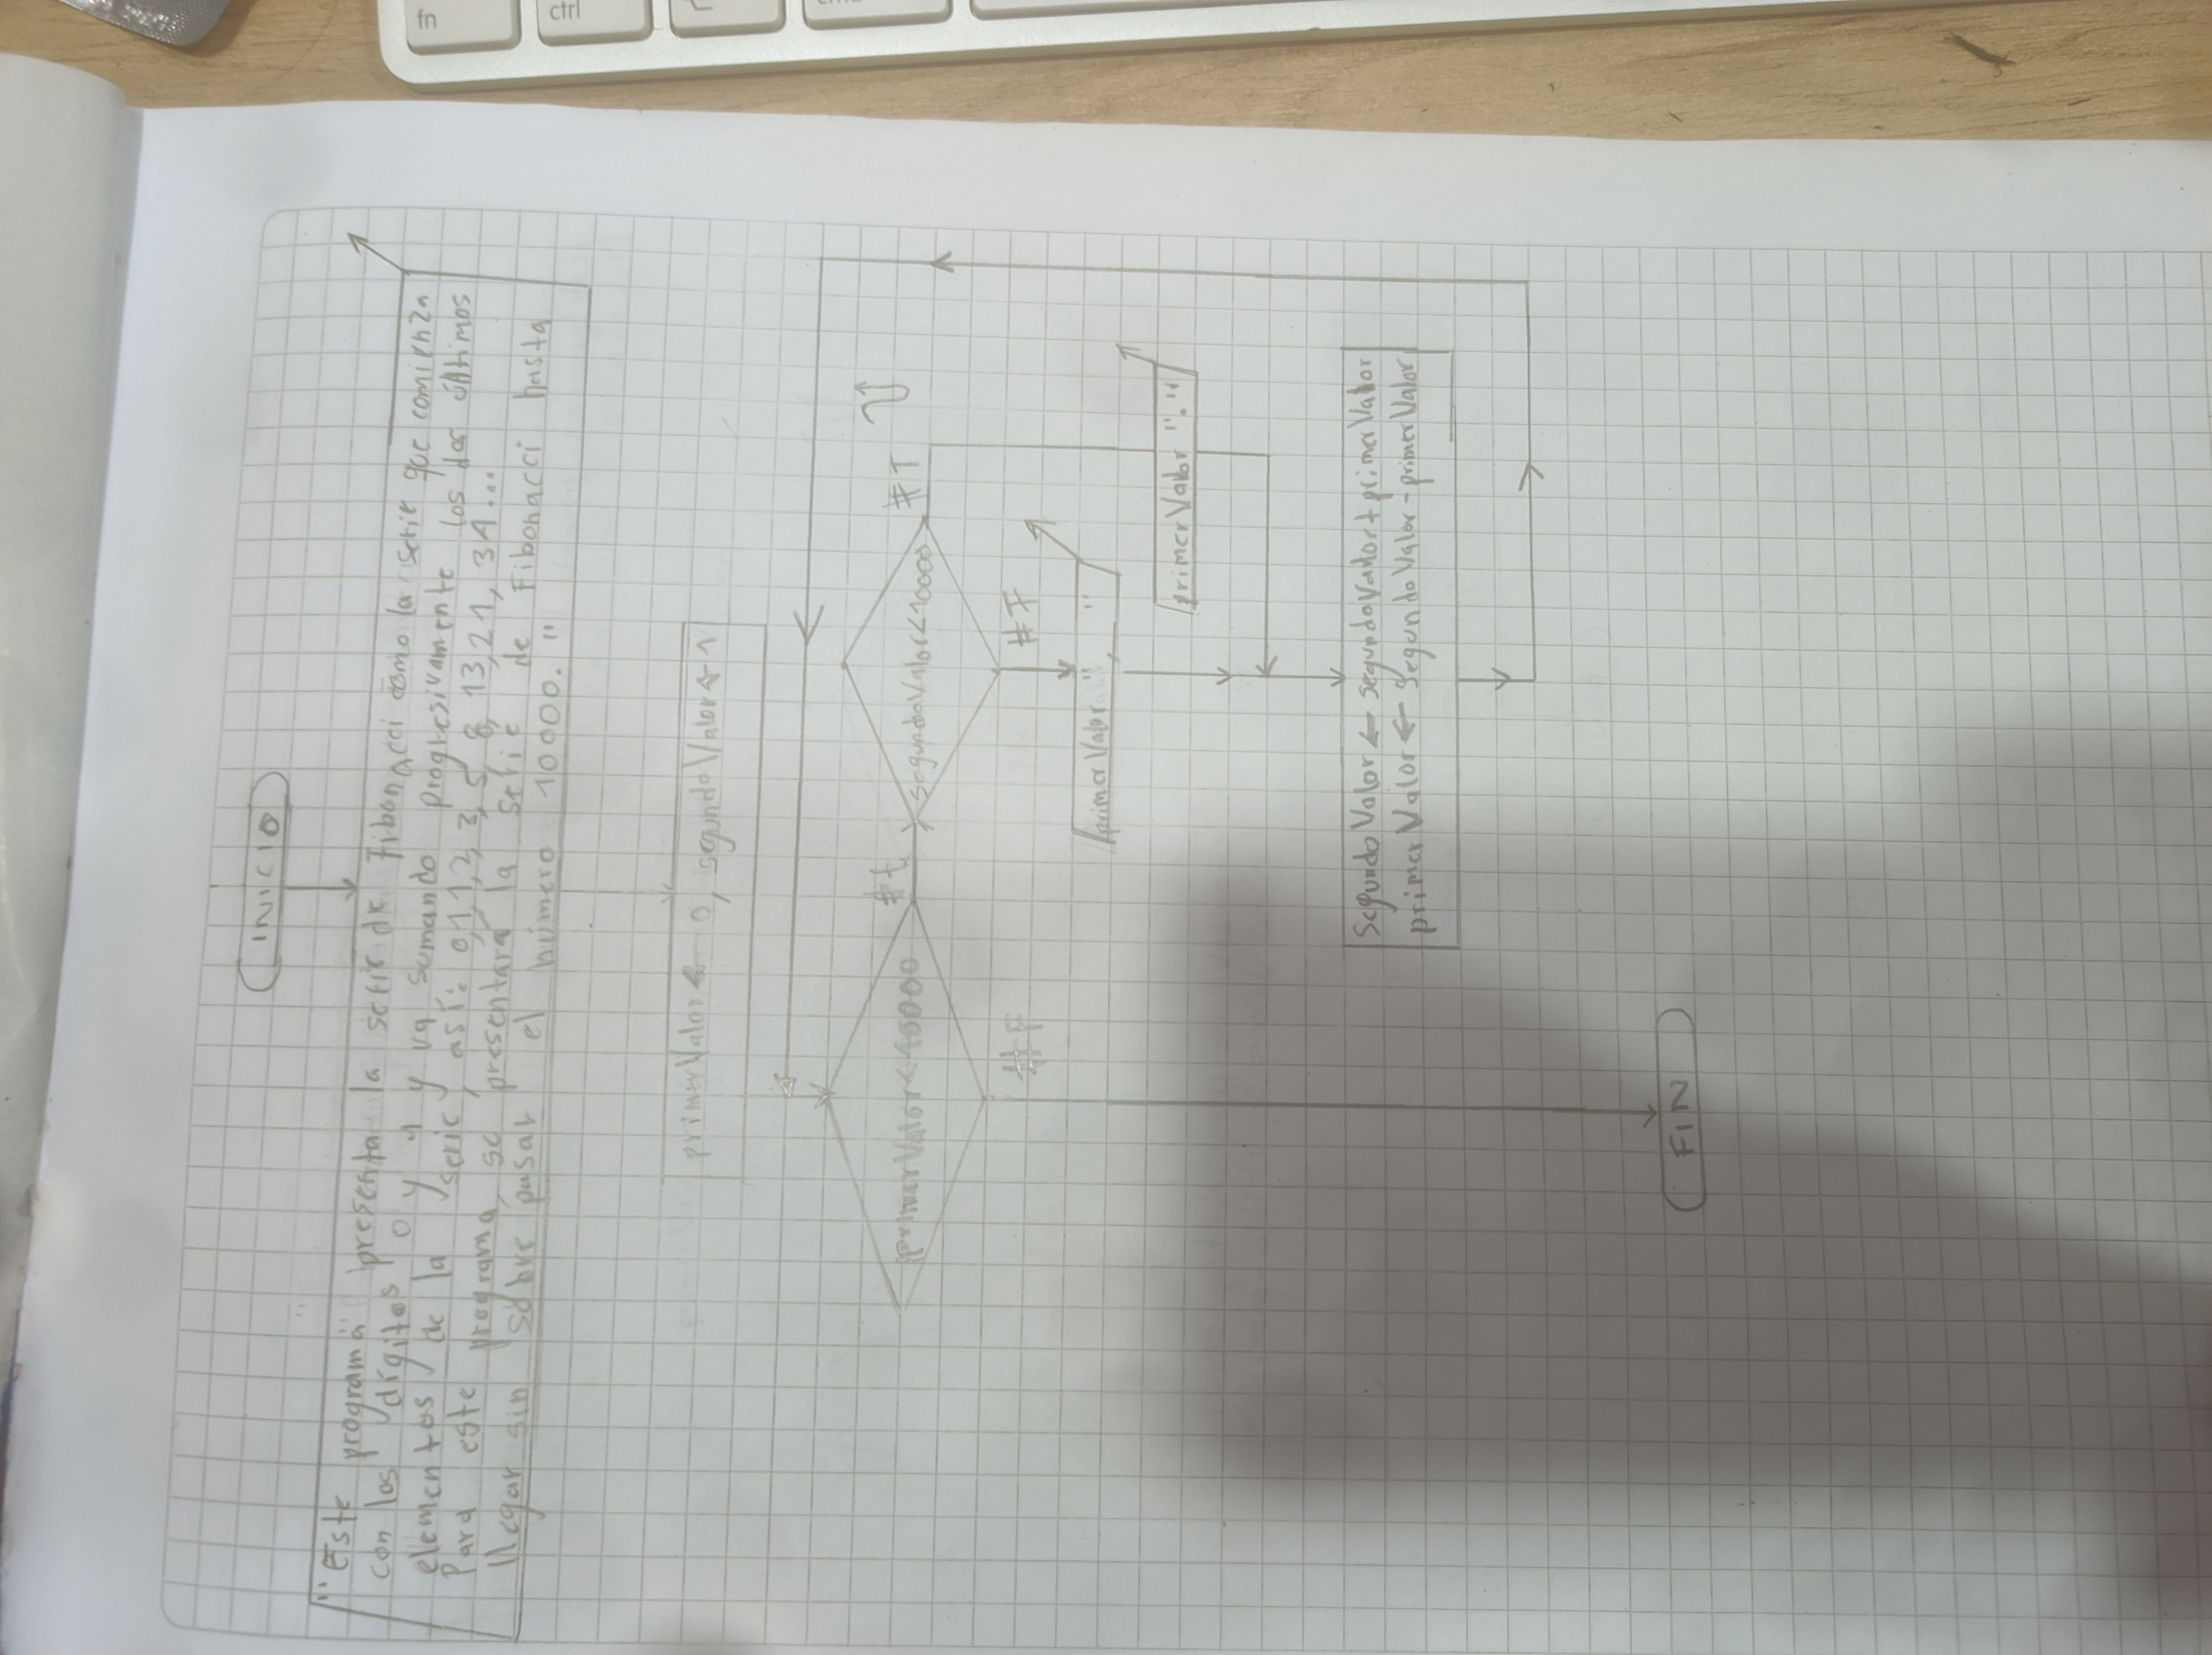
\includegraphics[width=14cm]{dfd/1.jpg}
  \caption{ DFD del punto 1}
  \label{fig: DFD del punto 1}
\end{figure}

\subsubsectionanum{Código}

\importsourcecode[]{c}{code/1.c}{}


\subsection{Punto 2}
	
	Ejemplo de pantalla:
 % Please add the following required packages to your document preamble:
% \usepackage{booktabs}
\begin{lstlisting}
Este programa presenta la suma de los elementos de la serie de Fibonacci entre 0 y 100.
Los números a sumar son: 
0, 1, 1, 2, 3, 5, 8, 13, 21, 34, 55, 89 y su suma es: 232.
\end{lstlisting}

\begin{lstlisting}
Este programa presenta la suma de los elementos de la serie de Fibonacci entre 0 y 100.
Los números a sumar son: 
0, 1, 1, 2, 3, 5, 8, 13, 21, 34, 55, 89 y su suma es: 232.
\end{lstlisting}

\begin{lstlisting}
Este programa presenta la suma de los elementos de la serie de Fibonacci entre 0 y 100.
Los números a sumar son: 
0, 1, 1, 2, 3, 5, 8, 13, 21, 34, 55, 89 y su suma es: 232.
\end{lstlisting}

\subsubsectionanum{DFD}
\begin{figure}
  \centering
  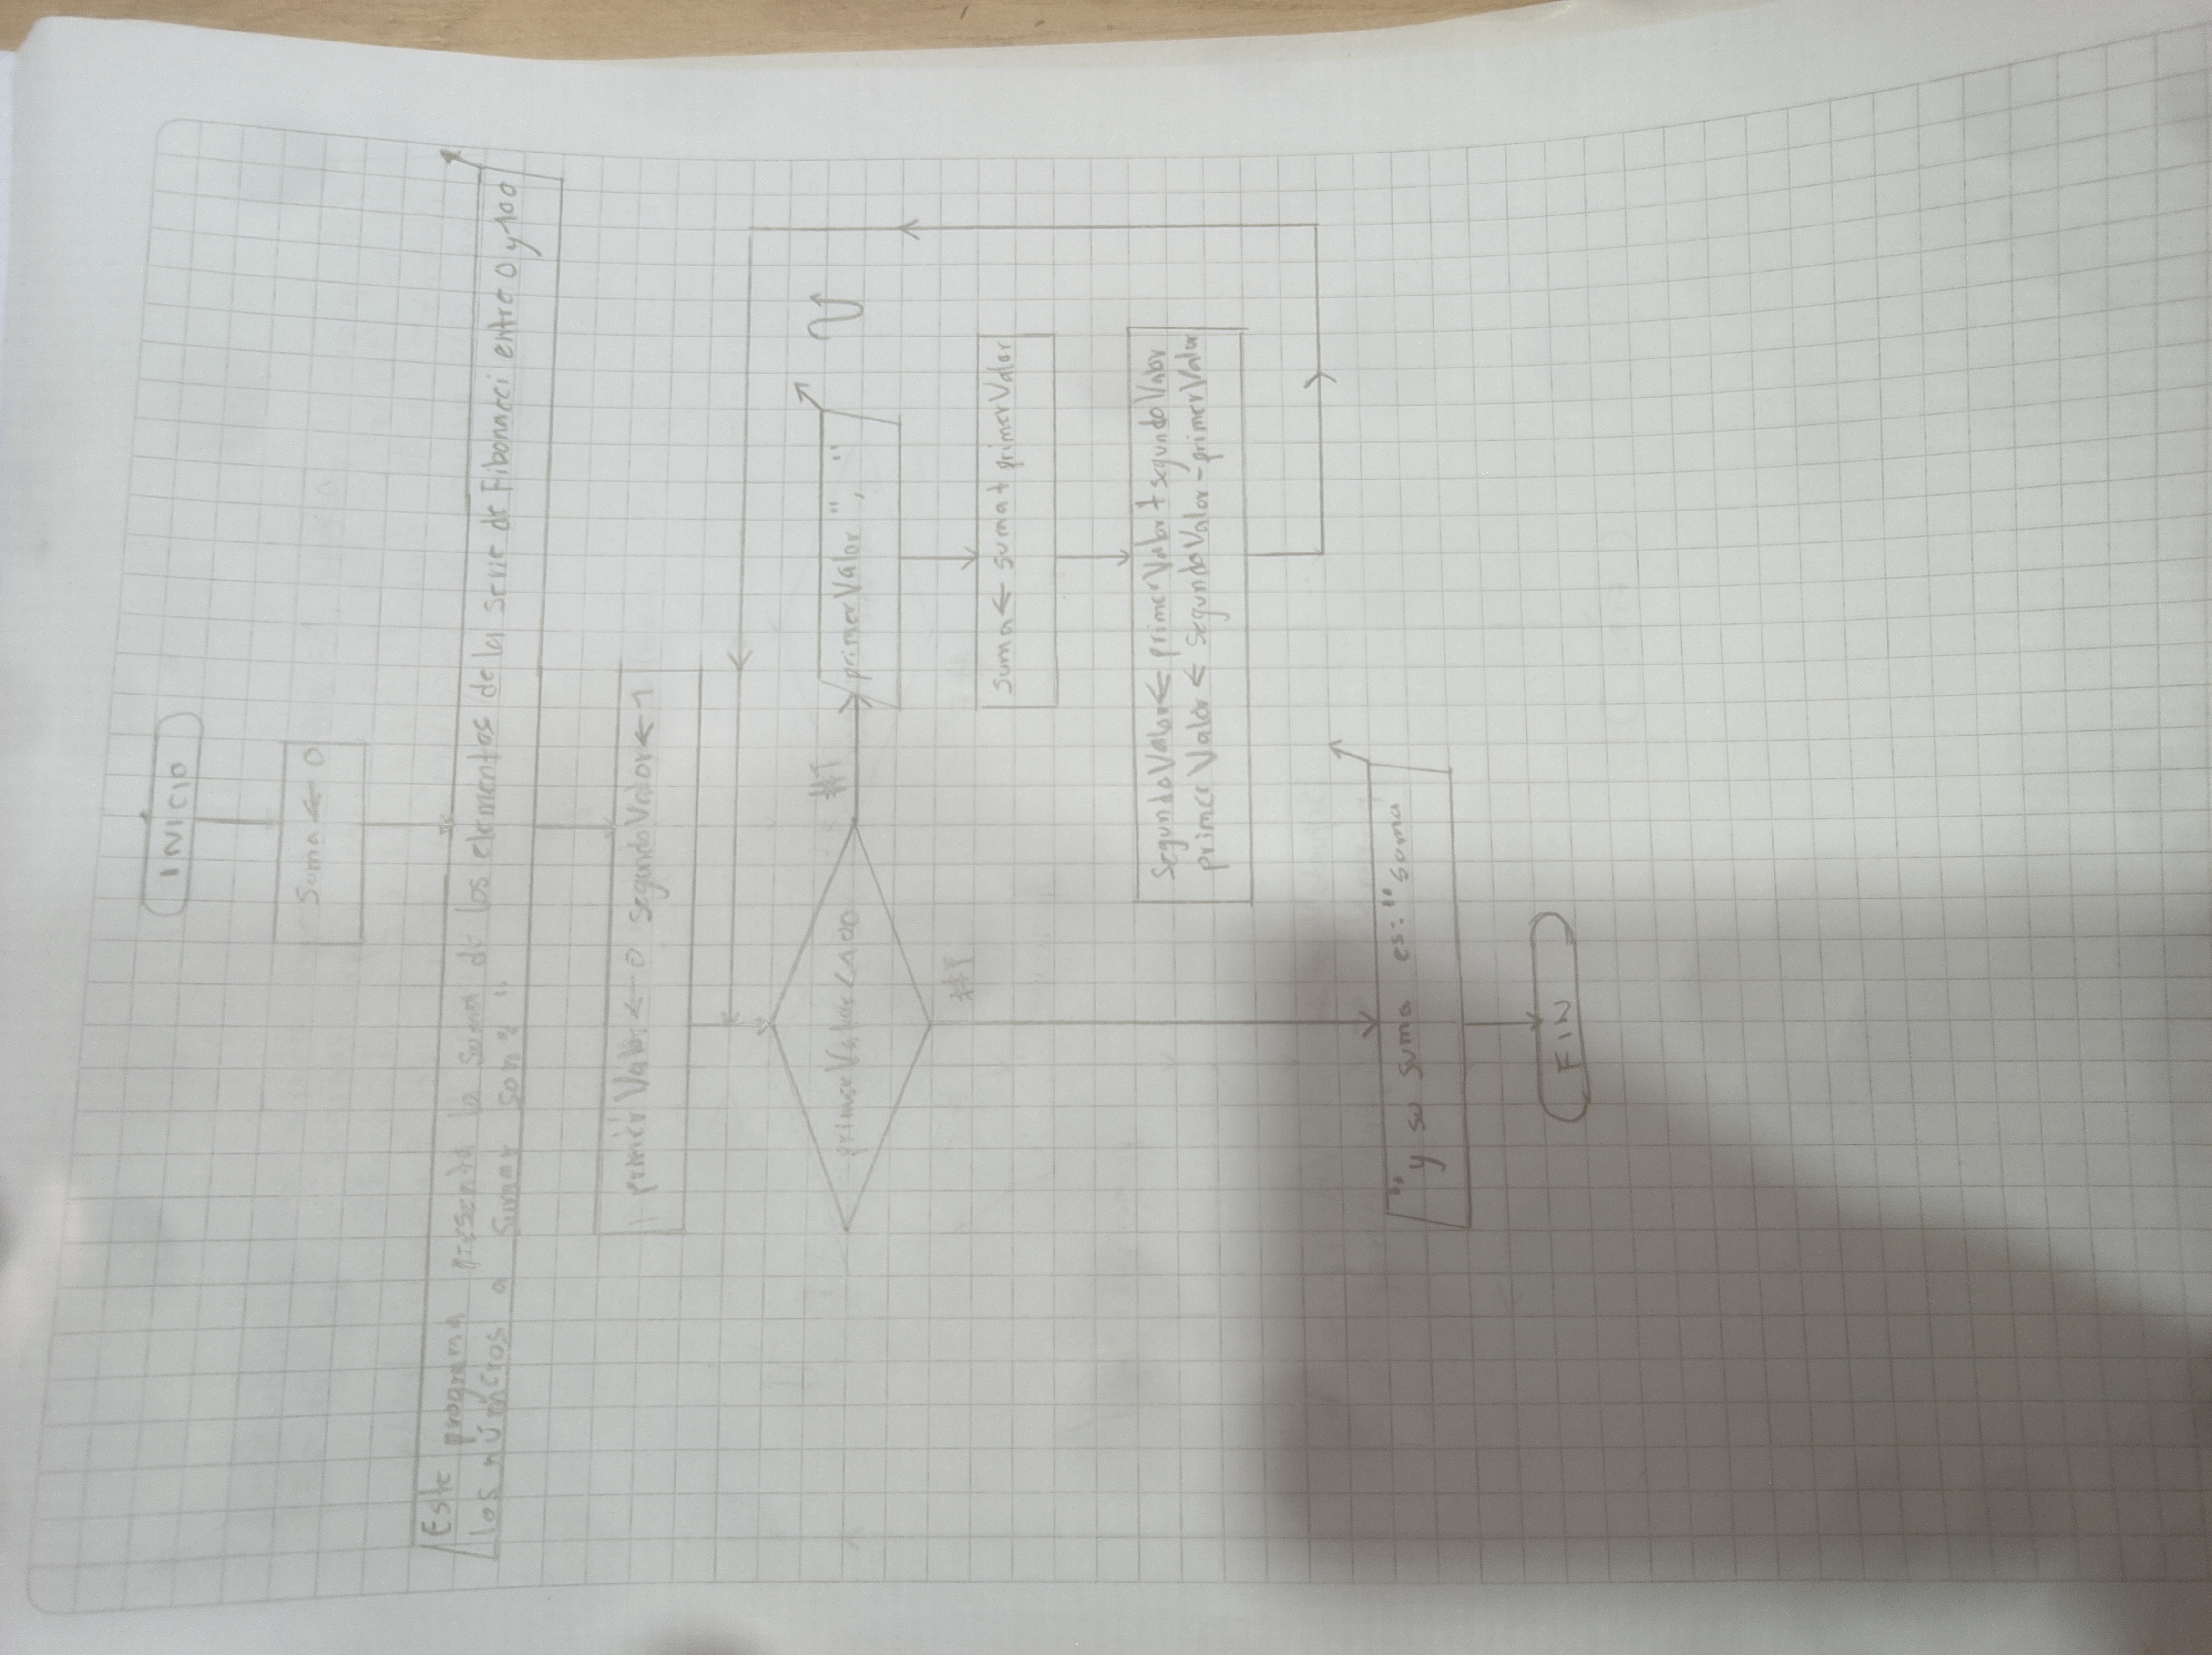
\includegraphics[width=14cm]{dfd/2.jpg}
  \caption{ DFD del punto 2}
  \label{fig: DFD del punto 2}
\end{figure}

\subsubsectionanum{Código}

\importsourcecode[]{c}{code/2.c}{}


\subsection{Punto 3}
	
	Ejemplo de pantalla:
 % Please add the following required packages to your document preamble:
% \usepackage{booktabs}
\begin{lstlisting}
Este programa imprime en pantalla el número de terminos deseados de la serie de Lucas.
Ingrese la cantidad de términos de la serie de Lucas que desea ver: 5

La cantidad 5 de términos de la serie de Lucas son: 2, 1, 3, 4, 7.
\end{lstlisting}

\begin{lstlisting}
Este programa imprime en pantalla el número de terminos deseados de la serie de Lucas.
Ingrese la cantidad de términos de la serie de Lucas que desea ver: 9

La cantidad 9 de términos de la serie de Lucas son: 2, 1, 3, 4, 7, 11, 18, 29, 47.
\end{lstlisting}

\begin{lstlisting}
Este programa imprime en pantalla el número de terminos deseados de la serie de Lucas.
Ingrese la cantidad de términos de la serie de Lucas que desea ver: 20

La cantidad 20 de términos de la serie de Lucas son: 2, 1, 3, 4, 7, 11, 18, 29, 47, 76, 123, 199, 322, 521, 843, 1364, 2207, 3571, 5778, 9349.
\end{lstlisting}

\subsubsectionanum{DFD}
\begin{figure}
  \centering
  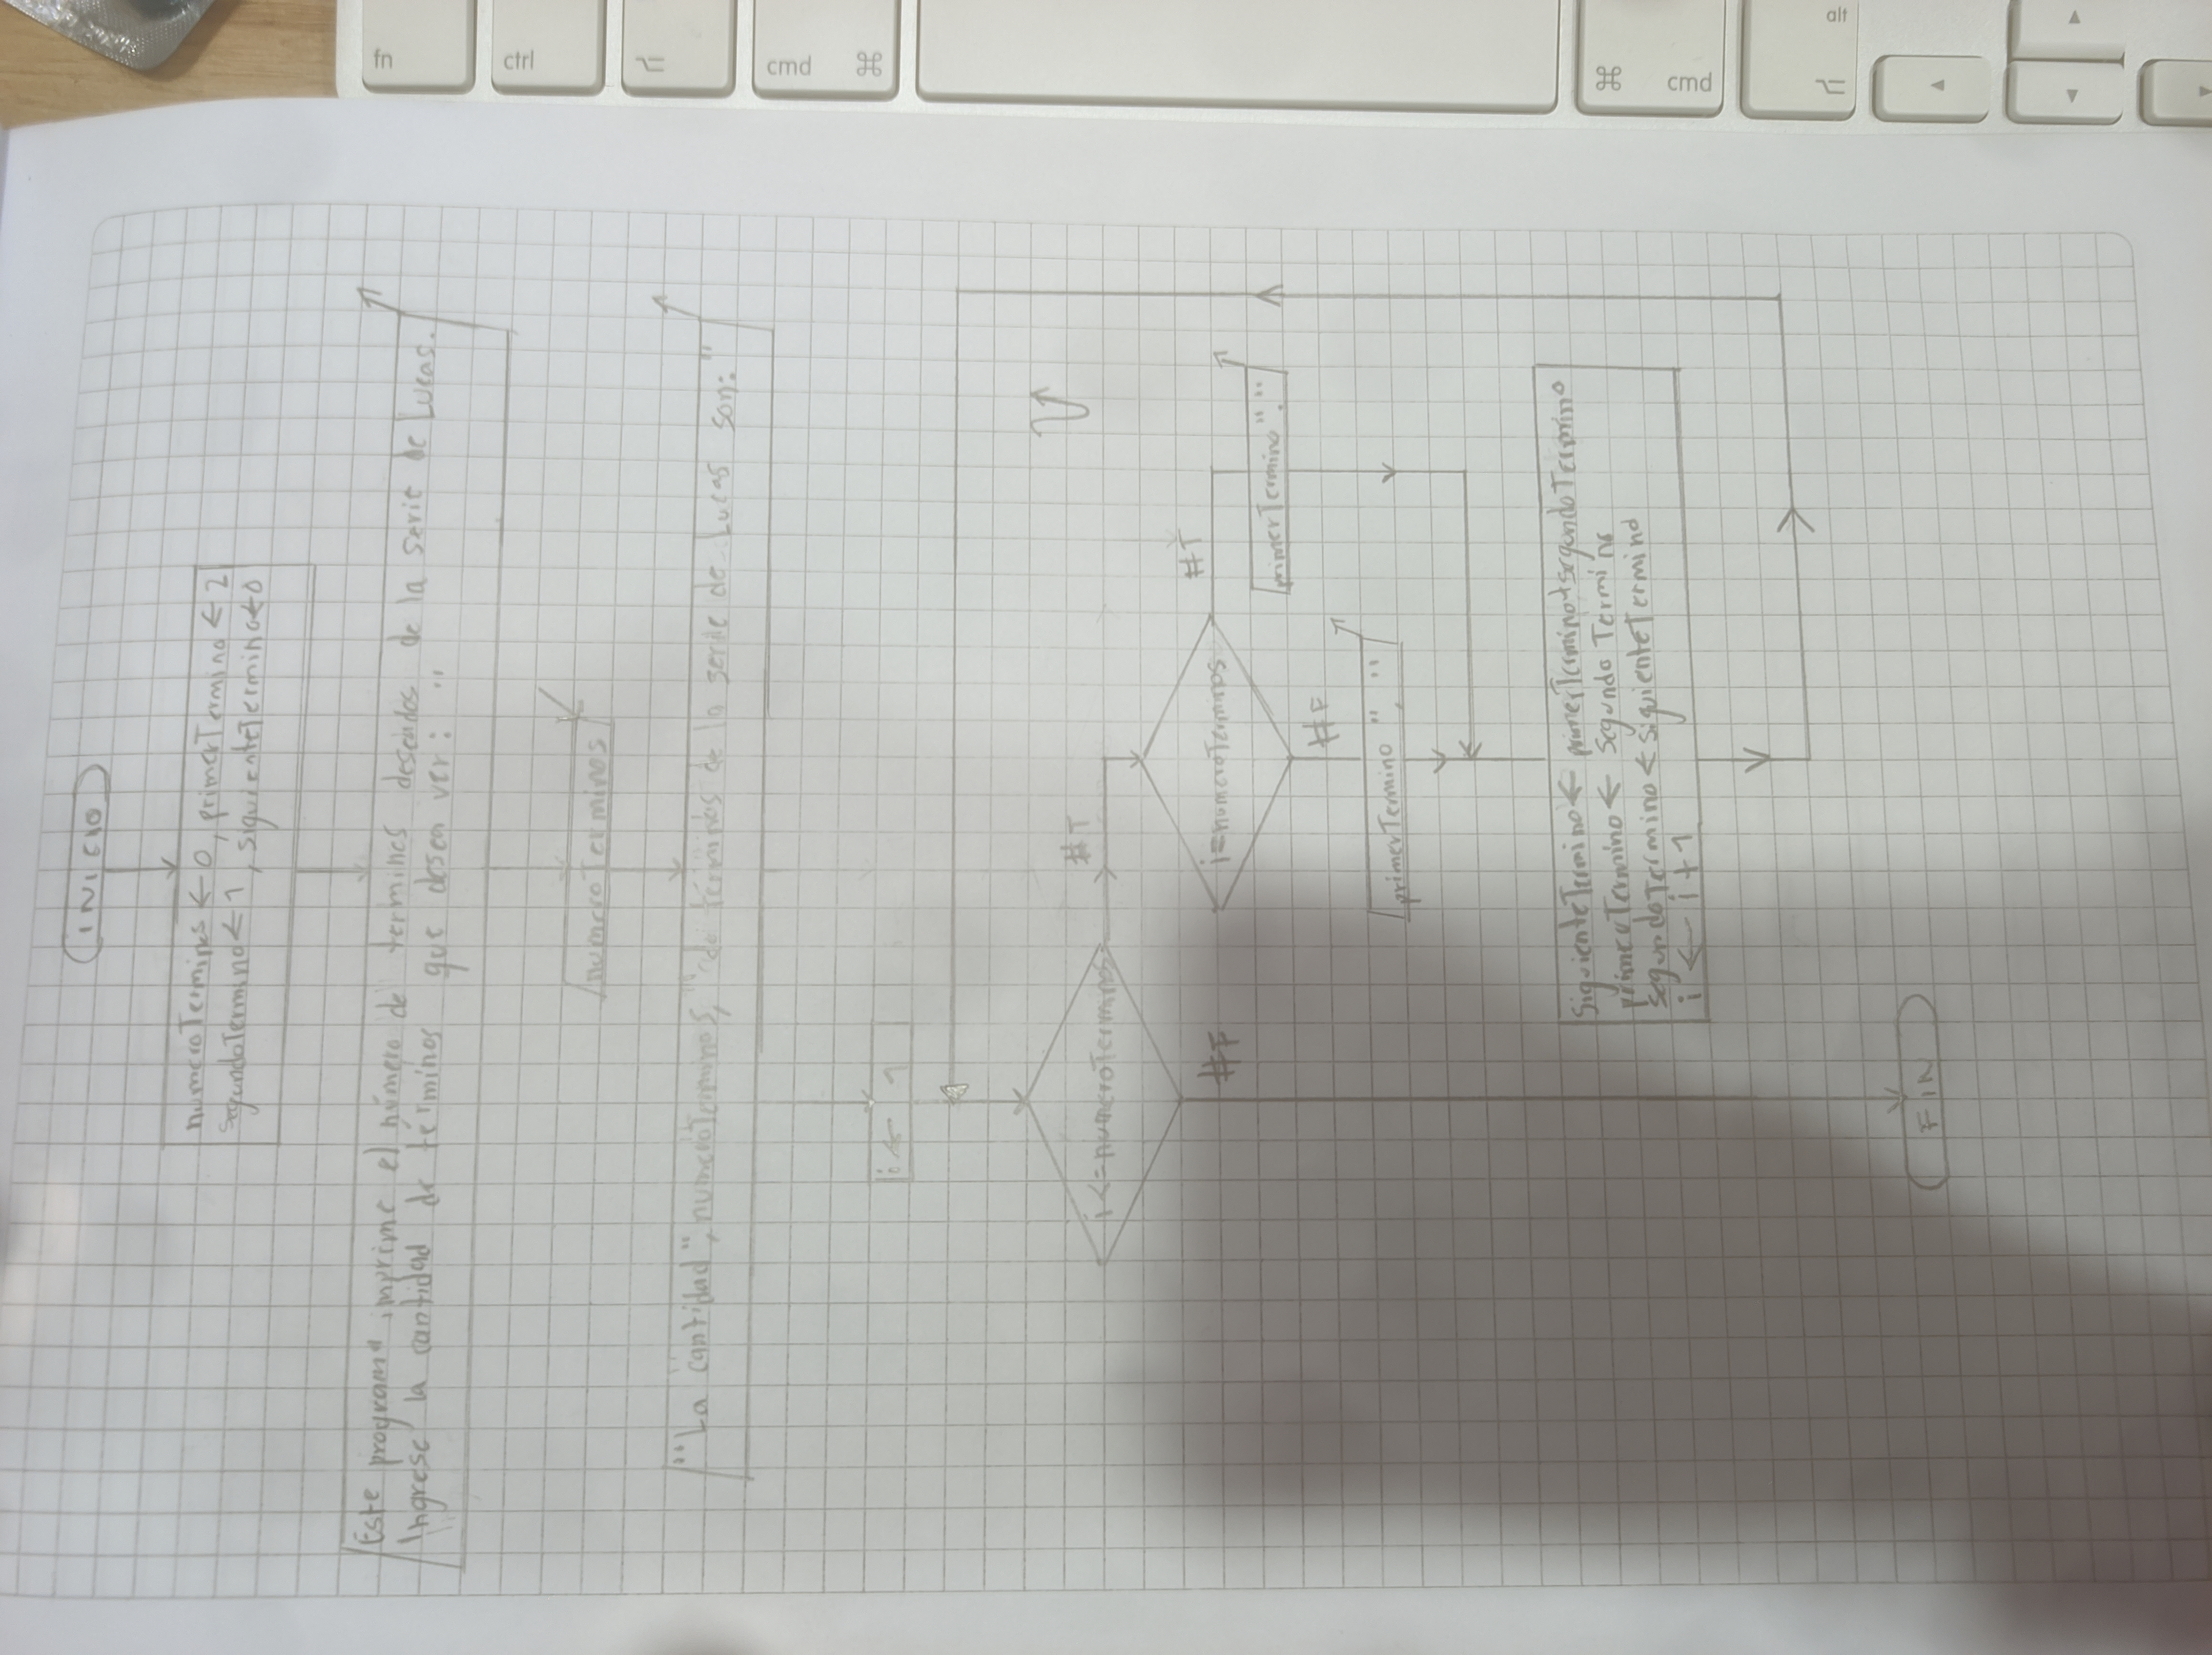
\includegraphics[width=14cm]{dfd/3.jpg}
  \caption{ DFD del punto 3}
  \label{fig: DFD del punto 3}
\end{figure}


\subsubsectionanum{Código}

\importsourcecode[]{c}{code/3.c}{}


\subsection{Punto 4}
	
	Ejemplo de pantalla:
 % Please add the following required packages to your document preamble:
% \usepackage{booktabs}
\begin{lstlisting}
Este programa imprime en pantalla el número de terminos deseados de la serie de Pell.
Ingrese la cantidad de términos de la serie de Pell que desea ver: 4

La cantidad 4 de términos de la serie de Pell es: 0, 1, 2, 5.
\end{lstlisting}

\begin{lstlisting}
Este programa imprime en pantalla el número de terminos deseados de la serie de Pell.
Ingrese la cantidad de términos de la serie de Pell que desea ver: 9

La cantidad 9 de términos de la serie de Pell es: 0, 1, 2, 5, 12, 29, 70, 169, 408.
\end{lstlisting}

\begin{lstlisting}
Este programa imprime en pantalla el número de terminos deseados de la serie de Pell.
Ingrese la cantidad de términos de la serie de Pell que desea ver: 20

La cantidad 20 de términos de la serie de Pell es: 0, 1, 2, 5, 12, 29, 70, 169, 408, 985, 2378, 5741, 13860, 33461, 80782, 195025, 470832, 1136689, 2744210, 6625109.
\end{lstlisting}

\subsubsectionanum{DFD}
% \begin{figure}
%   \centering
%   \includegraphics[width=14cm]{dfd/4.jpg}
%   \caption{ DFD del punto 4}
%   \label{fig: DFD del punto 4}
% \end{figure}

\subsubsectionanum{Código}

\importsourcecode[]{c}{code/4.c}{}


\subsection{Punto 5}
	
	Ejemplo de pantalla:
 % Please add the following required packages to your document preamble:
% \usepackage{booktabs}
\begin{lstlisting}
Este programa imprime en pantalla los primeros n terminos de la serie de Perrin.
Ingrese la cantidad de términos de la serie de Perrin que desea ver: 5

La cantidad 5 de términos de la serie de Perrin son: 3, 0, 2, 3, 2.
\end{lstlisting}

\begin{lstlisting}
Este programa imprime en pantalla los primeros n terminos de la serie de Perrin.
Ingrese la cantidad de términos de la serie de Perrin que desea ver: 9

La cantidad 9 de términos de la serie de Perrin son: 3, 0, 2, 3, 2, 5, 5, 7, 10.
\end{lstlisting}

\begin{lstlisting}
Este programa imprime en pantalla los primeros n terminos de la serie de Perrin.
Ingrese la cantidad de términos de la serie de Perrin que desea ver: 15

La cantidad 15 de términos de la serie de Perrin son: 3, 0, 2, 3, 2, 5, 5, 7, 10, 12, 17, 22, 29, 39, 51.
\end{lstlisting}

\subsubsectionanum{DFD}
\begin{figure}
  \centering
  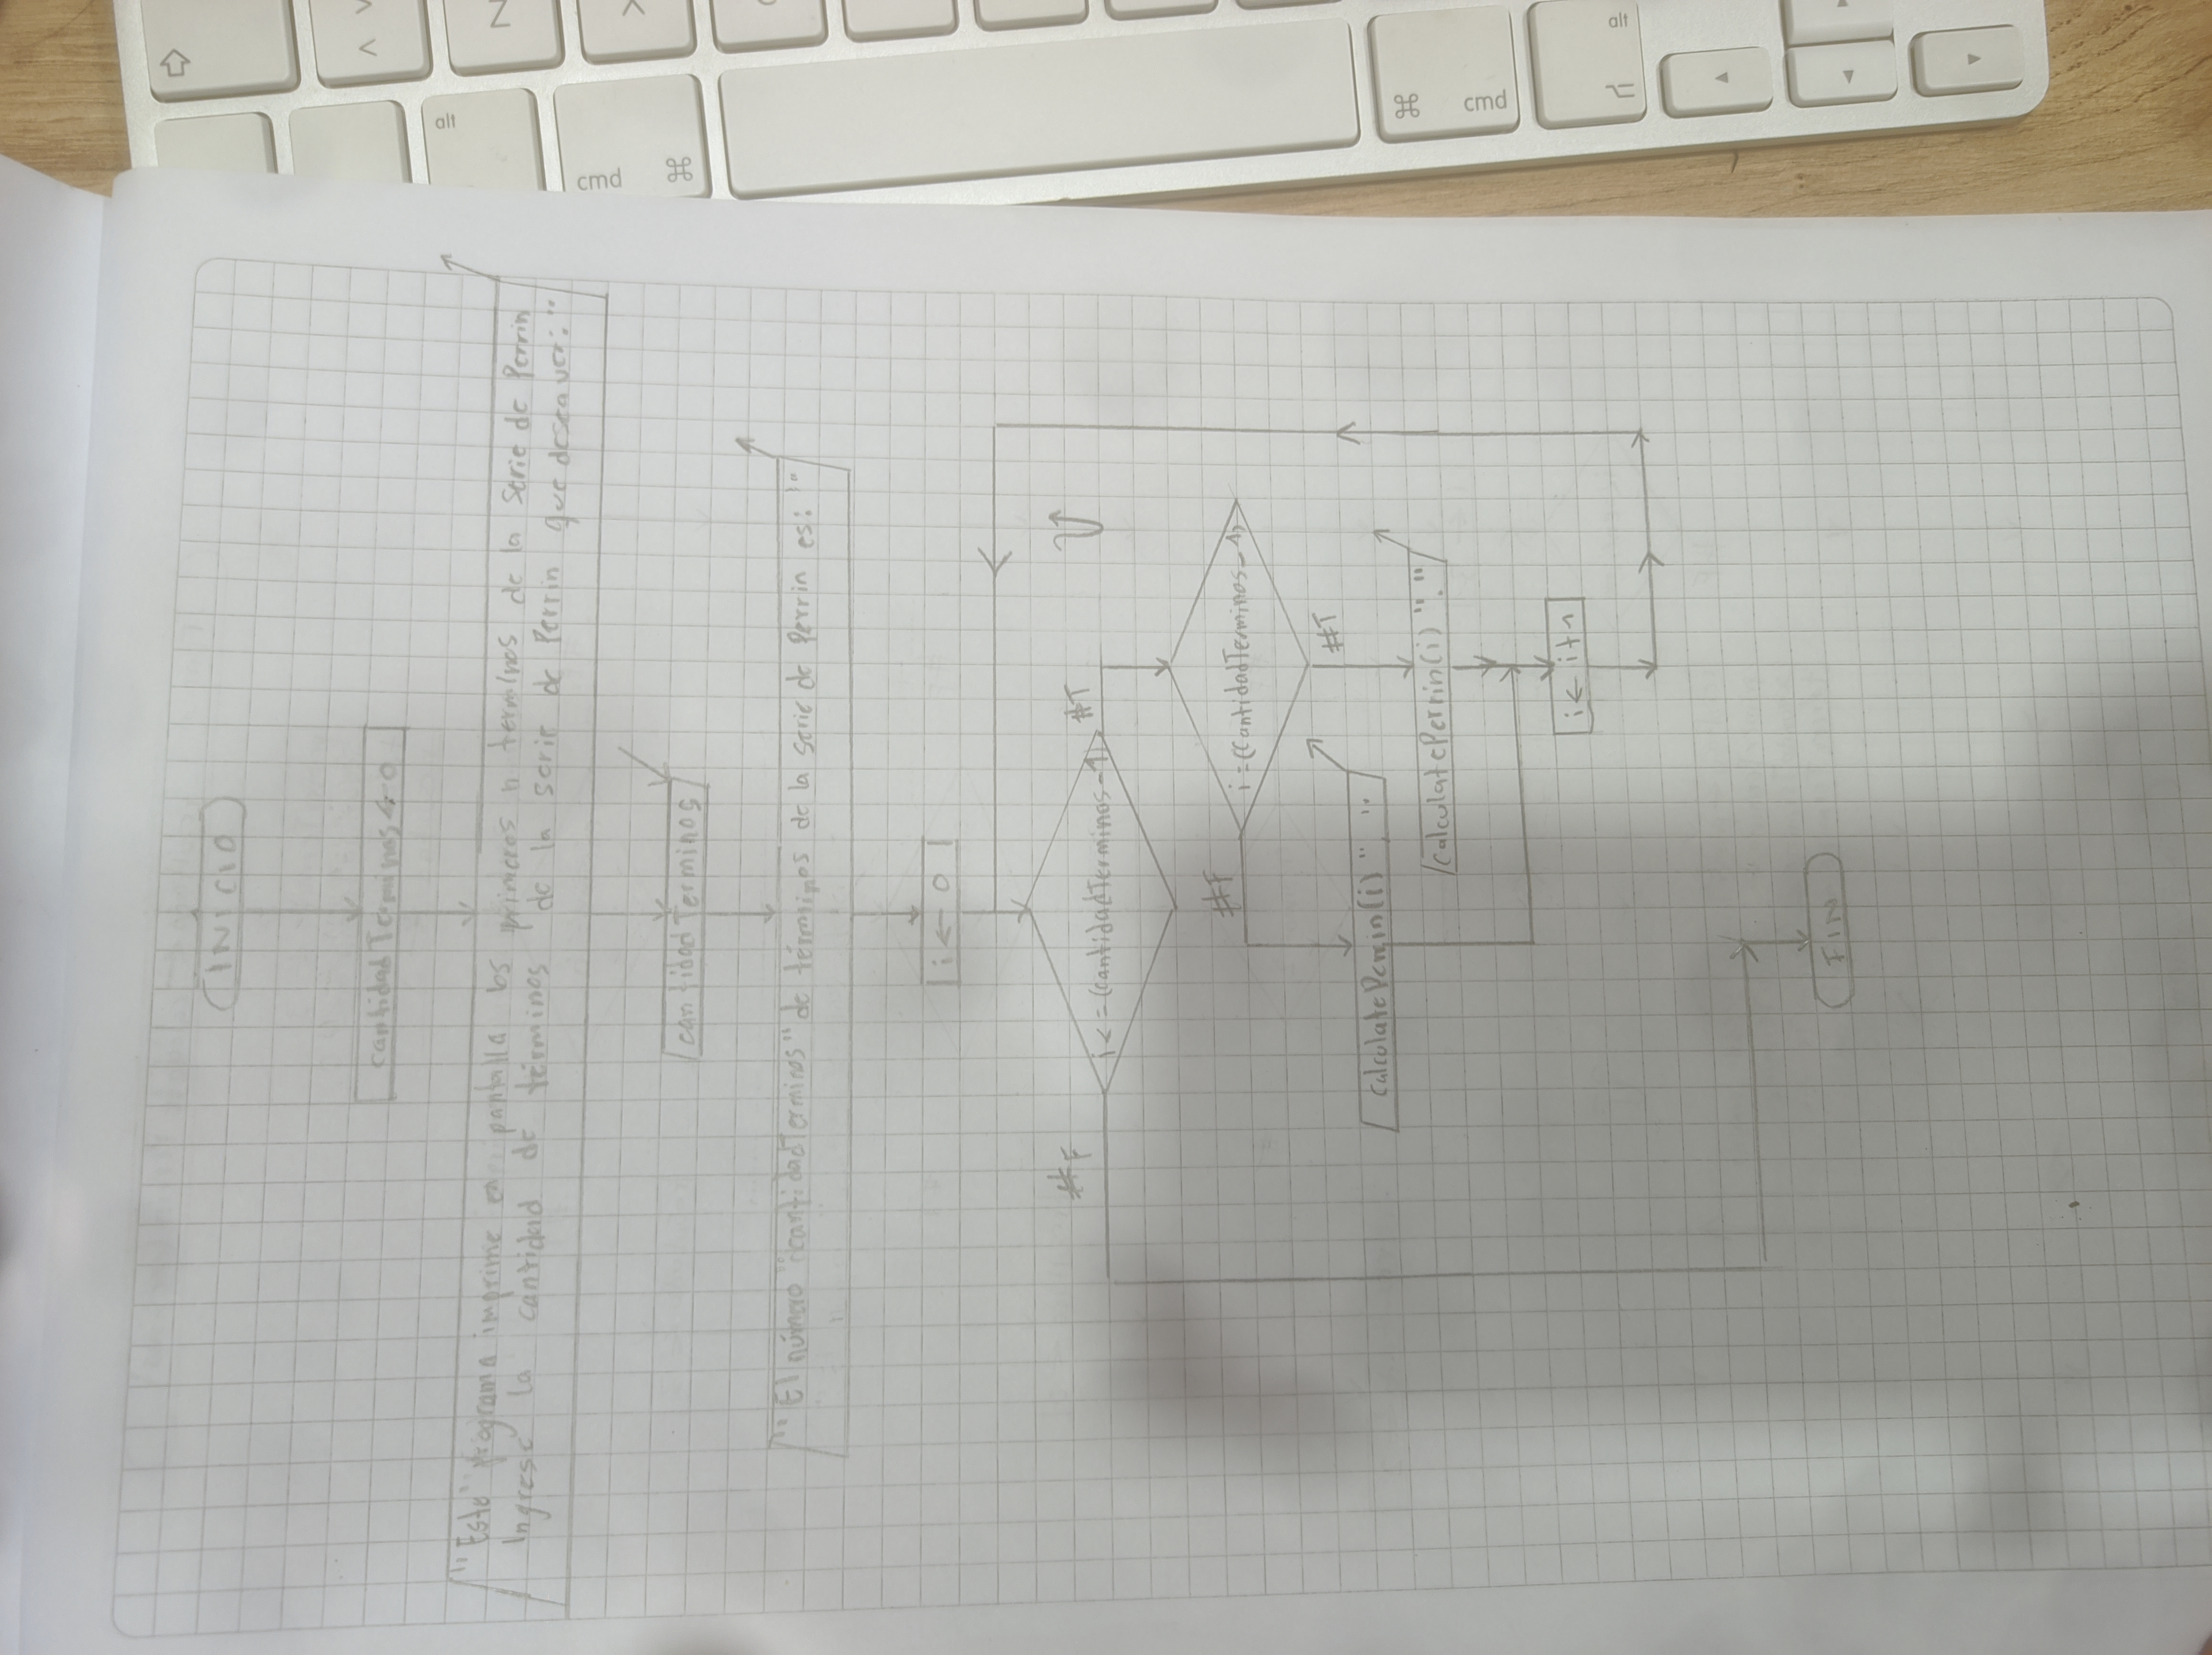
\includegraphics[width=14cm]{dfd/5.jpg}
  \caption{ DFD del punto 5}
  \label{fig: DFD del punto 5}
\end{figure}


\subsubsectionanum{Código}

\importsourcecode[]{c}{code/5.c}{}



\subsection{Punto 6}
	
	Ejemplo de pantalla:
 % Please add the following required packages to your document preamble:
% \usepackage{booktabs}
\begin{lstlisting}
Este programa imprime en pantalla los primeros n terminos de la serie de Padovan.
Ingrese la cantidad de términos de la serie de Padovan que desea ver: 6

La cantidad 6 de términos de la serie de Padovan son: 1, 0, 0, 1, 0, 1
\end{lstlisting}

\begin{lstlisting}
Este programa imprime en pantalla los primeros n terminos de la serie de Padovan.
Ingrese la cantidad de términos de la serie de Padovan que desea ver: 9

La cantidad 9 de términos de la serie de Padovan son: 1, 0, 0, 1, 0, 1, 1, 1, 2
\end{lstlisting}

\begin{lstlisting}
Este programa imprime en pantalla los primeros n terminos de la serie de Padovan.
Ingrese la cantidad de términos de la serie de Padovan que desea ver: 15

La cantidad 15 de términos de la serie de Padovan son: 1, 0, 0, 1, 0, 1, 1, 1, 2, 2, 3, 4, 5, 7, 9
\end{lstlisting}


\subsubsectionanum{DFD}
\begin{figure}
    \centering
    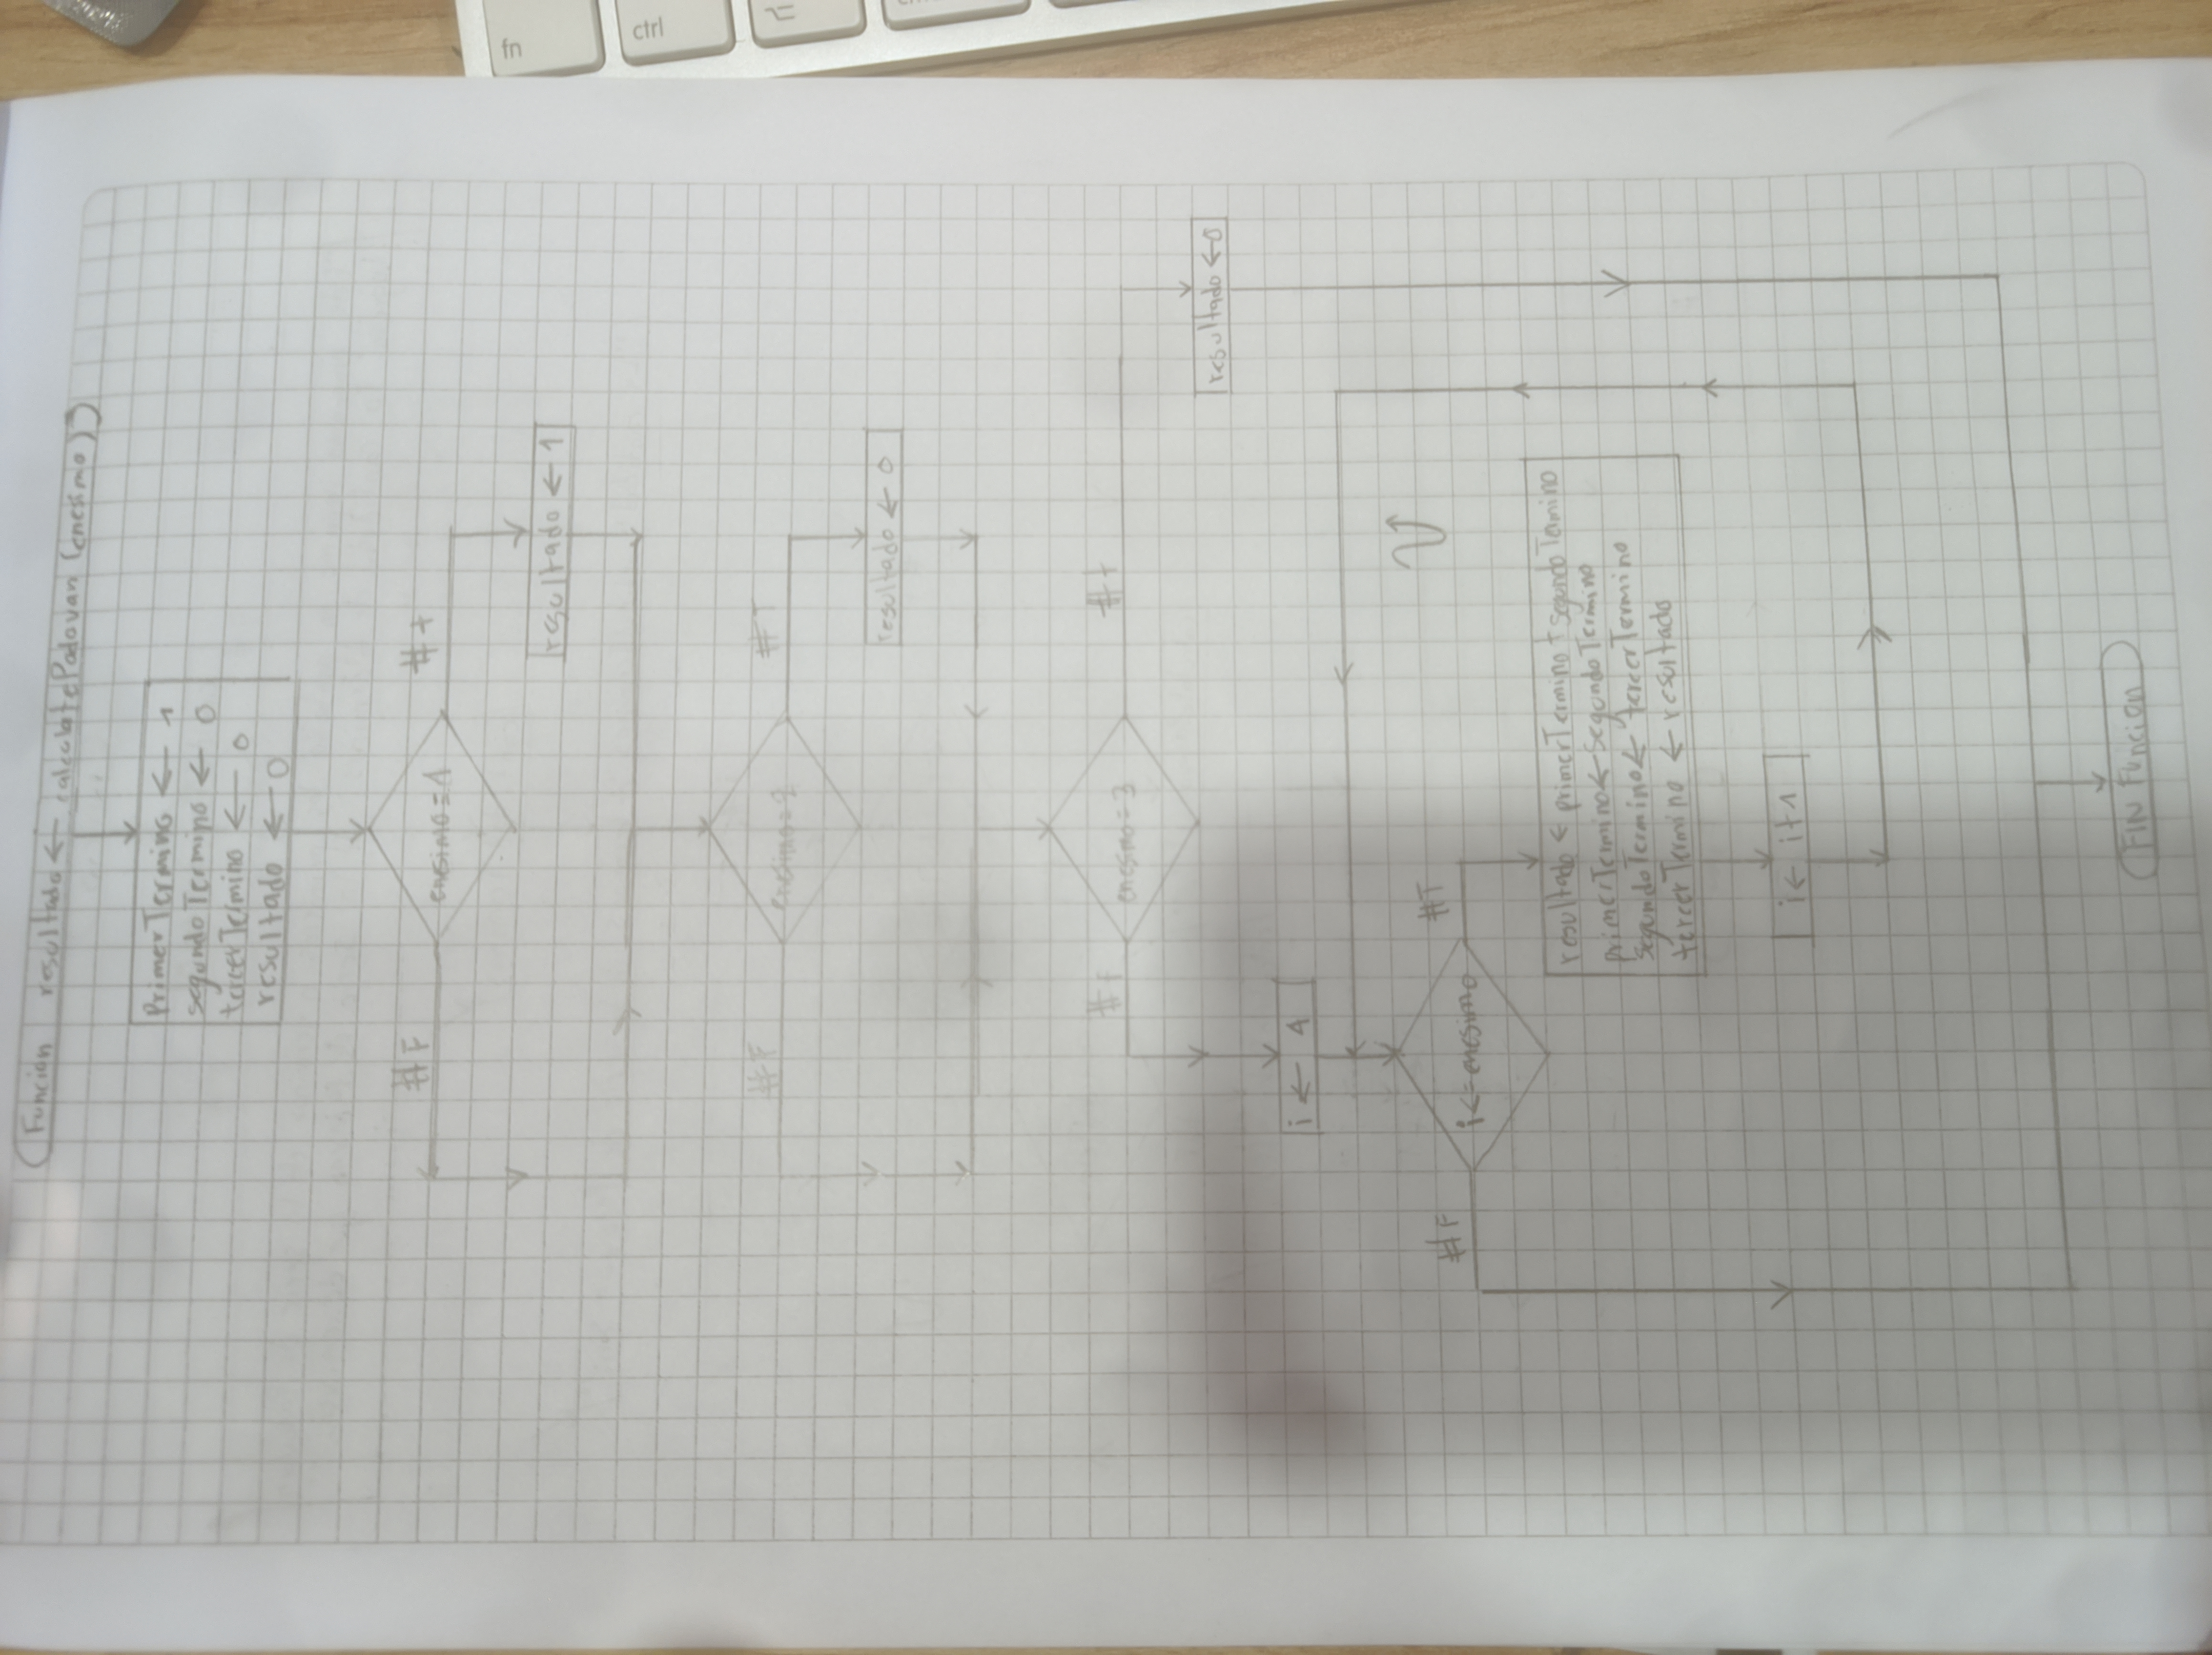
\includegraphics[width=14cm]{dfd/6.Funcion.jpg}
    \caption{ Función}
    \label{fig: Función}
\end{figure}  
\begin{figure}
  \centering
  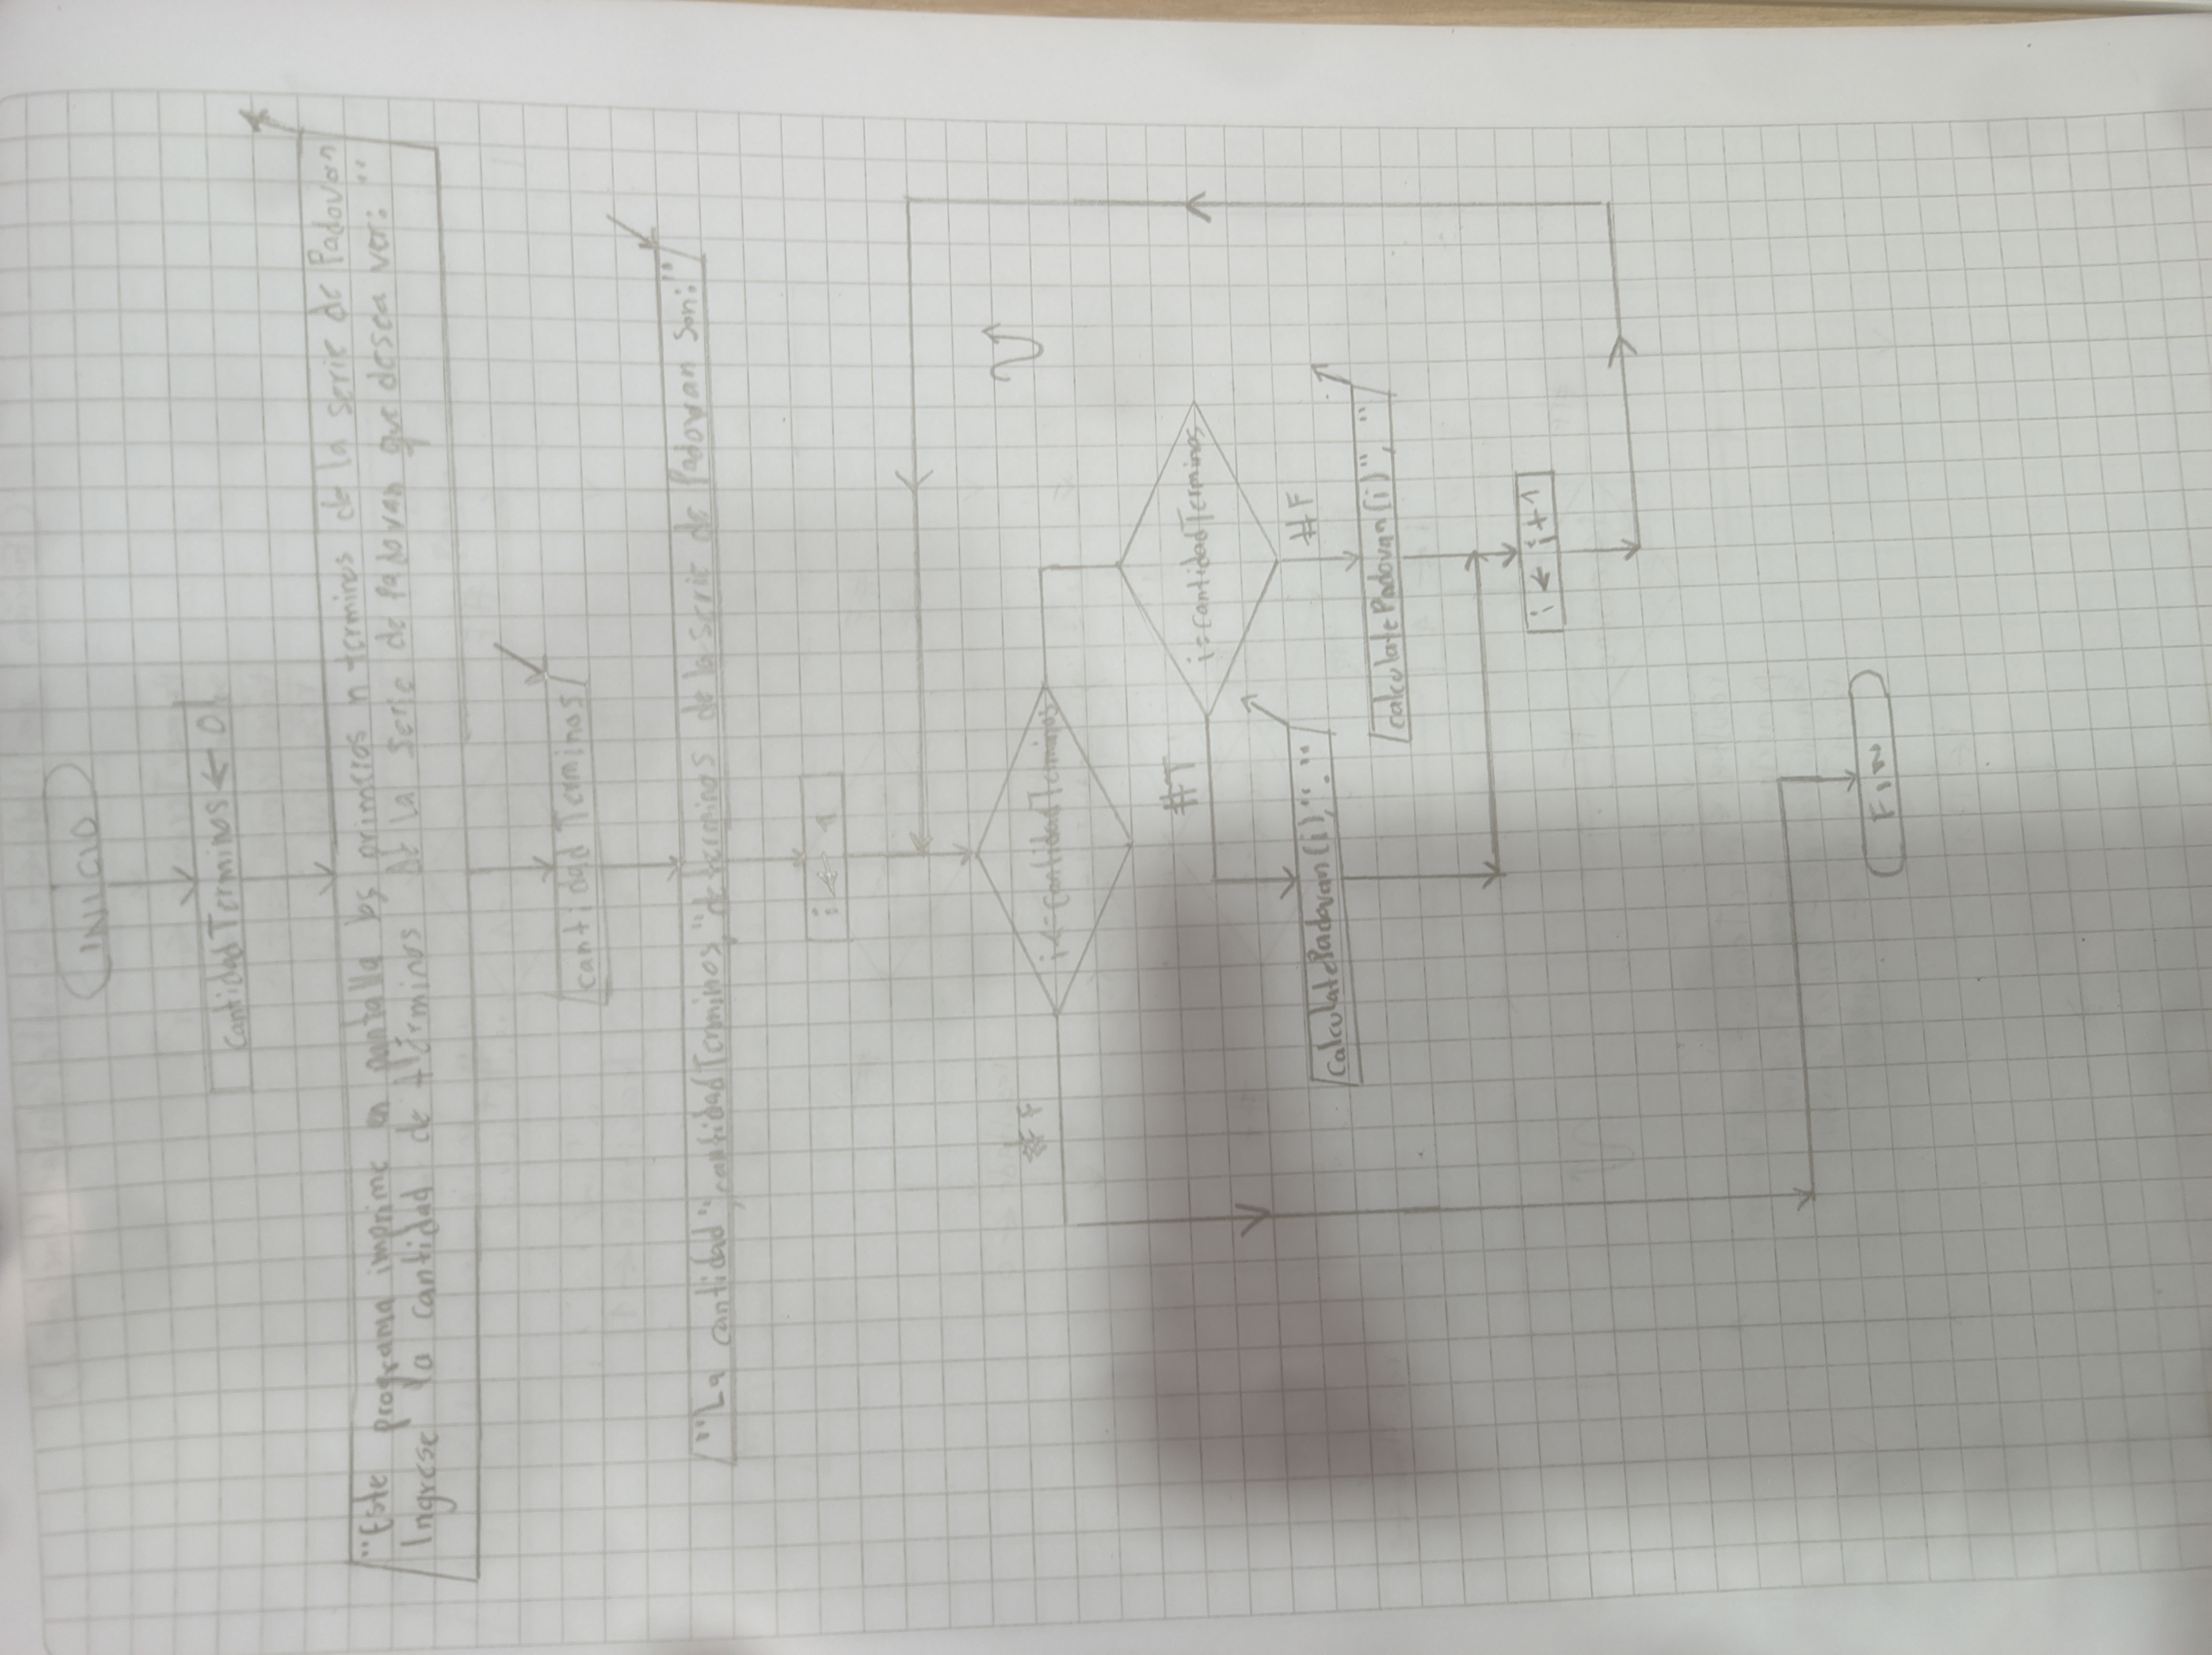
\includegraphics[width=14cm]{dfd/6.jpg}
  \caption{ DFD del punto 6}
  \label{fig: DFD del punto 6}
\end{figure}



\subsubsectionanum{Código}

\importsourcecode[]{c}{code/6.c}{}



\subsection{Punto 7}
	
	Ejemplo de pantalla:
 % Please add the following required packages to your document preamble:
% \usepackage{booktabs}
\begin{lstlisting}
Este programa imprime en pantalla los primeros n terminos de la secuencia de Narayana.
Esta serie comienza con los números 1, 1 y 1. Los siguientes términos
se calculan como la suma del término anterior y el número de parejas
de términos consecutivos anteriores que son diferentes.
Ingrese la cantidad de términos de la secuencia de Narayana que deseas que se impriman: 5


La cantidad 5 de términos de la serie de Narayana son: 1, 1, 1, 2, 3
\end{lstlisting}

\begin{lstlisting}
Este programa imprime en pantalla los primeros n terminos de la secuencia de Narayana.
Esta serie comienza con los números 1, 1 y 1. Los siguientes términos
se calculan como la suma del término anterior y el número de parejas
de términos consecutivos anteriores que son diferentes.
Ingrese la cantidad de términos de la secuencia de Narayana que deseas que se impriman: 9


La cantidad 9 de términos de la serie de Narayana son: 1, 1, 1, 2, 3, 4, 6, 9, 13
\end{lstlisting}

\begin{lstlisting}
Este programa imprime en pantalla los primeros n terminos de la secuencia de Narayana.
Esta serie comienza con los números 1, 1 y 1. Los siguientes términos
se calculan como la suma del término anterior y el número de parejas
de términos consecutivos anteriores que son diferentes.
Ingrese la cantidad de términos de la secuencia de Narayana que deseas que se impriman: 15


La cantidad 15 de términos de la serie de Narayana son: 1, 1, 1, 2, 3, 4, 6, 9, 13, 19, 28, 41, 60, 88, 129
\end{lstlisting}

\subsubsectionanum{DFD}
\subsubsectionanum{DFD}
\begin{figure}
    \centering
    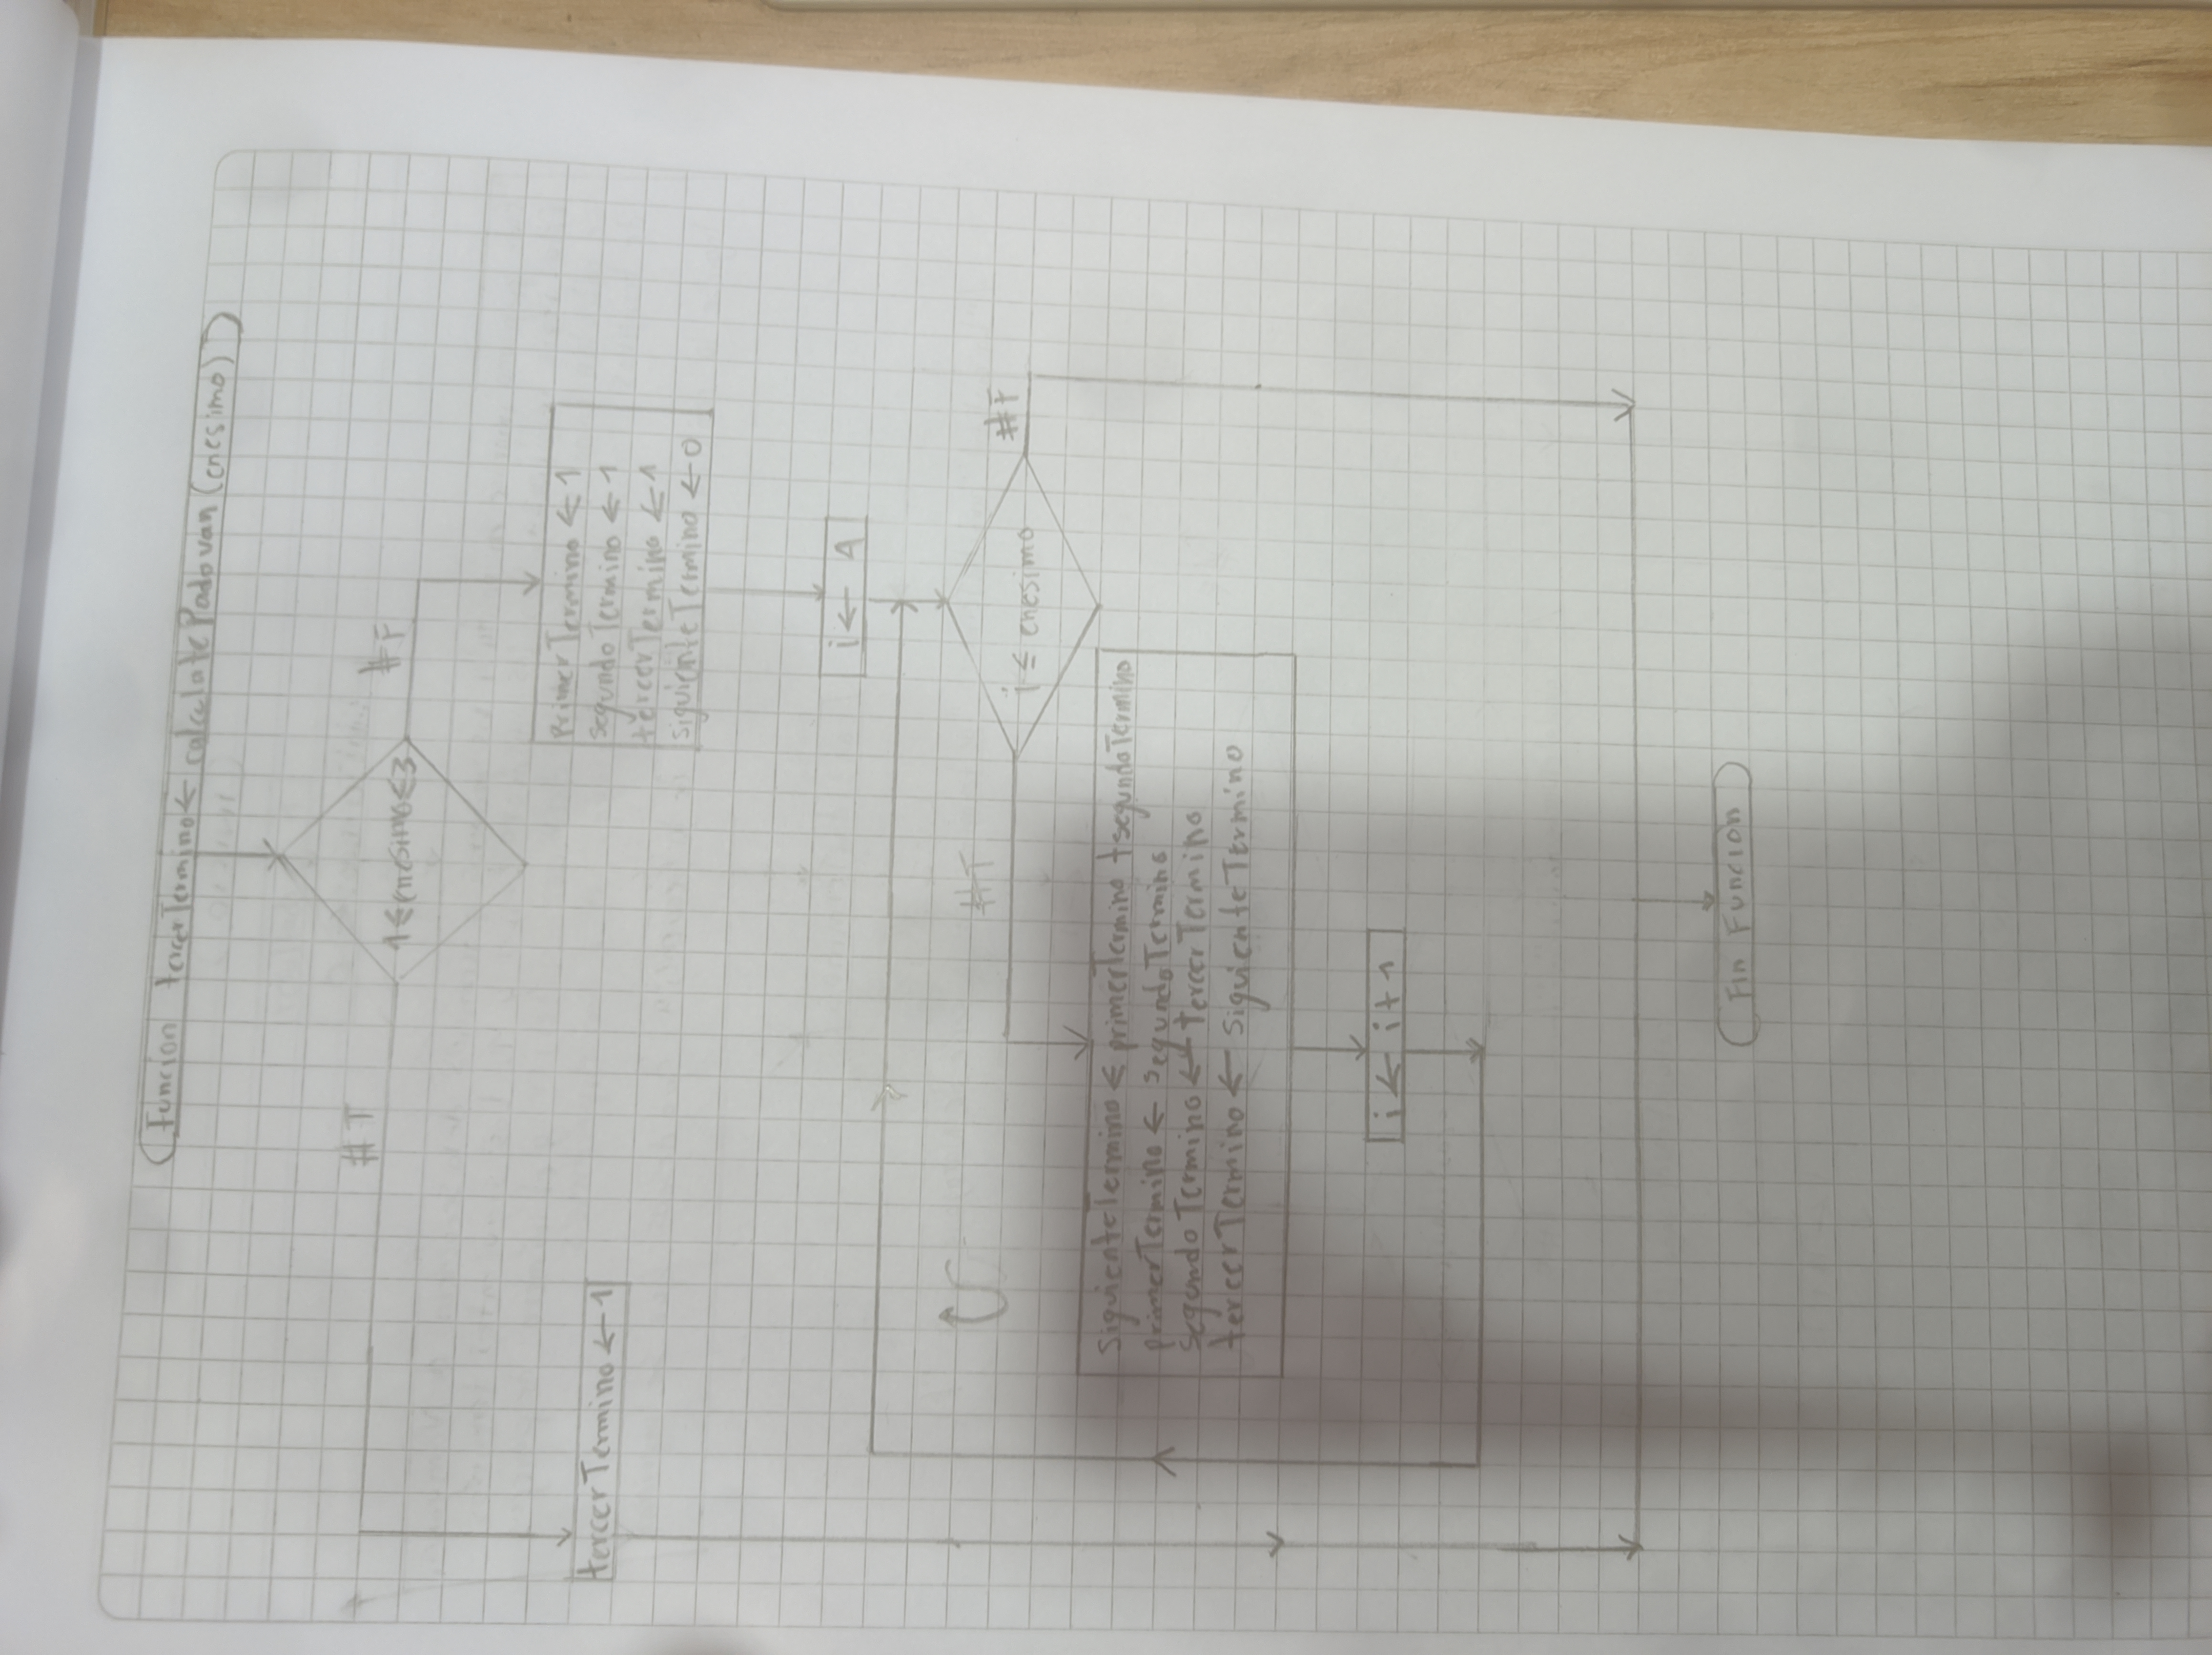
\includegraphics[width=14cm]{dfd/7.Funcion.jpg}
    \caption{ Función}
    \label{fig: Función}
\end{figure}  
\begin{figure}
  \centering
  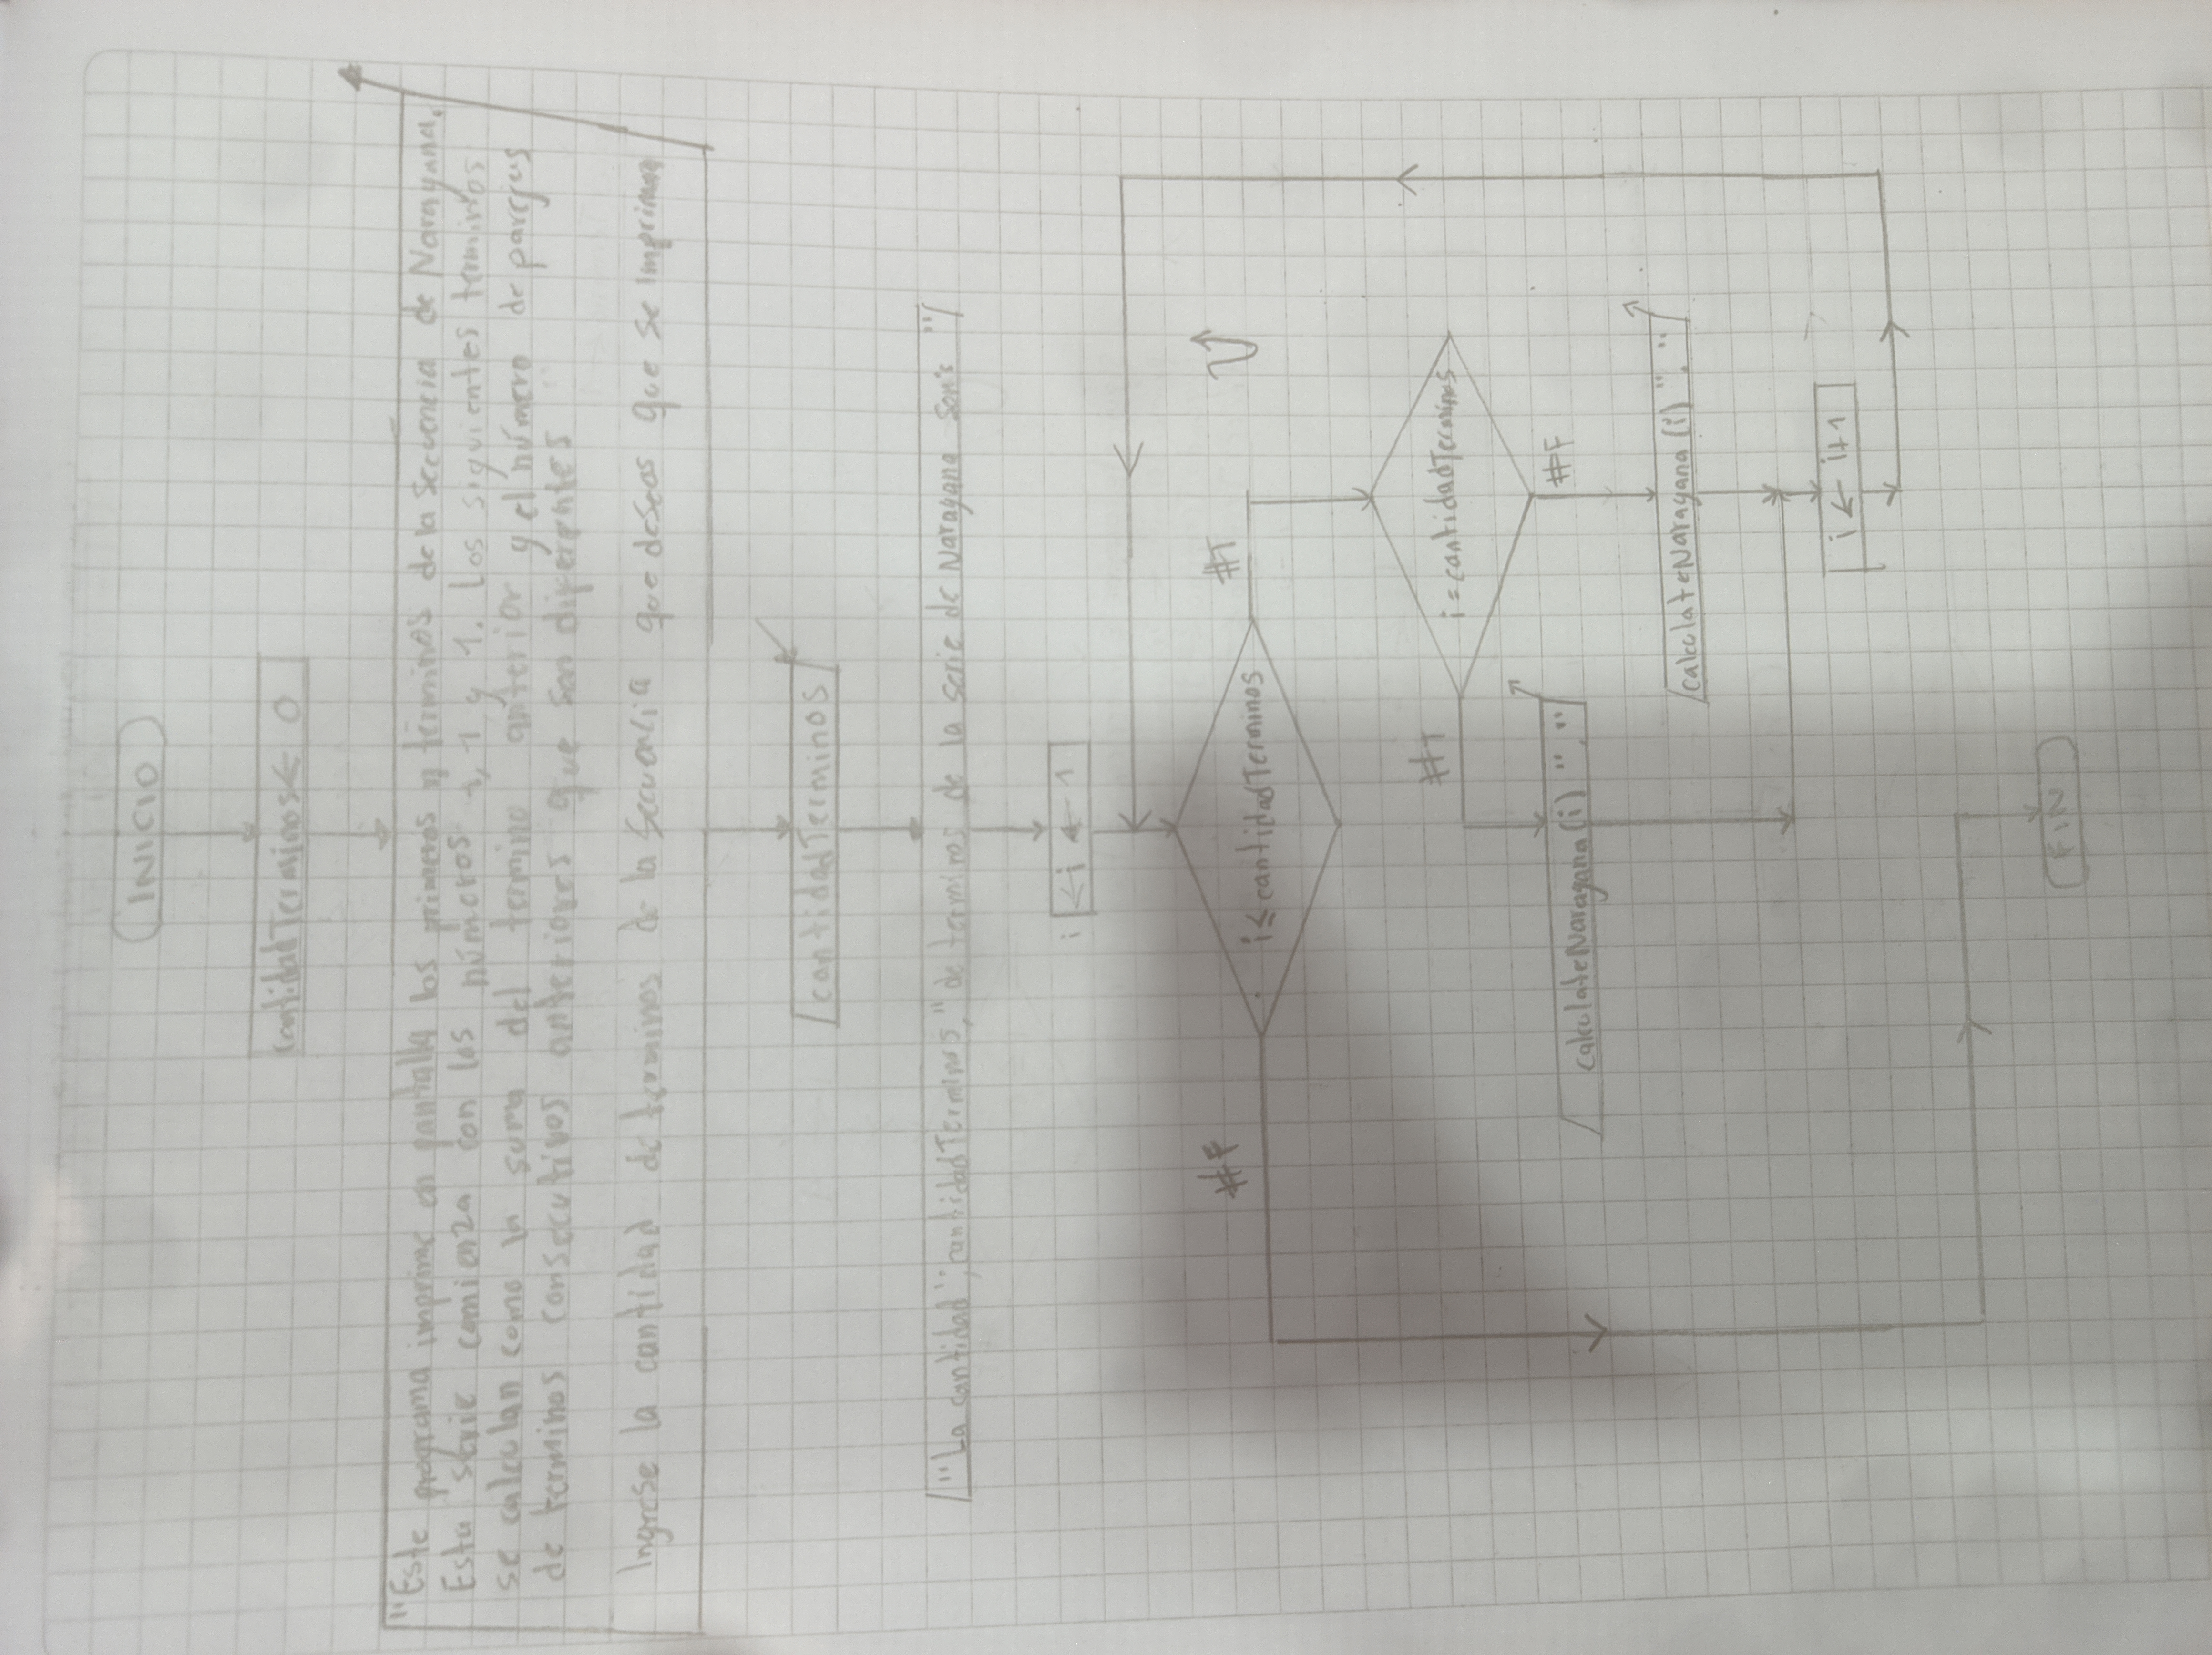
\includegraphics[width=14cm]{dfd/7.jpg}
  \caption{ DFD del punto 7}
  \label{fig: DFD del punto 7}
\end{figure}


\subsubsectionanum{Código}

\importsourcecode[]{c}{code/7.c}{}




\subsection{Punto 8}
	
	Ejemplo de pantalla:
 % Please add the following required packages to your document preamble:
% \usepackage{booktabs}
\begin{lstlisting}
Este programa imprime en pantalla hasta el termino enesimo que solicites.
De la serie Catalan es una secuencia de números que aparece en diversos problemas de conteo en matemáticas
Comienza con los números 1, 1 y los siguientes términos se calculan como la suma de los productos de los términos anteriores.
Ingrese la cantidad de términos de la serie de Padovan que desea ver: 5

La cantidad 5 de términos de la serie de Catalan es: 1, 1, 2, 5, 14.
\end{lstlisting}

\begin{lstlisting}
Este programa imprime en pantalla hasta el termino enesimo que solicites.
De la serie Catalan es una secuencia de números que aparece en diversos problemas de conteo en matemáticas
Comienza con los números 1, 1 y los siguientes términos se calculan como la suma de los productos de los términos anteriores.
Ingrese la cantidad de términos de la serie de Padovan que desea ver: 9

La cantidad 9 de términos de la serie de Catalan es: 1, 1, 2, 5, 14, 42, 132, 429, 1430.
\end{lstlisting}

\begin{lstlisting}
Este programa imprime en pantalla hasta el termino enesimo que solicites.
De la serie Catalan es una secuencia de números que aparece en diversos problemas de conteo en matemáticas
Comienza con los números 1, 1 y los siguientes términos se calculan como la suma de los productos de los términos anteriores.
Ingrese la cantidad de términos de la serie de Padovan que desea ver: 15

La cantidad 15 de términos de la serie de Catalan es: 1, 1, 2, 5, 14, 42, 132, 429, 1430, 4862, 16796, 58786, 208012, 742900, 2674440
\end{lstlisting}


\subsubsectionanum{DFD}
\begin{figure}
  \centering
  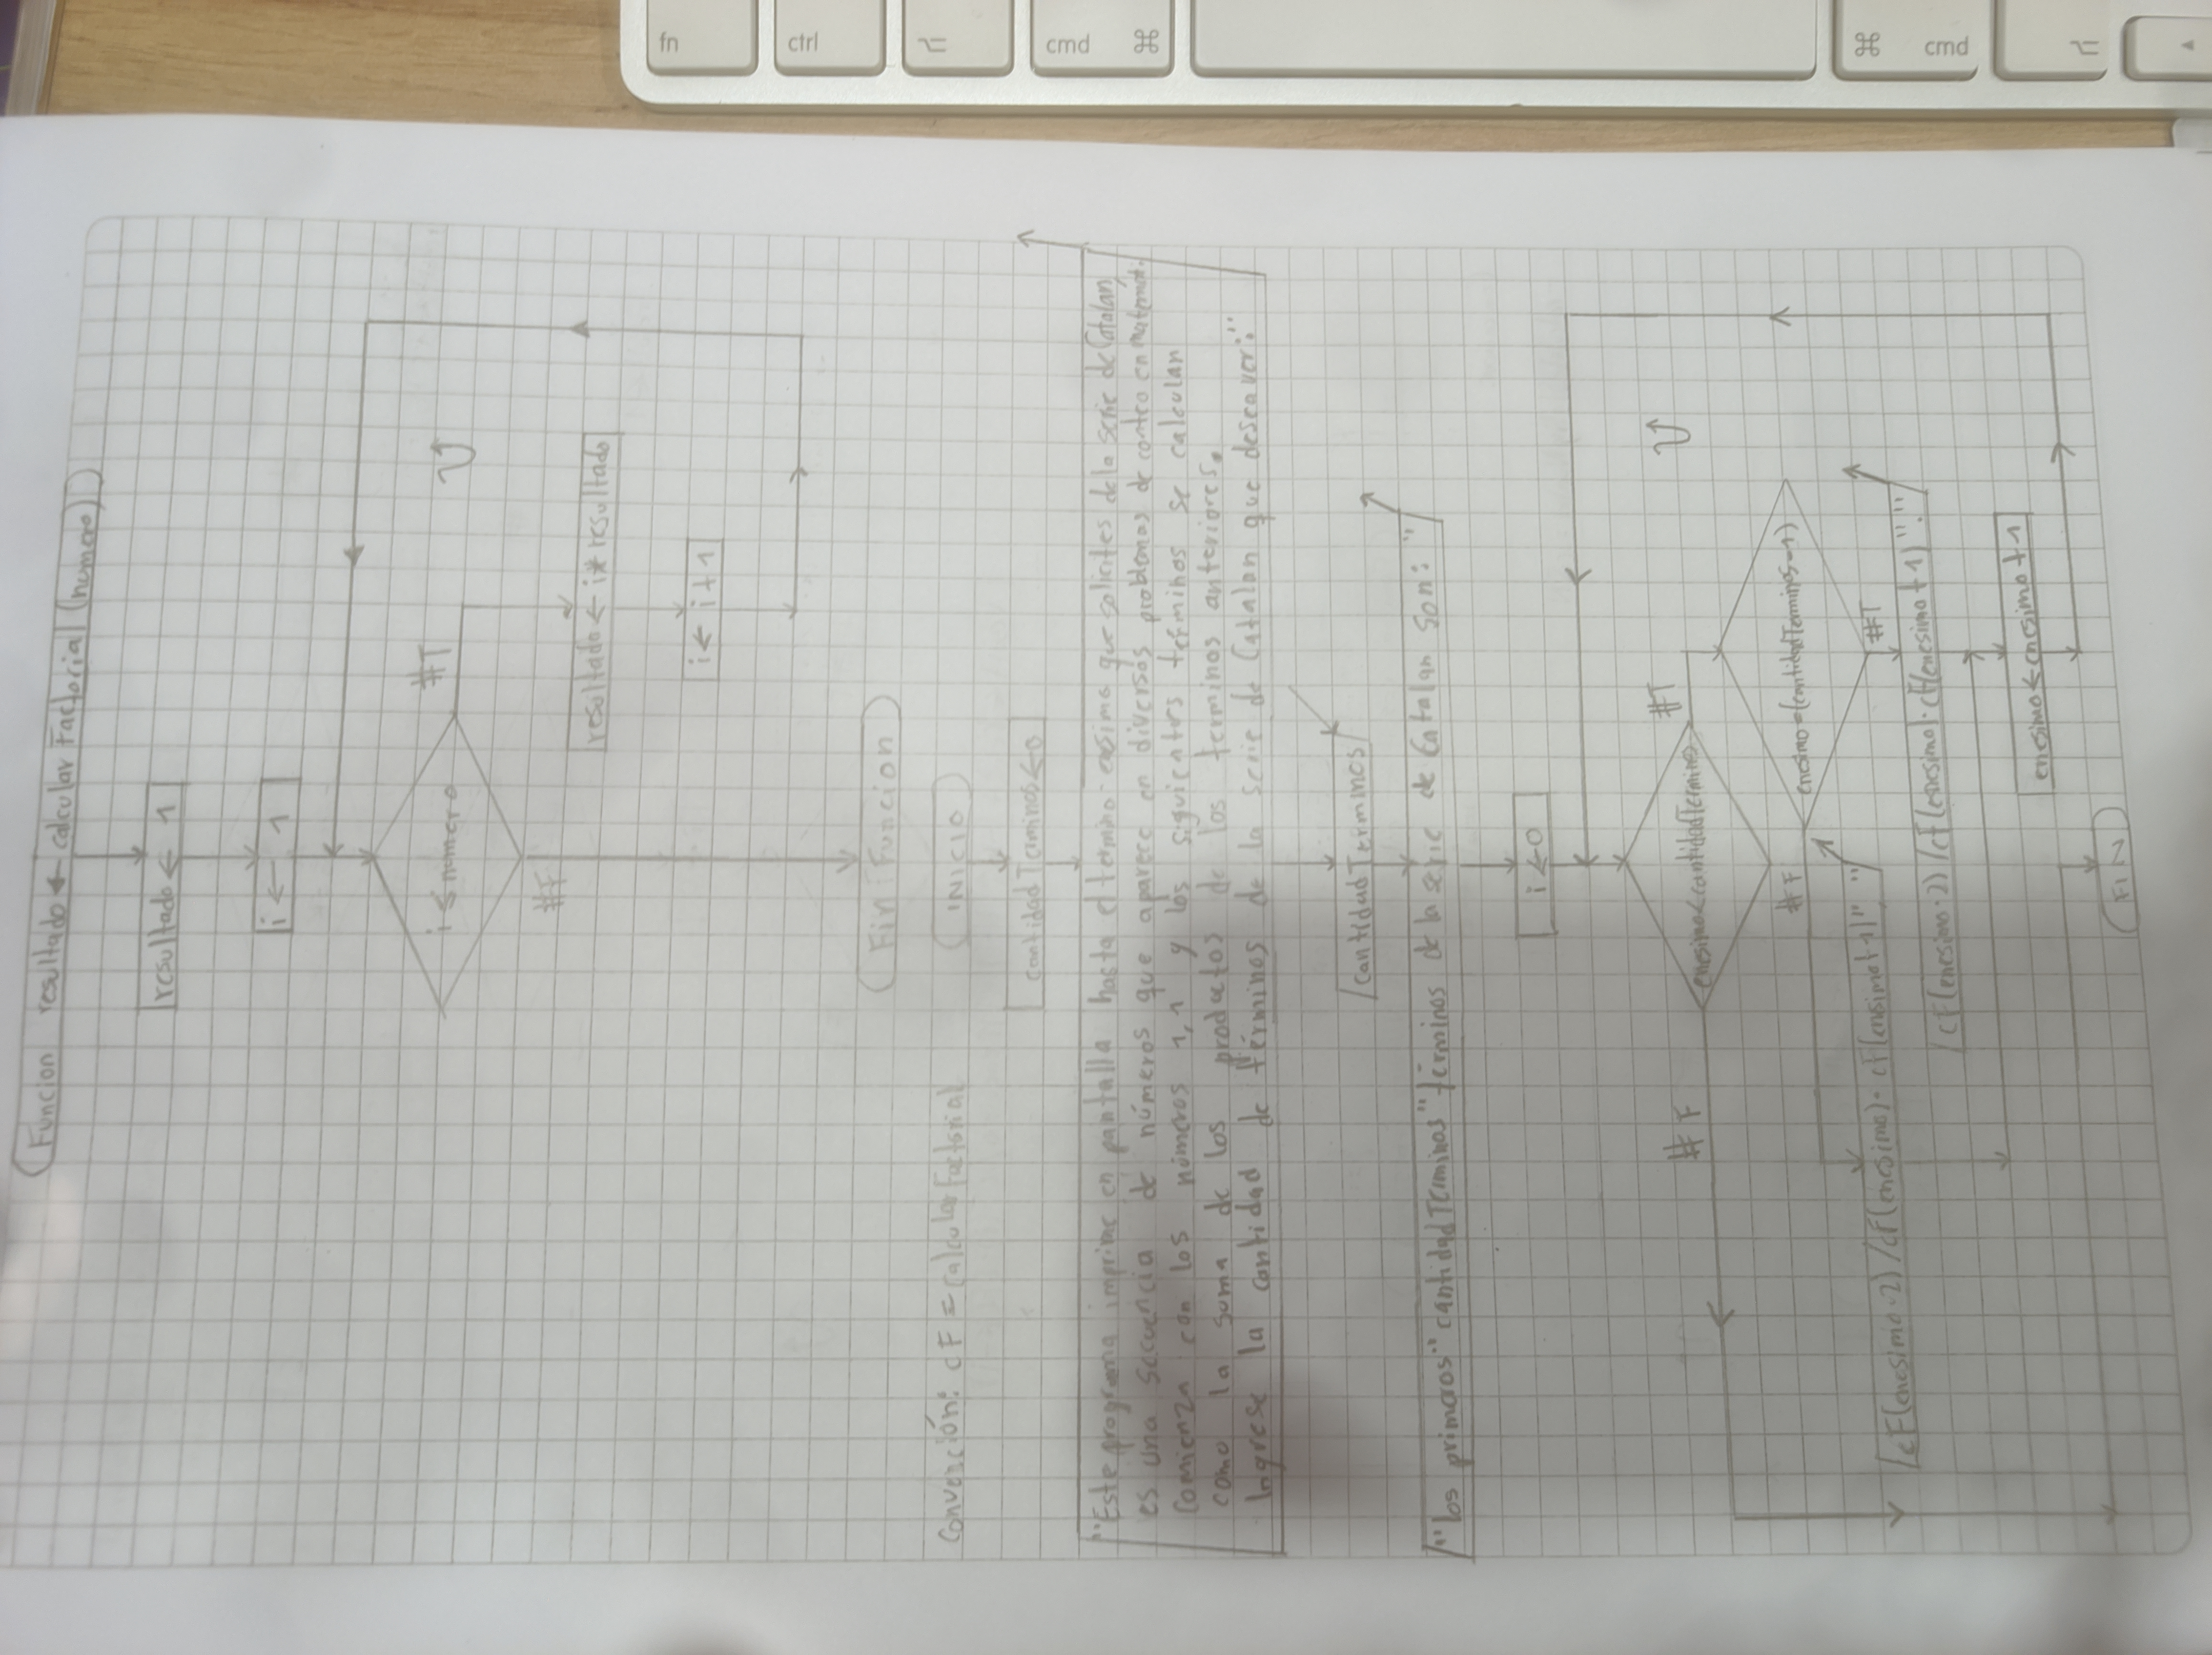
\includegraphics[width=14cm]{dfd/8.jpg}
  \caption{ DFD del punto 8}
  \label{fig: DFD del punto 8}
\end{figure}



\subsubsectionanum{Código}

\importsourcecode[]{c}{code/8.c}{}



\subsection{Punto 9}
	
	Ejemplo de pantalla:
 % Please add the following required packages to your document preamble:
% \usepackage{booktabs}
\begin{lstlisting}
Este programa va imprimir los términos que le solicites de la serie de Bell: 
Esta serie cuenta el número de particiones no vacías de un conjunto de n elementos. 
Comienza con los números 1, 1 y los siguientes términos se calculan como la suma de 
los términos anteriores multiplicados por los números naturales consecutivos.
Ingrese a continuación el número de términos deseados: 5

Los primeros 5 términos de la serie de Bell son: 1, 1, 2, 5, 15
\end{lstlisting}

\begin{lstlisting}
Este programa va imprimir los términos que le solicites de la serie de Bell: 
Esta serie cuenta el número de particiones no vacías de un conjunto de n elementos. 
Comienza con los números 1, 1 y los siguientes términos se calculan como la suma de 
los términos anteriores multiplicados por los números naturales consecutivos.
Ingrese a continuación el número de términos deseados: 9

Los primeros 9 términos de la serie de Bell son: 1, 1, 2, 5, 15, 52, 203, 877, 4140
\end{lstlisting}

\begin{lstlisting}
Este programa va imprimir los términos que le solicites de la serie de Bell: 
Esta serie cuenta el número de particiones no vacías de un conjunto de n elementos. 
Comienza con los números 1, 1 y los siguientes términos se calculan como la suma de 
los términos anteriores multiplicados por los números naturales consecutivos.
Ingrese a continuación el número de términos deseados: 15

Los primeros 15 términos de la serie de Bell son: 1, 1, 2, 5, 15, 52, 203, 877, 4140, 21147, 115975, 678570, 4213597, 27644437, 77914768.
\end{lstlisting}

\subsubsectionanum{DFD}
\begin{figure}
    \centering
    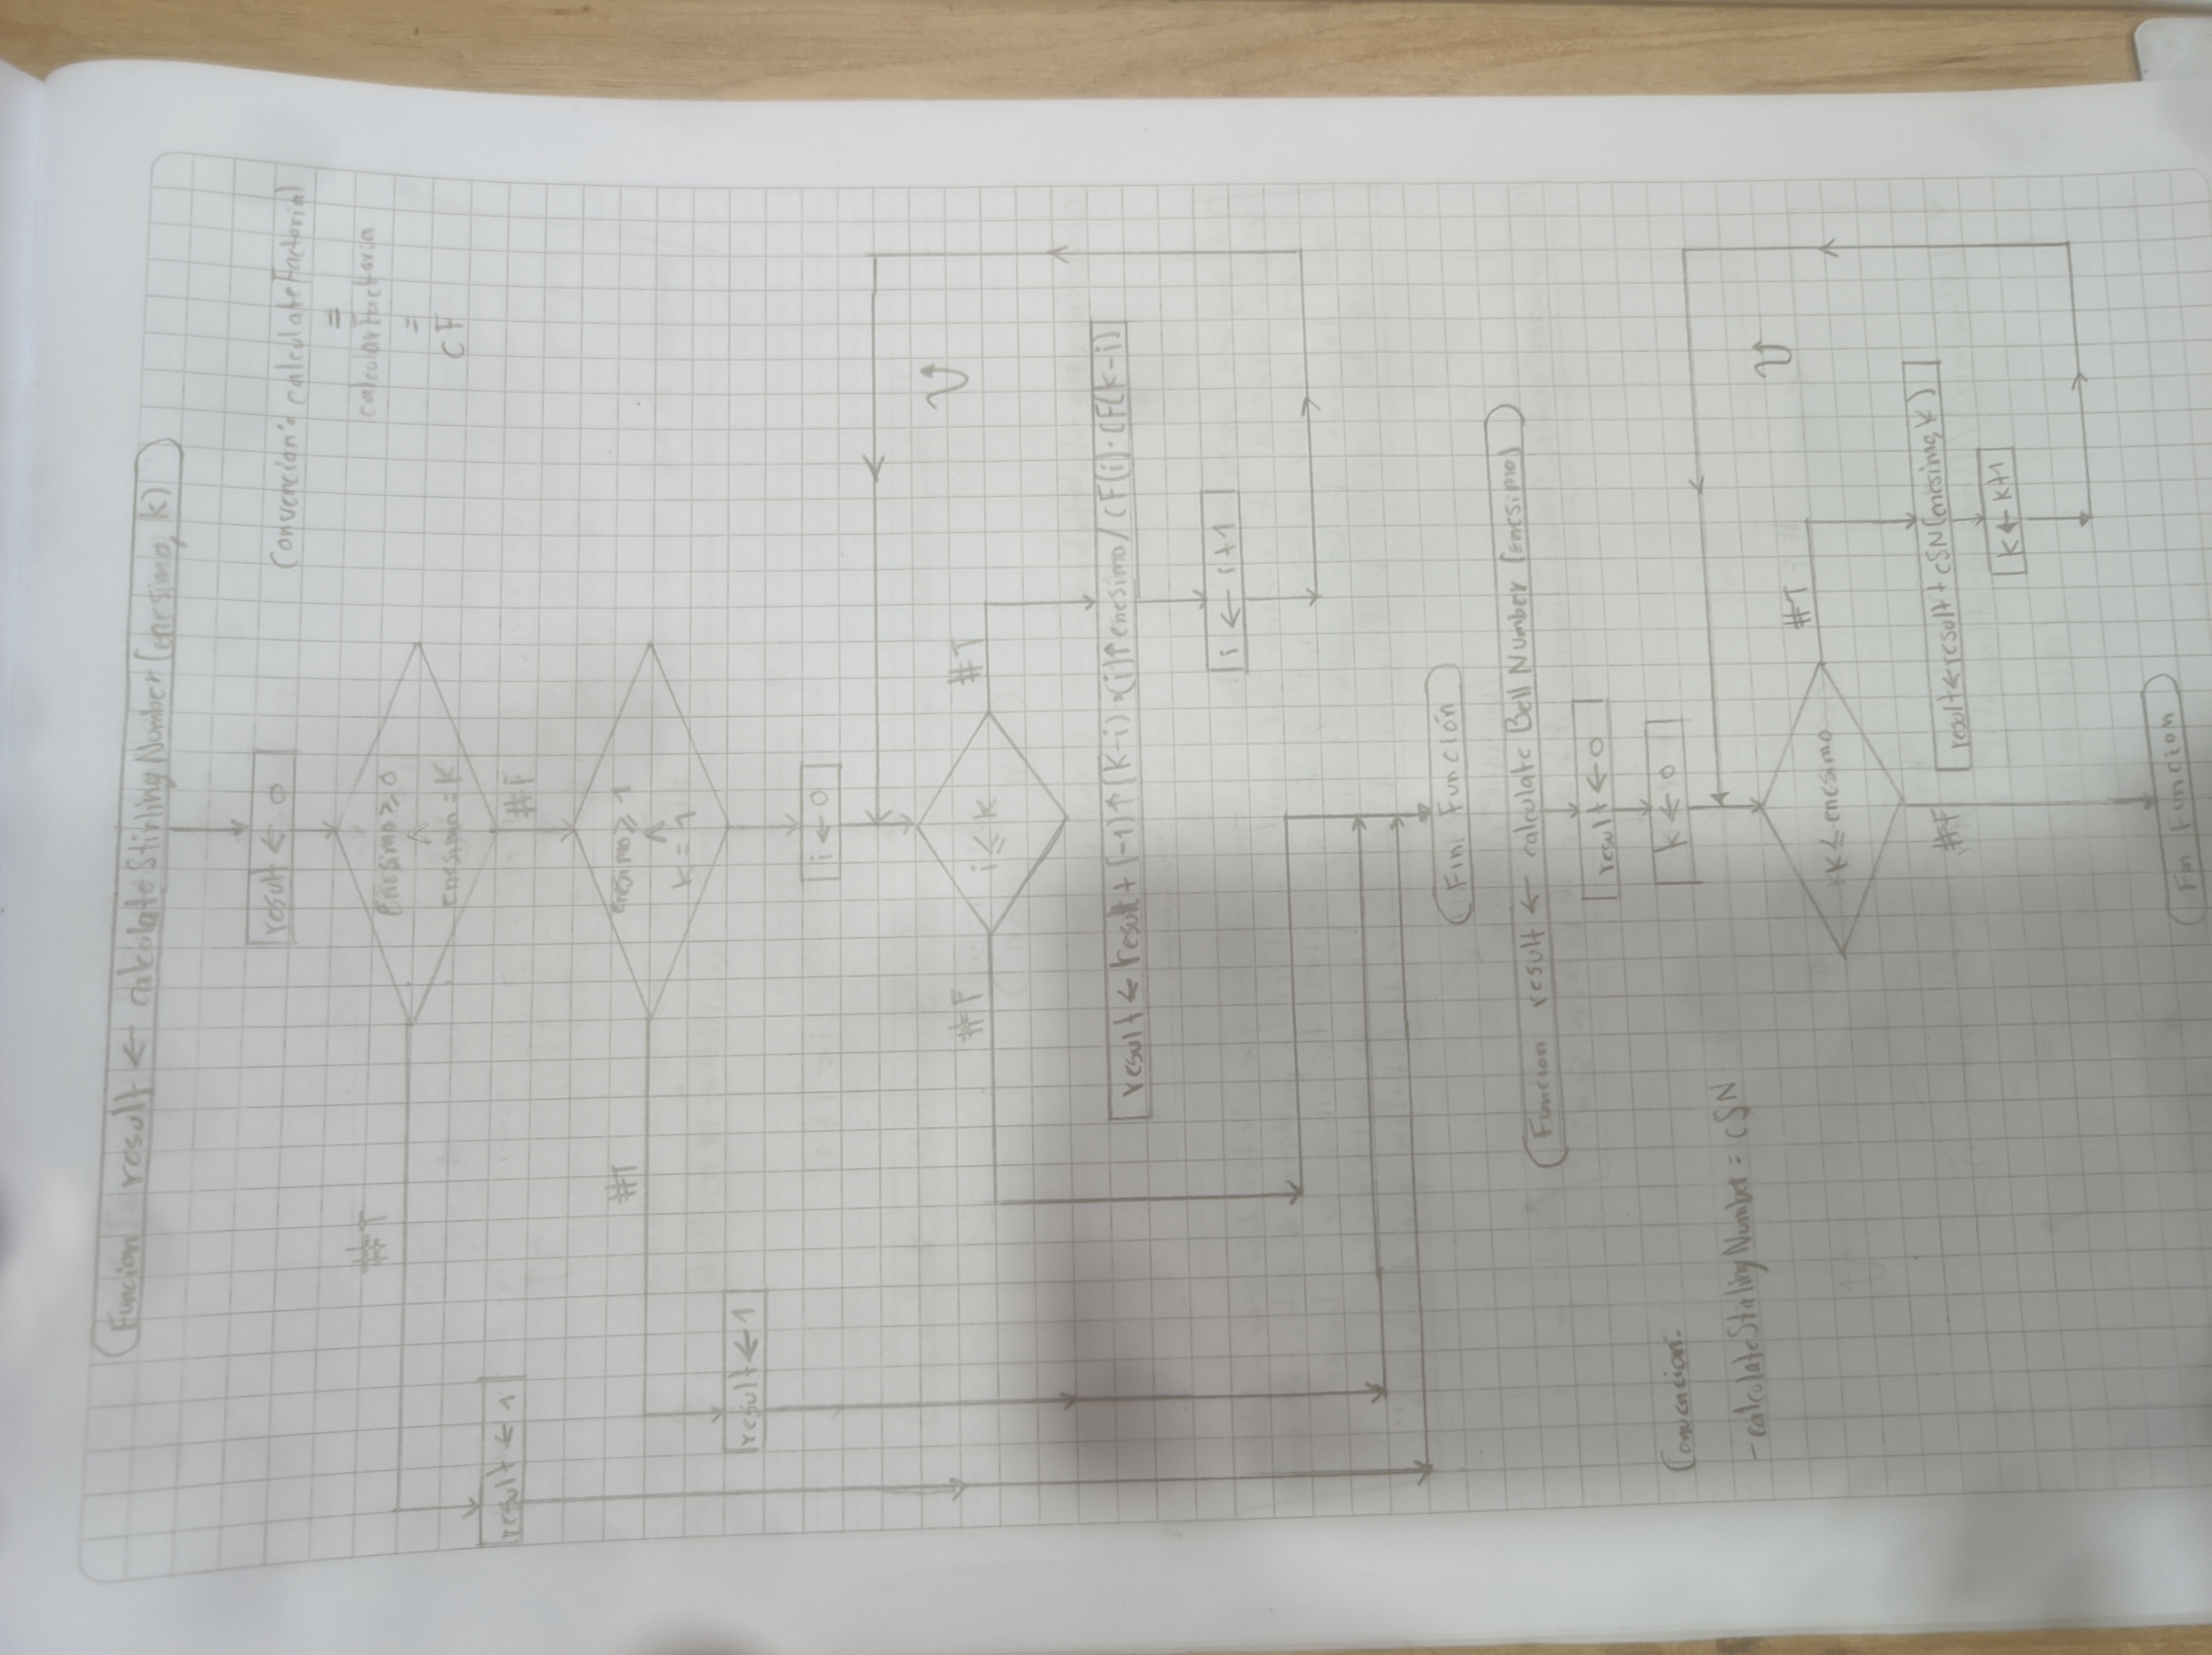
\includegraphics[width=14cm]{dfd/9.Funcion.jpg}
    \caption{ Función}
    \label{fig: Función}
\end{figure}  
\begin{figure}
  \centering
  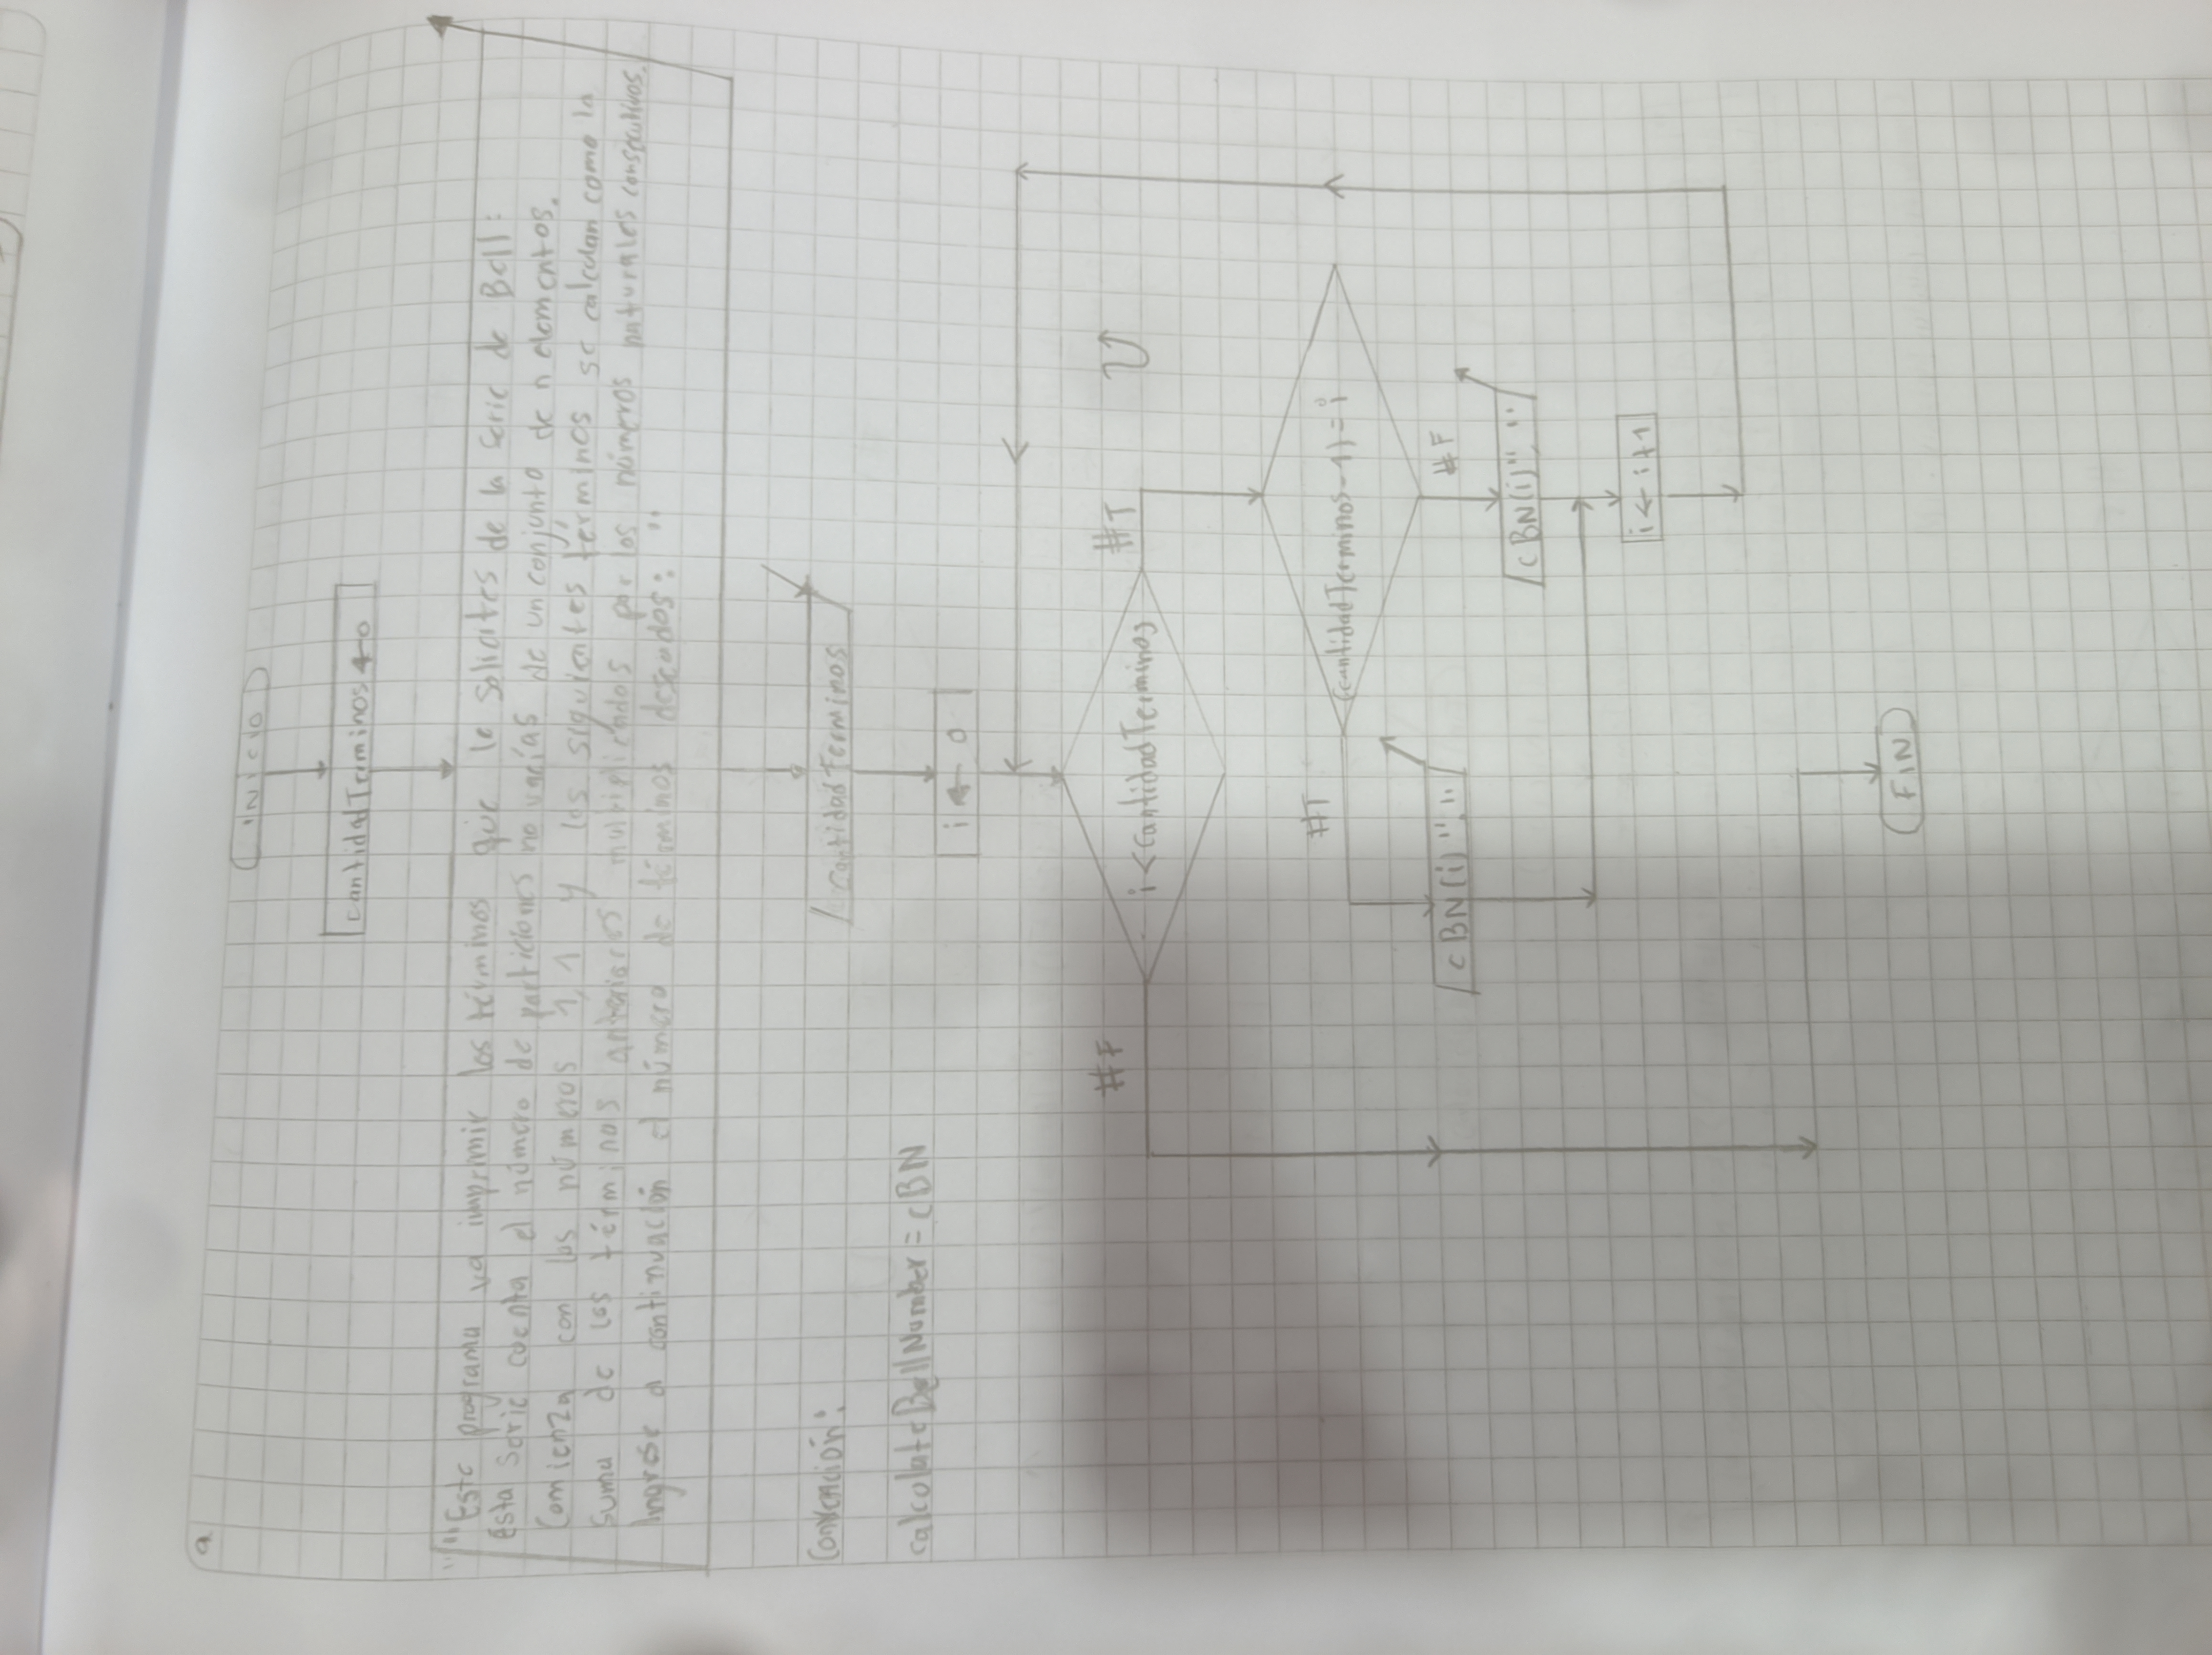
\includegraphics[width=14cm]{dfd/9.jpg}
  \caption{ DFD del punto 9}
  \label{fig: DFD del punto 9}
\end{figure}

\subsubsectionanum{Código}

\importsourcecode[]{c}{code/9.c}{}


\subsection{Punto 10}
	
	Ejemplo de pantalla:
 % Please add the following required packages to your document preamble:
% \usepackage{booktabs}
\begin{lstlisting}
Este programa presenta la Serie de Motzkin: Esta serie cuenta el número de caminos no cruzados de 
longitud n en una retícula tridimensional. Comienza con los números 1, 1 y los siguientes términos 
se calculan como la suma de los términos anteriores y, la suma de los términos anteriores 
menos el tercer término anterior. 
La fórmula para el enésimo número de Motzkin es M(n) = M(n-1) + Σ(k=0, n-2) M(k)M(n-2-k), donde M(0) = 1 y M(1) = 1.
Ingrese el número de términos que desea: 6
1, 1, 2, 4, 9, 21.
\end{lstlisting}

\begin{lstlisting}
Este programa presenta la Serie de Motzkin: Esta serie cuenta el número de caminos no cruzados de 
longitud n en una retícula tridimensional. Comienza con los números 1, 1 y los siguientes términos 
se calculan como la suma de los términos anteriores y, la suma de los términos anteriores 
menos el tercer término anterior. 
La fórmula para el enésimo número de Motzkin es M(n) = M(n-1) + Σ(k=0, n-2) M(k)M(n-2-k), donde M(0) = 1 y M(1) = 1.
Ingrese el número de términos que desea: 9
1, 1, 2, 4, 9, 21, 51, 127, 323.
\end{lstlisting}

\begin{lstlisting}
Este programa presenta la Serie de Motzkin: Esta serie cuenta el número de caminos no cruzados de 
longitud n en una retícula tridimensional. Comienza con los números 1, 1 y los siguientes términos 
se calculan como la suma de los términos anteriores y, la suma de los términos anteriores 
menos el tercer término anterior. 
La fórmula para el enésimo número de Motzkin es M(n) = M(n-1) + Σ(k=0, n-2) M(k)M(n-2-k), donde M(0) = 1 y M(1) = 1.
Ingrese el número de términos que desea: 15
1, 1, 2, 4, 9, 21, 51, 127, 323, 835, 2188, 5798, 15511, 41835, 113634.
\end{lstlisting}

\subsubsectionanum{DFD}
\begin{figure}
    \centering
    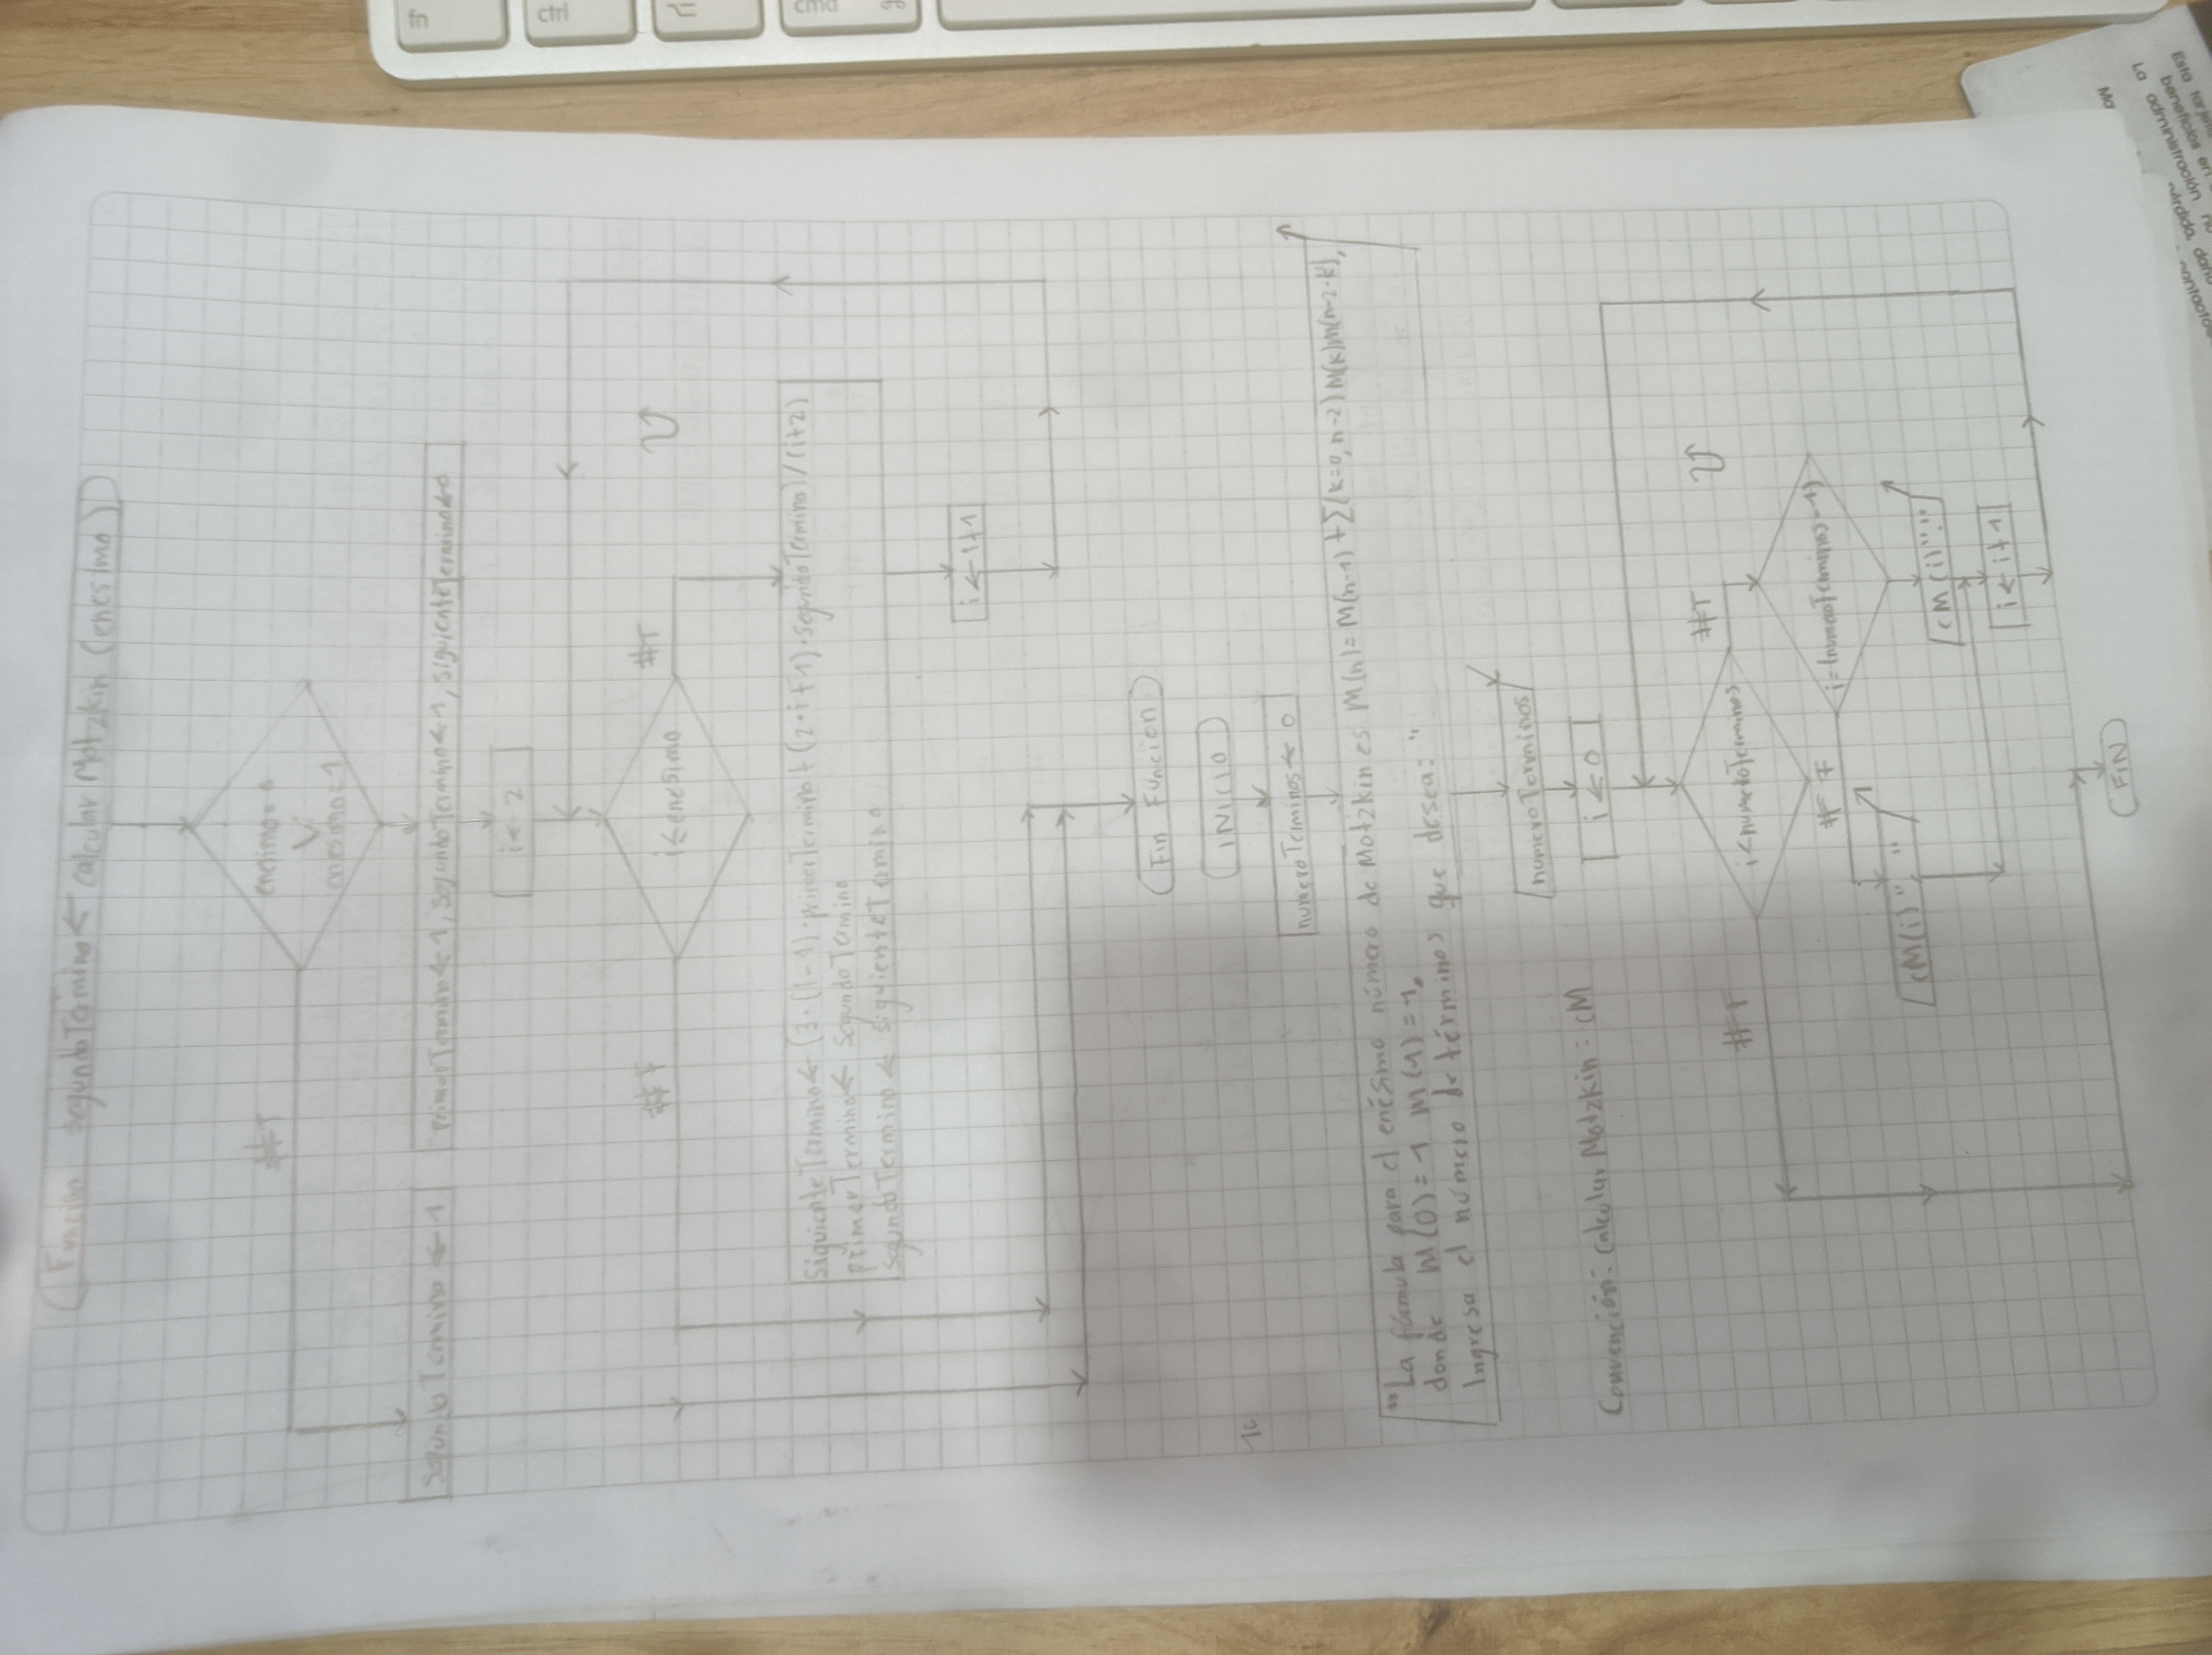
\includegraphics[width=14cm]{dfd/10.jpg}
    \caption{ DFD del punto 10}
    \label{fig: DFD del punto 10}
\end{figure}

\subsubsectionanum{Código}

\importsourcecode[]{c}{code/10.c}{}



\subsection{Punto 11}
	
	Ejemplo de pantalla:
 % Please add the following required packages to your document preamble:
% \usepackage{booktabs}
\begin{lstlisting}
Este programa imprime en pantalla los primeros n terminos de la serie de Triangular.
Esta serie cuenta el número de puntos en una retícula triangular de lado n
Ingrese la cantidad de términos que desea ver: 5

La cantidad 5 de términos de la serie de triangular son: 1, 3, 6, 10, 15
1, 1, 2, 4, 9, 21.
\end{lstlisting}

\begin{lstlisting}
Este programa imprime en pantalla los primeros n terminos de la serie de Triangular.
Esta serie cuenta el número de puntos en una retícula triangular de lado nIngrese la cantidad de términos que desea ver: 9

La cantidad 9 de términos de la serie de triangular son: 1, 3, 6, 10, 15, 21, 28, 36, 45
\end{lstlisting}

\begin{lstlisting}
Este programa imprime en pantalla los primeros n terminos de la serie de Triangular.
Esta serie cuenta el número de puntos en una retícula triangular de lado nIngrese la cantidad de términos que desea ver: 15

La cantidad 15 de términos de la serie de triangular son: 1, 3, 6, 10, 15, 21, 28, 36, 45, 55, 66, 78, 91, 105, 120
\end{lstlisting}

\subsubsectionanum{DFD}
\begin{figure}
    \centering
    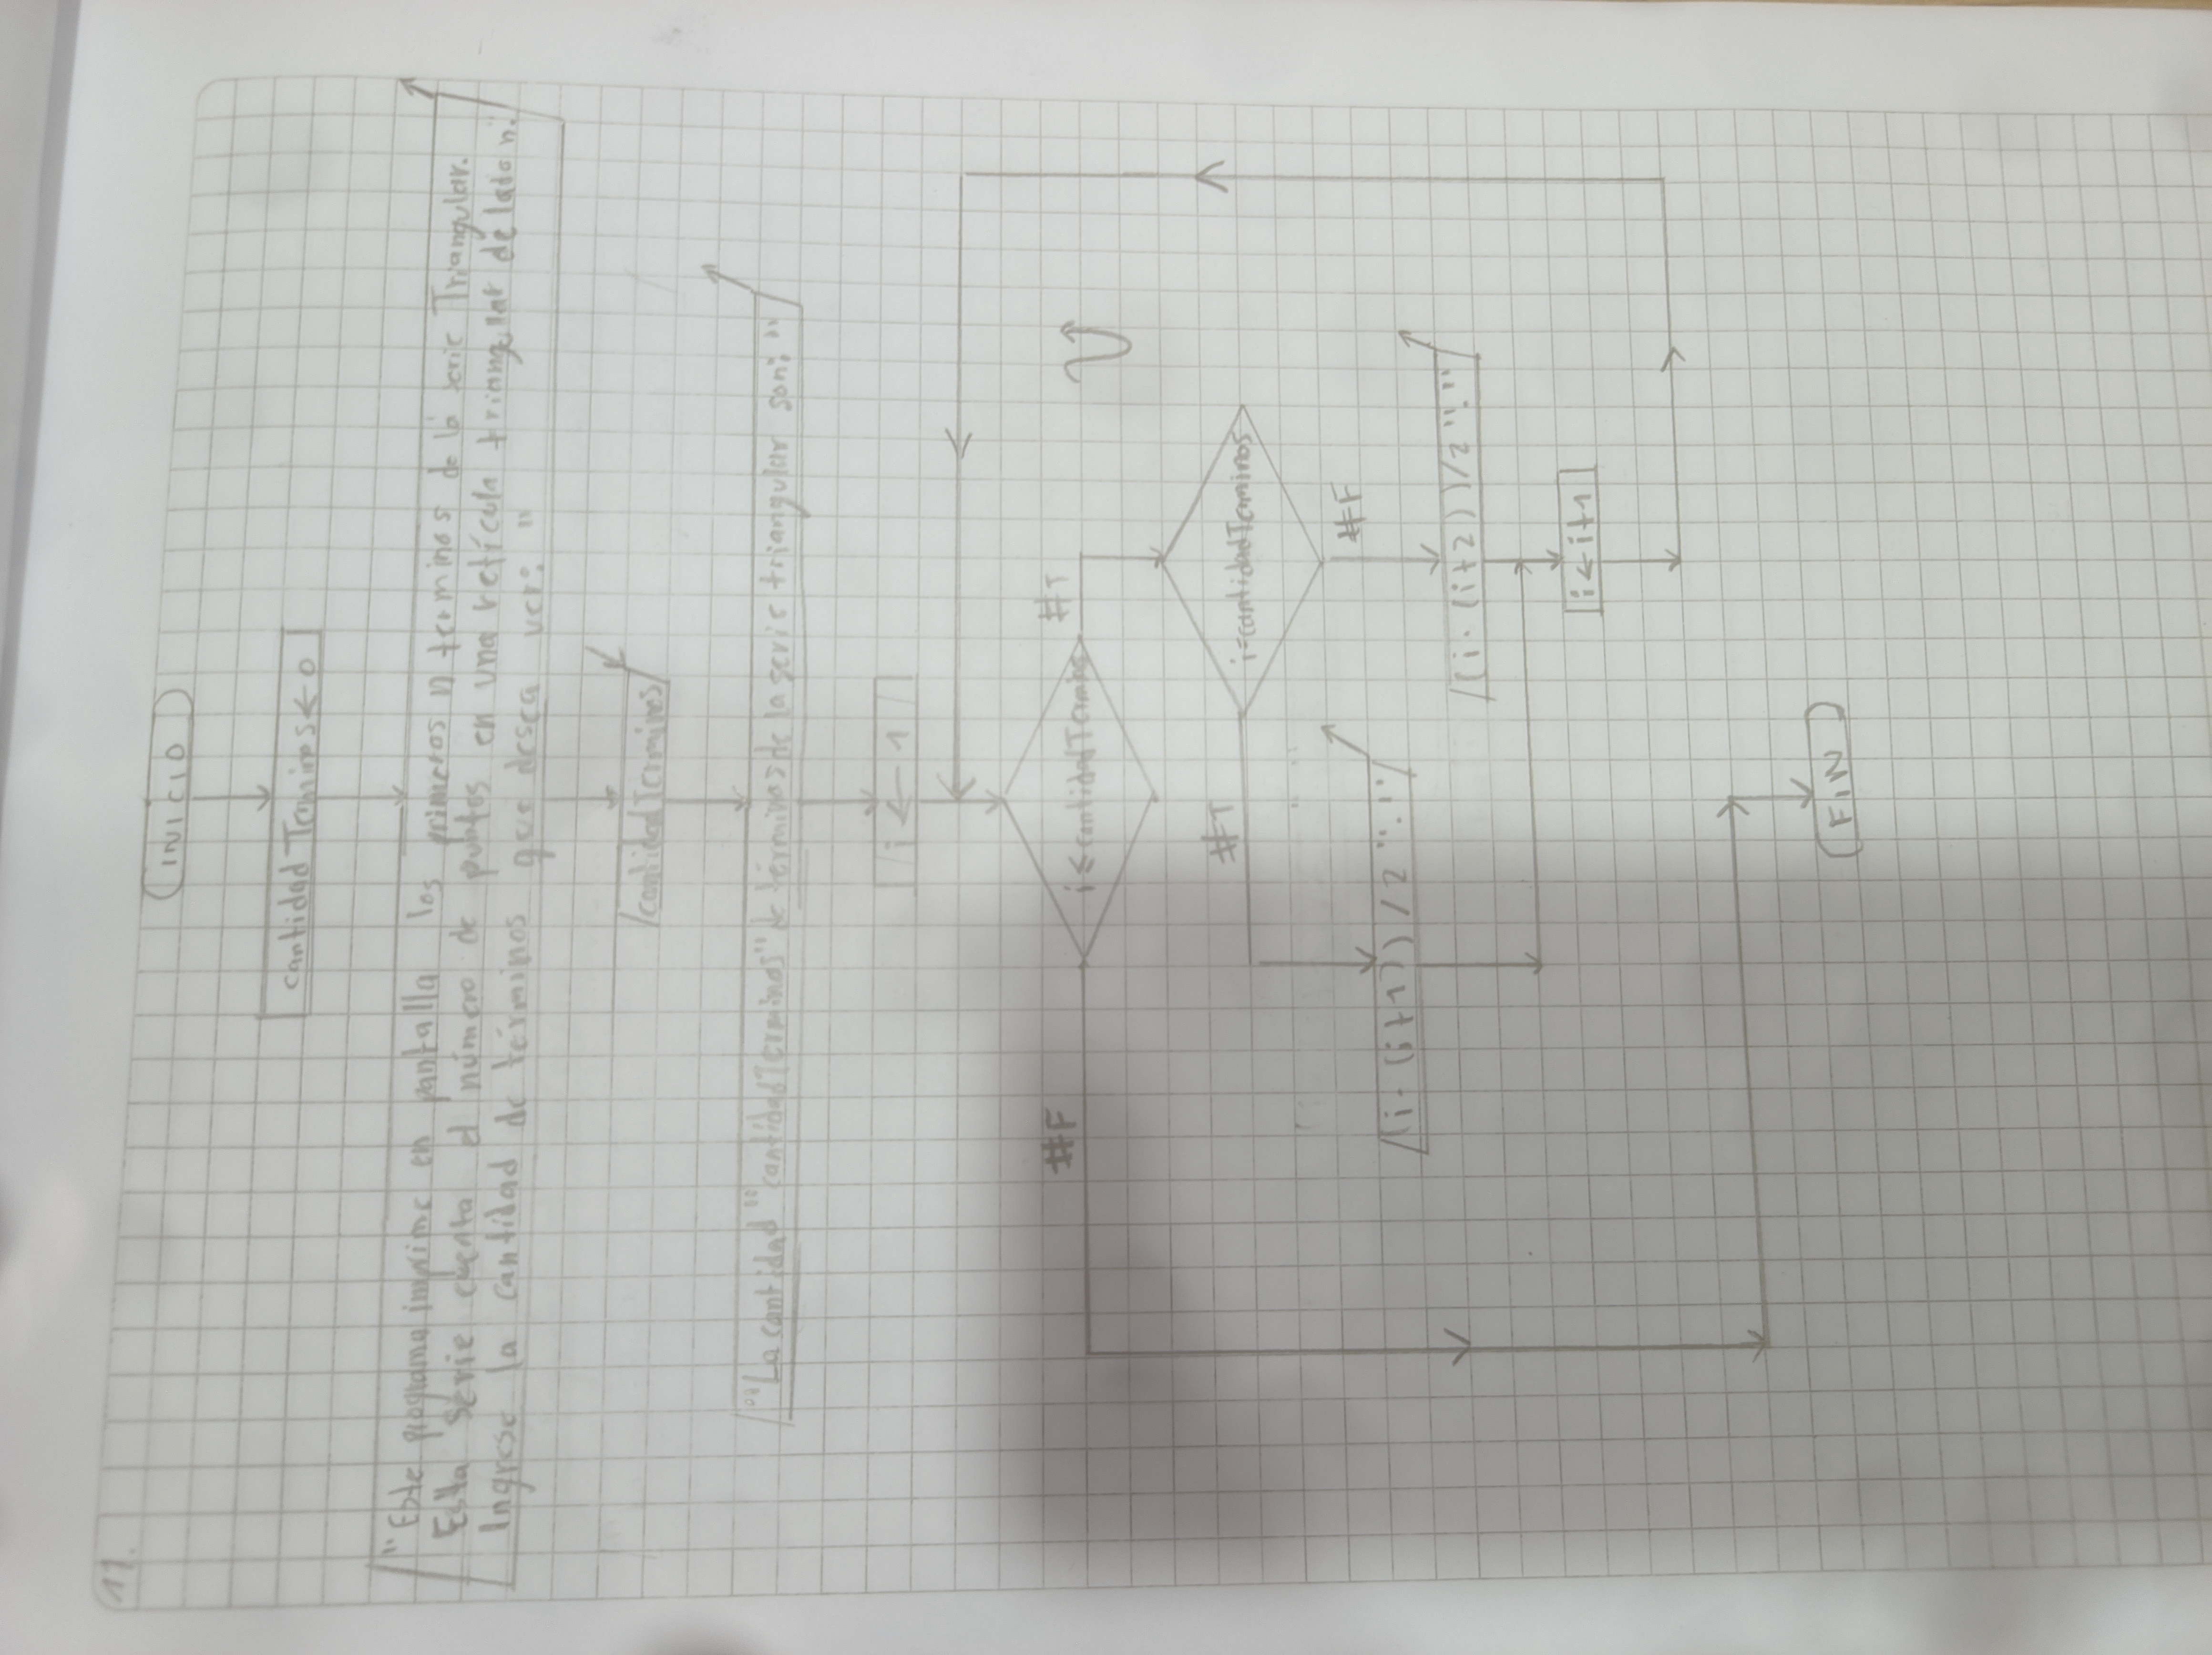
\includegraphics[width=14cm]{dfd/11.jpg}
    \caption{ DFD del punto 11}
    \label{fig: DFD del punto 11}
\end{figure}

\subsubsectionanum{Código}

\importsourcecode[]{c}{code/11.c}{}


\subsection{Punto 12}
	
	Ejemplo de pantalla:
 % Please add the following required packages to your document preamble:
% \usepackage{booktabs}
\begin{lstlisting}
Este programa lee por consola un valor de entrada de tipo número,
y luego imprime este número al reves.
Ingrese el número que desea imprimir al reves: 375

El número 375 impreso al reves es: 573
\end{lstlisting}

\begin{lstlisting}
Este programa lee por consola un valor de entrada de tipo número,
y luego imprime este número al reves.
Ingrese el número que desea imprimir al reves: 987

El número 987 impreso al reves es: 789
\end{lstlisting}

\begin{lstlisting}
Este programa lee por consola un valor de entrada de tipo número,
y luego imprime este número al reves.
Ingrese el número que desea imprimir al reves: 1234567

El número 1234567 impreso al reves es: 7654321
\end{lstlisting}

\subsubsectionanum{DFD}
\begin{figure}
    \centering
    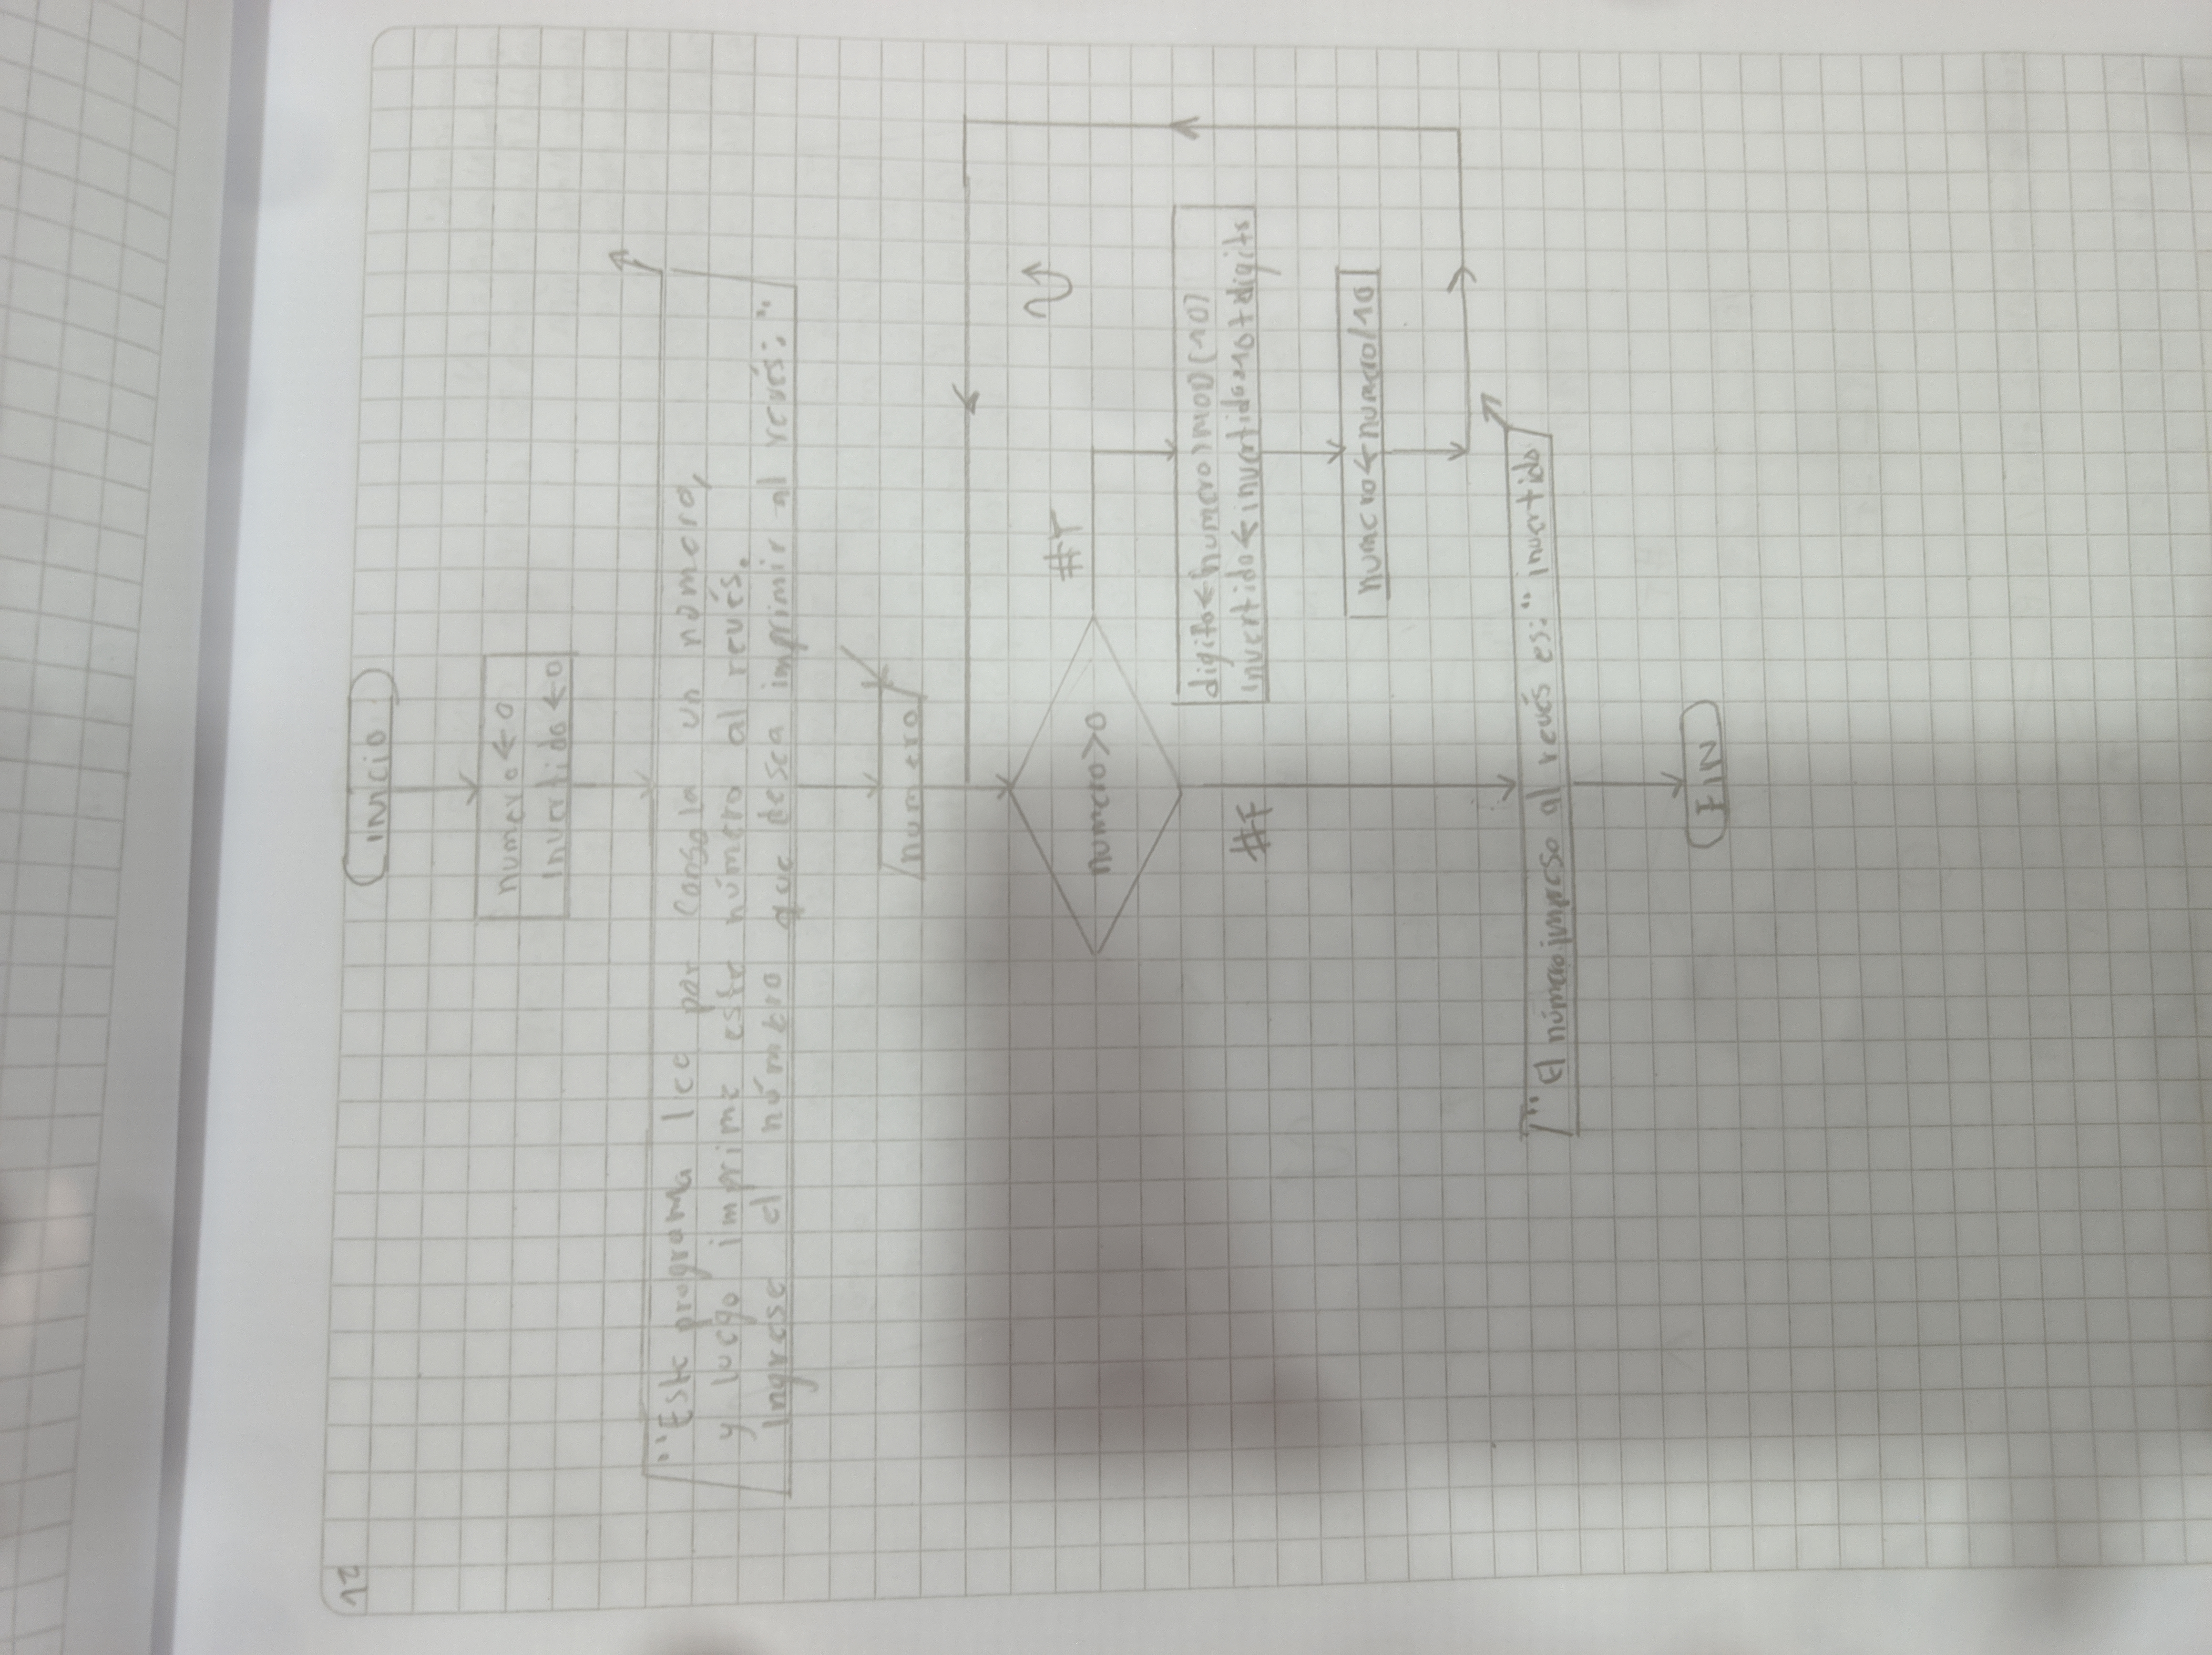
\includegraphics[width=14cm]{dfd/12.jpg}
    \caption{ DFD del punto 12}
    \label{fig: DFD del punto 12}
\end{figure}

\subsubsectionanum{Código}

\importsourcecode[]{c}{code/12.c}{}



\subsection{Punto 13}
	
	Ejemplo de pantalla:
 % Please add the following required packages to your document preamble:
% \usepackage{booktabs}
\begin{lstlisting}
Este programa recibie por consola, 75 números diferentes de cero.
Luego imprime en pantalla la cantidad de números mayores a 150,
número mayor y número menor encontrado en el grupo de números ingresados.
Cantidad de números negativos encontrados en el grupo de números ingresados.
Promedio de los números positivos encontrados.
Ingrese el número 1: 31
Ingrese el número 2: 3423
Ingrese el número 3: 234
Ingrese el número 4: -454
Ingrese el número 5: -3243
Ingrese el número 6: 545
Ingrese el número 7: 3
Ingrese el número 8: 234
Ingrese el número 9: 54
Ingrese el número 10: 45
Ingrese el número 11: 23
Ingrese el número 12: 43
Ingrese el número 13: 454
Ingrese el número 14: 234
Ingrese el número 15: 2
Ingrese el número 16: 54
Ingrese el número 17: 4546
Ingrese el número 18: 76
Ingrese el número 19: 5
Ingrese el número 20: 6
Ingrese el número 21: 6578
Ingrese el número 22: 7
Ingrese el número 23: 6
Ingrese el número 24: -67
Ingrese el número 25: -56
Ingrese el número 26: -76
Ingrese el número 27: 456
Ingrese el número 28: -56
Ingrese el número 29: -65
Ingrese el número 30: 86 
Ingrese el número 31: 967
Ingrese el número 32: -56
Ingrese el número 33: 876
Ingrese el número 34: -56
Ingrese el número 35: 54
Ingrese el número 36: 34
Ingrese el número 37: 47
Ingrese el número 38: 56
Ingrese el número 39: 85
Ingrese el número 40: 89 
Ingrese el número 41: 43
Ingrese el número 42: 234
Ingrese el número 43: 3
Ingrese el número 44: 2
Ingrese el número 45: 343
Ingrese el número 46: 45
Ingrese el número 47: 464
Ingrese el número 48: 4
Ingrese el número 49: 345
Ingrese el número 50: 45
Ingrese el número 51: 56
Ingrese el número 52: 765
Ingrese el número 53: 45
Ingrese el número 54: 56
Ingrese el número 55: -92
Ingrese el número 56: -4325
Ingrese el número 57: 34
Ingrese el número 58: 34
Ingrese el número 59: 53
Ingrese el número 60: 23
Ingrese el número 61: 324
Ingrese el número 62: 123
Ingrese el número 63: 342
Ingrese el número 64: 235
Ingrese el número 65: 634
Ingrese el número 66: 2341
Ingrese el número 67: 43
Ingrese el número 68: 35
Ingrese el número 69: 230
Ingrese el número 70: 5290
Ingrese el número 71: 34
Ingrese el número 72: -553
Ingrese el número 73: -2435
Ingrese el número 74: -34
Ingrese el número 75: 346

Cantidad de números mayores a 150: 24
Número mayor: 6578
Número menor: -4325
Cantidad de números negativos: 14
Promedio de los números positivos: 523.34
\end{lstlisting}

\begin{lstlisting}
Este programa recibie por consola, 75 números diferentes de cero.
Luego imprime en pantalla la cantidad de números mayores a 150,
número mayor y número menor encontrado en el grupo de números ingresados.
Cantidad de números negativos encontrados en el grupo de números ingresados.
Promedio de los números positivos encontrados.

Ingrese el número 1: -100
Ingrese el número 2: 200
Ingrese el número 3: -50
Ingrese el número 4: 0
Ingrese el número 5: 150
Ingrese el número 6: -300
Ingrese el número 7: 1000
Ingrese el número 8: -75
Ingrese el número 9: 500
Ingrese el número 10: -25
Ingrese el número 11: 75
Ingrese el número 12: -200
Ingrese el número 13: 50
Ingrese el número 14: -150
Ingrese el número 15: 25
Ingrese el número 16: 0
Ingrese el número 17: -500
Ingrese el número 18: 300
Ingrese el número 19: -1000
Ingrese el número 20: 2000
Ingrese el número 21: -750
Ingrese el número 22: 10000
Ingrese el número 23: -250
Ingrese el número 24: 750
Ingrese el número 25: -2000
Ingrese el número 26: 1500
Ingrese el número 27: -25
Ingrese el número 28: 50
Ingrese el número 29: -3000
Ingrese el número 30: 75 
Ingrese el número 31: 25
Ingrese el número 32: 10
Ingrese el número 33: -10000
Ingrese el número 34: 20000
Ingrese el número 35: -7500
Ingrese el número 36: 5000
Ingrese el número 37: -2500
Ingrese el número 38: 7500
Ingrese el número 39: -5000
Ingrese el número 40: 2500
Ingrese el número 41: -10
Ingrese el número 42: 100
Ingrese el número 43: -20000
Ingrese el número 44: 30000
Ingrese el número 45: -15000
Ingrese el número 46: 10000
Ingrese el número 47: -5000
Ingrese el número 48: 15000
Ingrese el número 49: -1000
Ingrese el número 50: 5000
Ingrese el número 51: -250
Ingrese el número 52: 750
Ingrese el número 53: -150
Ingrese el número 54: 500
Ingrese el número 55: -100
Ingrese el número 56: 250
Ingrese el número 57: -50
Ingrese el número 58: 100
Ingrese el número 59: -25
Ingrese el número 60: 50
Ingrese el número 61: -5
Ingrese el número 62: 10
Ingrese el número 63: -300
Ingrese el número 64: 500
Ingrese el número 65: -7500
Ingrese el número 66: 1000
Ingrese el número 67: -2000
Ingrese el número 68: 1500
Ingrese el número 69: -500
Ingrese el número 70: 7500
Ingrese el número 71: -10000
Ingrese el número 72: 20000
Ingrese el número 73: -2500
Ingrese el número 74: 10000
Ingrese el número 75: -1000

Cantidad de números mayores a 150: 17
Número mayor: 30000
Número menor: -10000
Cantidad de números negativos: 40
Promedio de los números positivos: 6437.12
\end{lstlisting}

\begin{lstlisting}
Este programa recibie por consola, 75 números diferentes de cero.
Luego imprime en pantalla la cantidad de números mayores a 150,
número mayor y número menor encontrado en el grupo de números ingresados.
Cantidad de números negativos encontrados en el grupo de números ingresados.
Promedio de los números positivos encontrados.

Ingrese el número 1: 10
Ingrese el número 2: 20
Ingrese el número 3: 30
Ingrese el número 4: 40
Ingrese el número 5: 50
Ingrese el número 6: 60
Ingrese el número 7: 70
Ingrese el número 8: 80
Ingrese el número 9: 90
Ingrese el número 10: 100
Ingrese el número 11: 110
Ingrese el número 12: 120
Ingrese el número 13: 130
Ingrese el número 14: 140
Ingrese el número 15: 150
Ingrese el número 16: 160
Ingrese el número 17: 170
Ingrese el número 18: 180
Ingrese el número 19: 190
Ingrese el número 20: 200
Ingrese el número 21: 210
Ingrese el número 22: 220
Ingrese el número 23: 230
Ingrese el número 24: 240
Ingrese el número 25: 250
Ingrese el número 26: 260
Ingrese el número 27: 270
Ingrese el número 28: 280
Ingrese el número 29: 290
Ingrese el número 30: 300
Ingrese el número 31: 310
Ingrese el número 32: 320
Ingrese el número 33: 330
Ingrese el número 34: 340
Ingrese el número 35: 350
Ingrese el número 36: 360
Ingrese el número 37: 370
Ingrese el número 38: 380
Ingrese el número 39: 390
Ingrese el número 40: 400
Ingrese el número 41: 410
Ingrese el número 42: 420
Ingrese el número 43: 430
Ingrese el número 44: 440
Ingrese el número 45: 450
Ingrese el número 46: 460
Ingrese el número 47: 470
Ingrese el número 48: 480
Ingrese el número 49: 490
Ingrese el número 50: 500
Ingrese el número 51: 510
Ingrese el número 52: 520
Ingrese el número 53: 530
Ingrese el número 54: 540
Ingrese el número 55: 550
Ingrese el número 56: 560
Ingrese el número 57: 570
Ingrese el número 58: 580
Ingrese el número 59: 590
Ingrese el número 60: 600
Ingrese el número 61: 610
Ingrese el número 62: 620
Ingrese el número 63: 630
Ingrese el número 64: 640
Ingrese el número 65: 650
Ingrese el número 66: 660
Ingrese el número 67: 670
Ingrese el número 68: 680
Ingrese el número 69: 690
Ingrese el número 70: 700
Ingrese el número 71: 710
Ingrese el número 72: 720
Ingrese el número 73: 730
Ingrese el número 74: 740
Ingrese el número 75: 750

Cantidad de números mayores a 150: 26
Número mayor: 750
Número menor: 10
Cantidad de números negativos: 0
Promedio de los números positivos: 380.77
\end{lstlisting}


\subsubsectionanum{DFD}
\begin{figure}
    \centering
    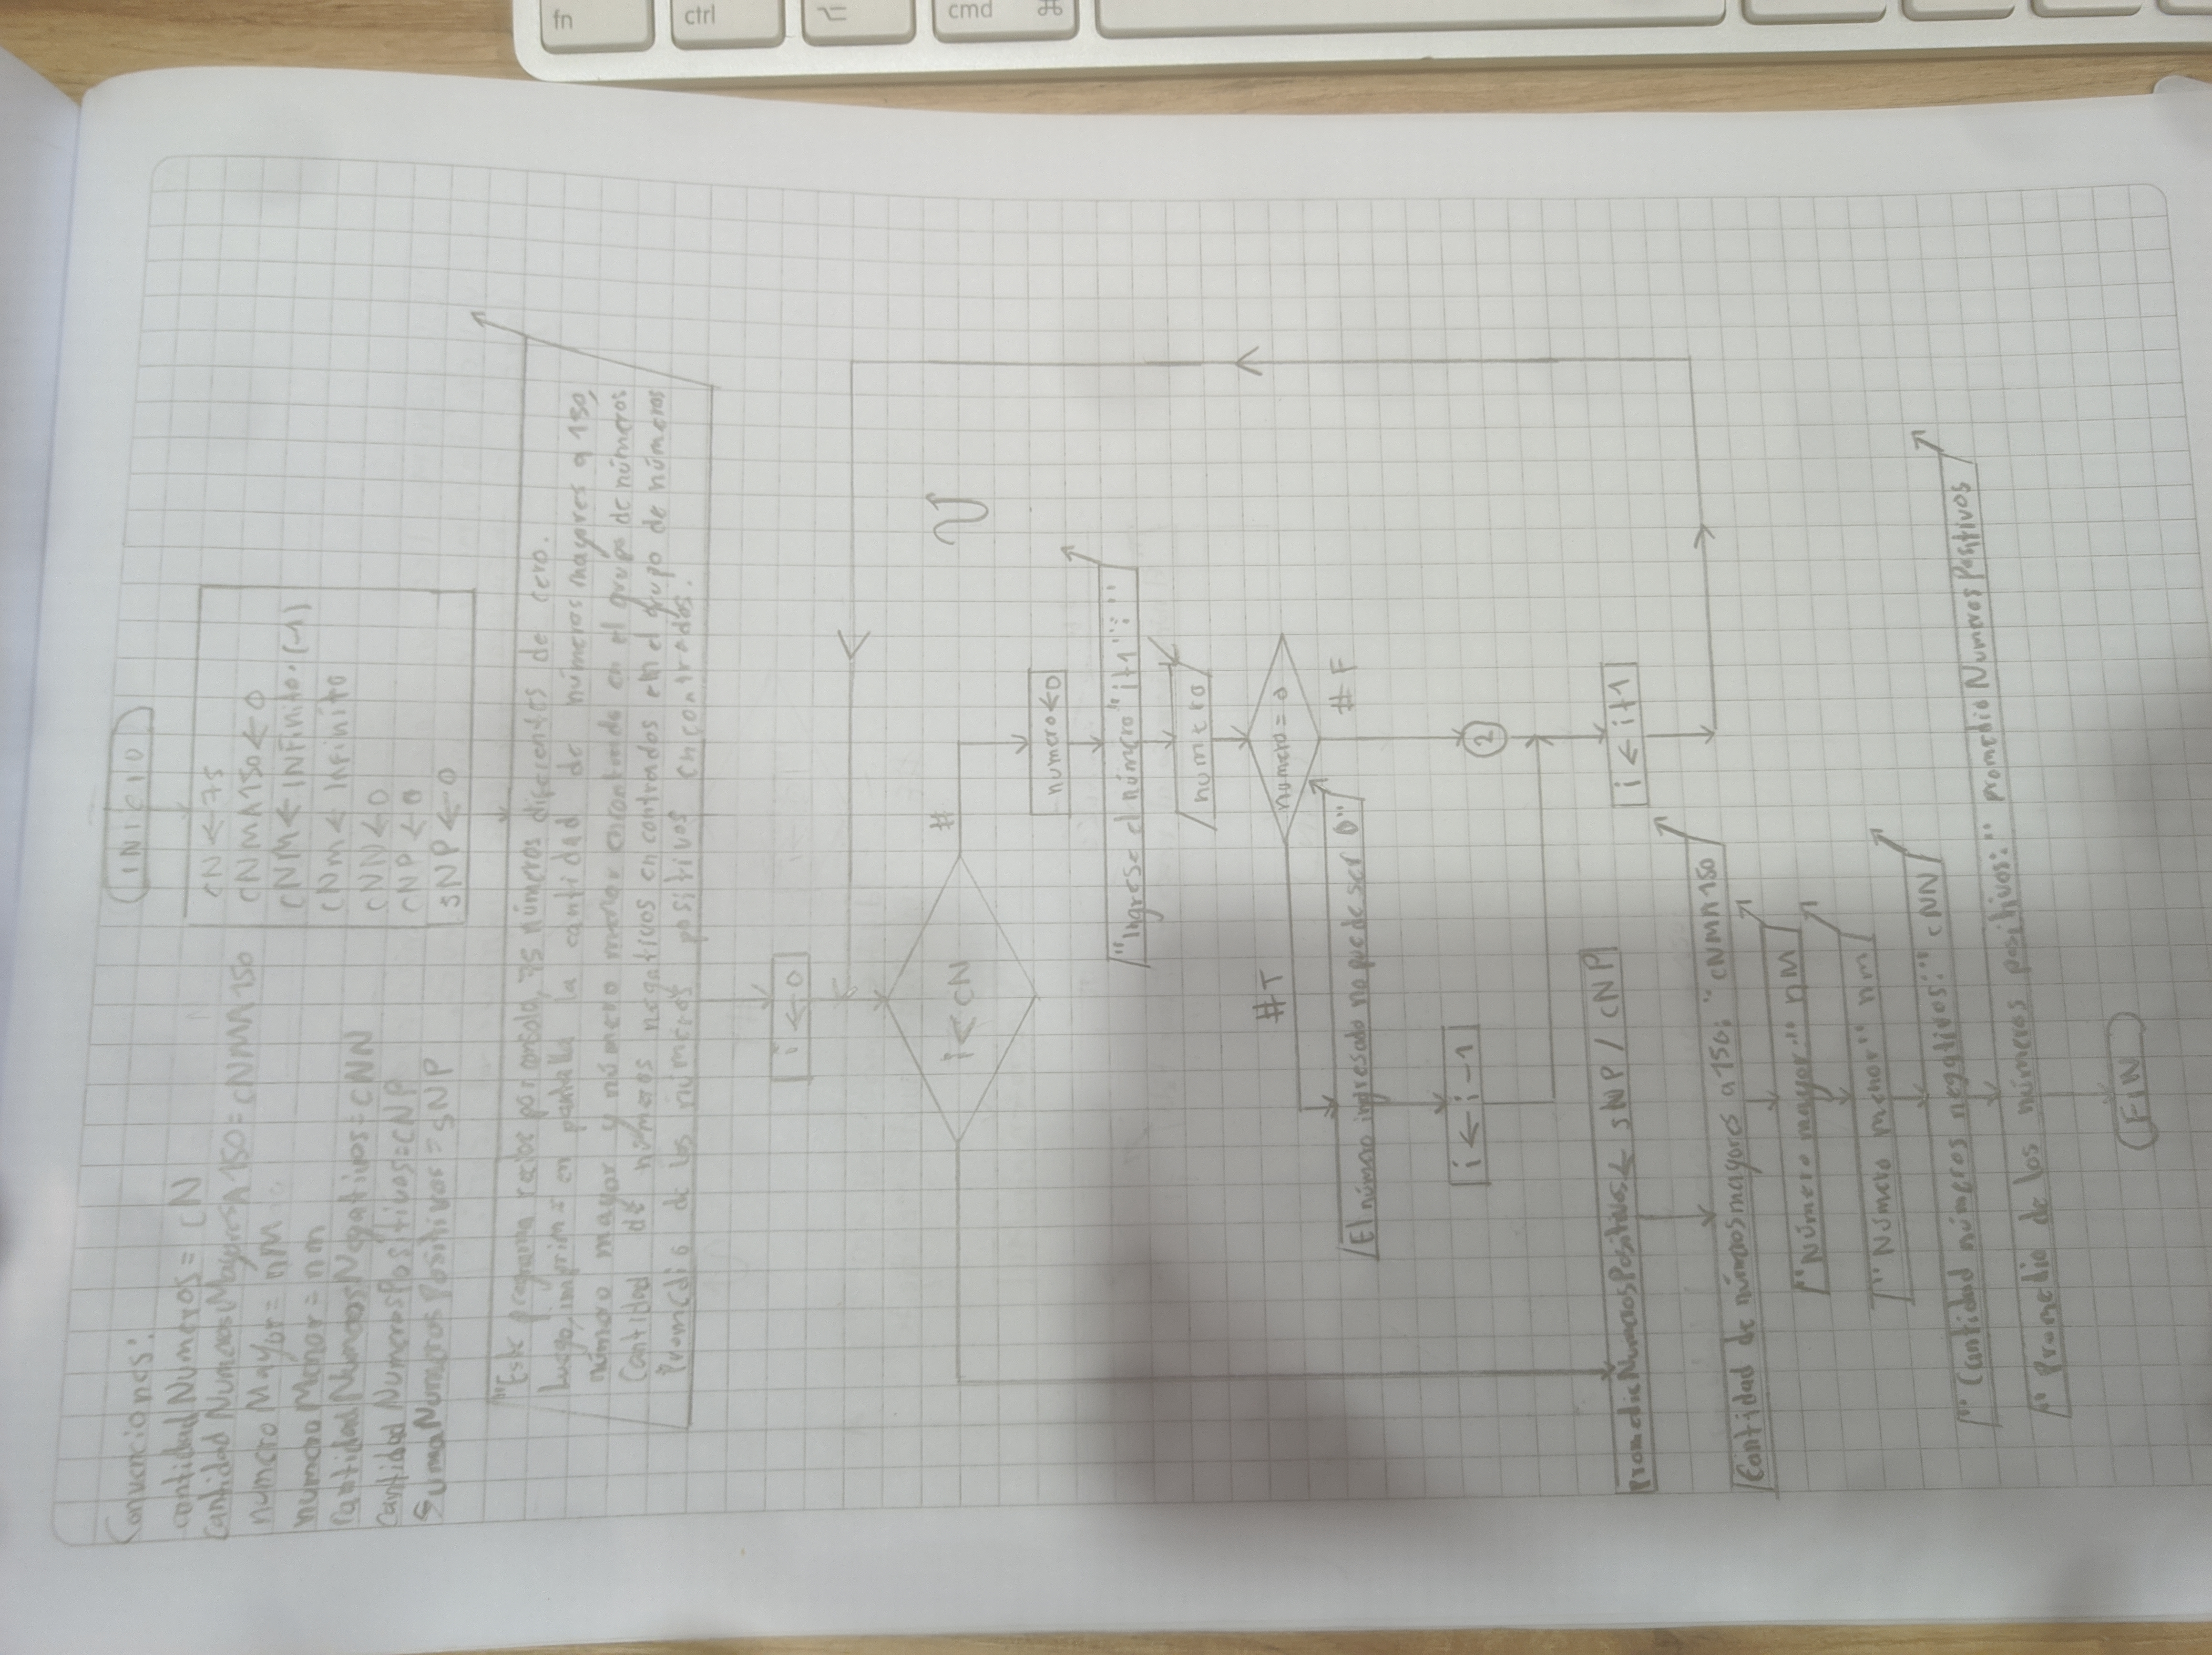
\includegraphics[width=14cm]{dfd/13.jpg}
    \caption{ DFD del punto 13}
    \label{fig: DFD del punto 13}
\end{figure}

\subsubsectionanum{Código}

\importsourcecode[]{c}{code/13.c}{}



\subsection{Punto 14}
	
	Ejemplo de pantalla:
 % Please add the following required packages to your document preamble:
% \usepackage{booktabs}
\begin{lstlisting}
1 x 1 = 1
1 x 2 = 2
1 x 3 = 3
1 x 4 = 4
1 x 5 = 5
1 x 6 = 6
1 x 7 = 7
1 x 8 = 8
1 x 9 = 9
1 x 10 = 10

2 x 1 = 2
2 x 2 = 4
2 x 3 = 6
2 x 4 = 8
2 x 5 = 10
2 x 6 = 12
2 x 7 = 14
2 x 8 = 16
2 x 9 = 18
2 x 10 = 20

3 x 1 = 3
3 x 2 = 6
3 x 3 = 9
3 x 4 = 12
3 x 5 = 15
3 x 6 = 18
3 x 7 = 21
3 x 8 = 24
3 x 9 = 27
3 x 10 = 30

4 x 1 = 4
4 x 2 = 8
4 x 3 = 12
4 x 4 = 16
4 x 5 = 20
4 x 6 = 24
4 x 7 = 28
4 x 8 = 32
4 x 9 = 36
4 x 10 = 40

5 x 1 = 5
5 x 2 = 10
5 x 3 = 15
5 x 4 = 20
5 x 5 = 25
5 x 6 = 30
5 x 7 = 35
5 x 8 = 40
5 x 9 = 45
5 x 10 = 50

6 x 1 = 6
6 x 2 = 12
6 x 3 = 18
6 x 4 = 24
6 x 5 = 30
6 x 6 = 36
6 x 7 = 42
6 x 8 = 48
6 x 9 = 54
6 x 10 = 60

7 x 1 = 7
7 x 2 = 14
7 x 3 = 21
7 x 4 = 28
7 x 5 = 35
7 x 6 = 42
7 x 7 = 49
7 x 8 = 56
7 x 9 = 63
7 x 10 = 70

8 x 1 = 8
8 x 2 = 16
8 x 3 = 24
8 x 4 = 32
8 x 5 = 40
8 x 6 = 48
8 x 7 = 56
8 x 8 = 64
8 x 9 = 72
8 x 10 = 80

9 x 1 = 9
9 x 2 = 18
9 x 3 = 27
9 x 4 = 36
9 x 5 = 45
9 x 6 = 54
9 x 7 = 63
9 x 8 = 72
9 x 9 = 81
9 x 10 = 90

10 x 1 = 10
10 x 2 = 20
10 x 3 = 30
10 x 4 = 40
10 x 5 = 50
10 x 6 = 60
10 x 7 = 70
10 x 8 = 80
10 x 9 = 90
10 x 10 = 100
\end{lstlisting}

\begin{lstlisting}
1 x 1 = 1
1 x 2 = 2
1 x 3 = 3
1 x 4 = 4
1 x 5 = 5
1 x 6 = 6
1 x 7 = 7
1 x 8 = 8
1 x 9 = 9
1 x 10 = 10

2 x 1 = 2
2 x 2 = 4
2 x 3 = 6
2 x 4 = 8
2 x 5 = 10
2 x 6 = 12
2 x 7 = 14
2 x 8 = 16
2 x 9 = 18
2 x 10 = 20

3 x 1 = 3
3 x 2 = 6
3 x 3 = 9
3 x 4 = 12
3 x 5 = 15
3 x 6 = 18
3 x 7 = 21
3 x 8 = 24
3 x 9 = 27
3 x 10 = 30

4 x 1 = 4
4 x 2 = 8
4 x 3 = 12
4 x 4 = 16
4 x 5 = 20
4 x 6 = 24
4 x 7 = 28
4 x 8 = 32
4 x 9 = 36
4 x 10 = 40

5 x 1 = 5
5 x 2 = 10
5 x 3 = 15
5 x 4 = 20
5 x 5 = 25
5 x 6 = 30
5 x 7 = 35
5 x 8 = 40
5 x 9 = 45
5 x 10 = 50

6 x 1 = 6
6 x 2 = 12
6 x 3 = 18
6 x 4 = 24
6 x 5 = 30
6 x 6 = 36
6 x 7 = 42
6 x 8 = 48
6 x 9 = 54
6 x 10 = 60

7 x 1 = 7
7 x 2 = 14
7 x 3 = 21
7 x 4 = 28
7 x 5 = 35
7 x 6 = 42
7 x 7 = 49
7 x 8 = 56
7 x 9 = 63
7 x 10 = 70

8 x 1 = 8
8 x 2 = 16
8 x 3 = 24
8 x 4 = 32
8 x 5 = 40
8 x 6 = 48
8 x 7 = 56
8 x 8 = 64
8 x 9 = 72
8 x 10 = 80

9 x 1 = 9
9 x 2 = 18
9 x 3 = 27
9 x 4 = 36
9 x 5 = 45
9 x 6 = 54
9 x 7 = 63
9 x 8 = 72
9 x 9 = 81
9 x 10 = 90

10 x 1 = 10
10 x 2 = 20
10 x 3 = 30
10 x 4 = 40
10 x 5 = 50
10 x 6 = 60
10 x 7 = 70
10 x 8 = 80
10 x 9 = 90
10 x 10 = 100
\end{lstlisting}

\begin{lstlisting}
1 x 1 = 1
1 x 2 = 2
1 x 3 = 3
1 x 4 = 4
1 x 5 = 5
1 x 6 = 6
1 x 7 = 7
1 x 8 = 8
1 x 9 = 9
1 x 10 = 10

2 x 1 = 2
2 x 2 = 4
2 x 3 = 6
2 x 4 = 8
2 x 5 = 10
2 x 6 = 12
2 x 7 = 14
2 x 8 = 16
2 x 9 = 18
2 x 10 = 20

3 x 1 = 3
3 x 2 = 6
3 x 3 = 9
3 x 4 = 12
3 x 5 = 15
3 x 6 = 18
3 x 7 = 21
3 x 8 = 24
3 x 9 = 27
3 x 10 = 30

4 x 1 = 4
4 x 2 = 8
4 x 3 = 12
4 x 4 = 16
4 x 5 = 20
4 x 6 = 24
4 x 7 = 28
4 x 8 = 32
4 x 9 = 36
4 x 10 = 40

5 x 1 = 5
5 x 2 = 10
5 x 3 = 15
5 x 4 = 20
5 x 5 = 25
5 x 6 = 30
5 x 7 = 35
5 x 8 = 40
5 x 9 = 45
5 x 10 = 50

6 x 1 = 6
6 x 2 = 12
6 x 3 = 18
6 x 4 = 24
6 x 5 = 30
6 x 6 = 36
6 x 7 = 42
6 x 8 = 48
6 x 9 = 54
6 x 10 = 60

7 x 1 = 7
7 x 2 = 14
7 x 3 = 21
7 x 4 = 28
7 x 5 = 35
7 x 6 = 42
7 x 7 = 49
7 x 8 = 56
7 x 9 = 63
7 x 10 = 70

8 x 1 = 8
8 x 2 = 16
8 x 3 = 24
8 x 4 = 32
8 x 5 = 40
8 x 6 = 48
8 x 7 = 56
8 x 8 = 64
8 x 9 = 72
8 x 10 = 80

9 x 1 = 9
9 x 2 = 18
9 x 3 = 27
9 x 4 = 36
9 x 5 = 45
9 x 6 = 54
9 x 7 = 63
9 x 8 = 72
9 x 9 = 81
9 x 10 = 90

10 x 1 = 10
10 x 2 = 20
10 x 3 = 30
10 x 4 = 40
10 x 5 = 50
10 x 6 = 60
10 x 7 = 70
10 x 8 = 80
10 x 9 = 90
10 x 10 = 100
\end{lstlisting}

\subsubsectionanum{DFD}
\begin{figure}
    \centering
    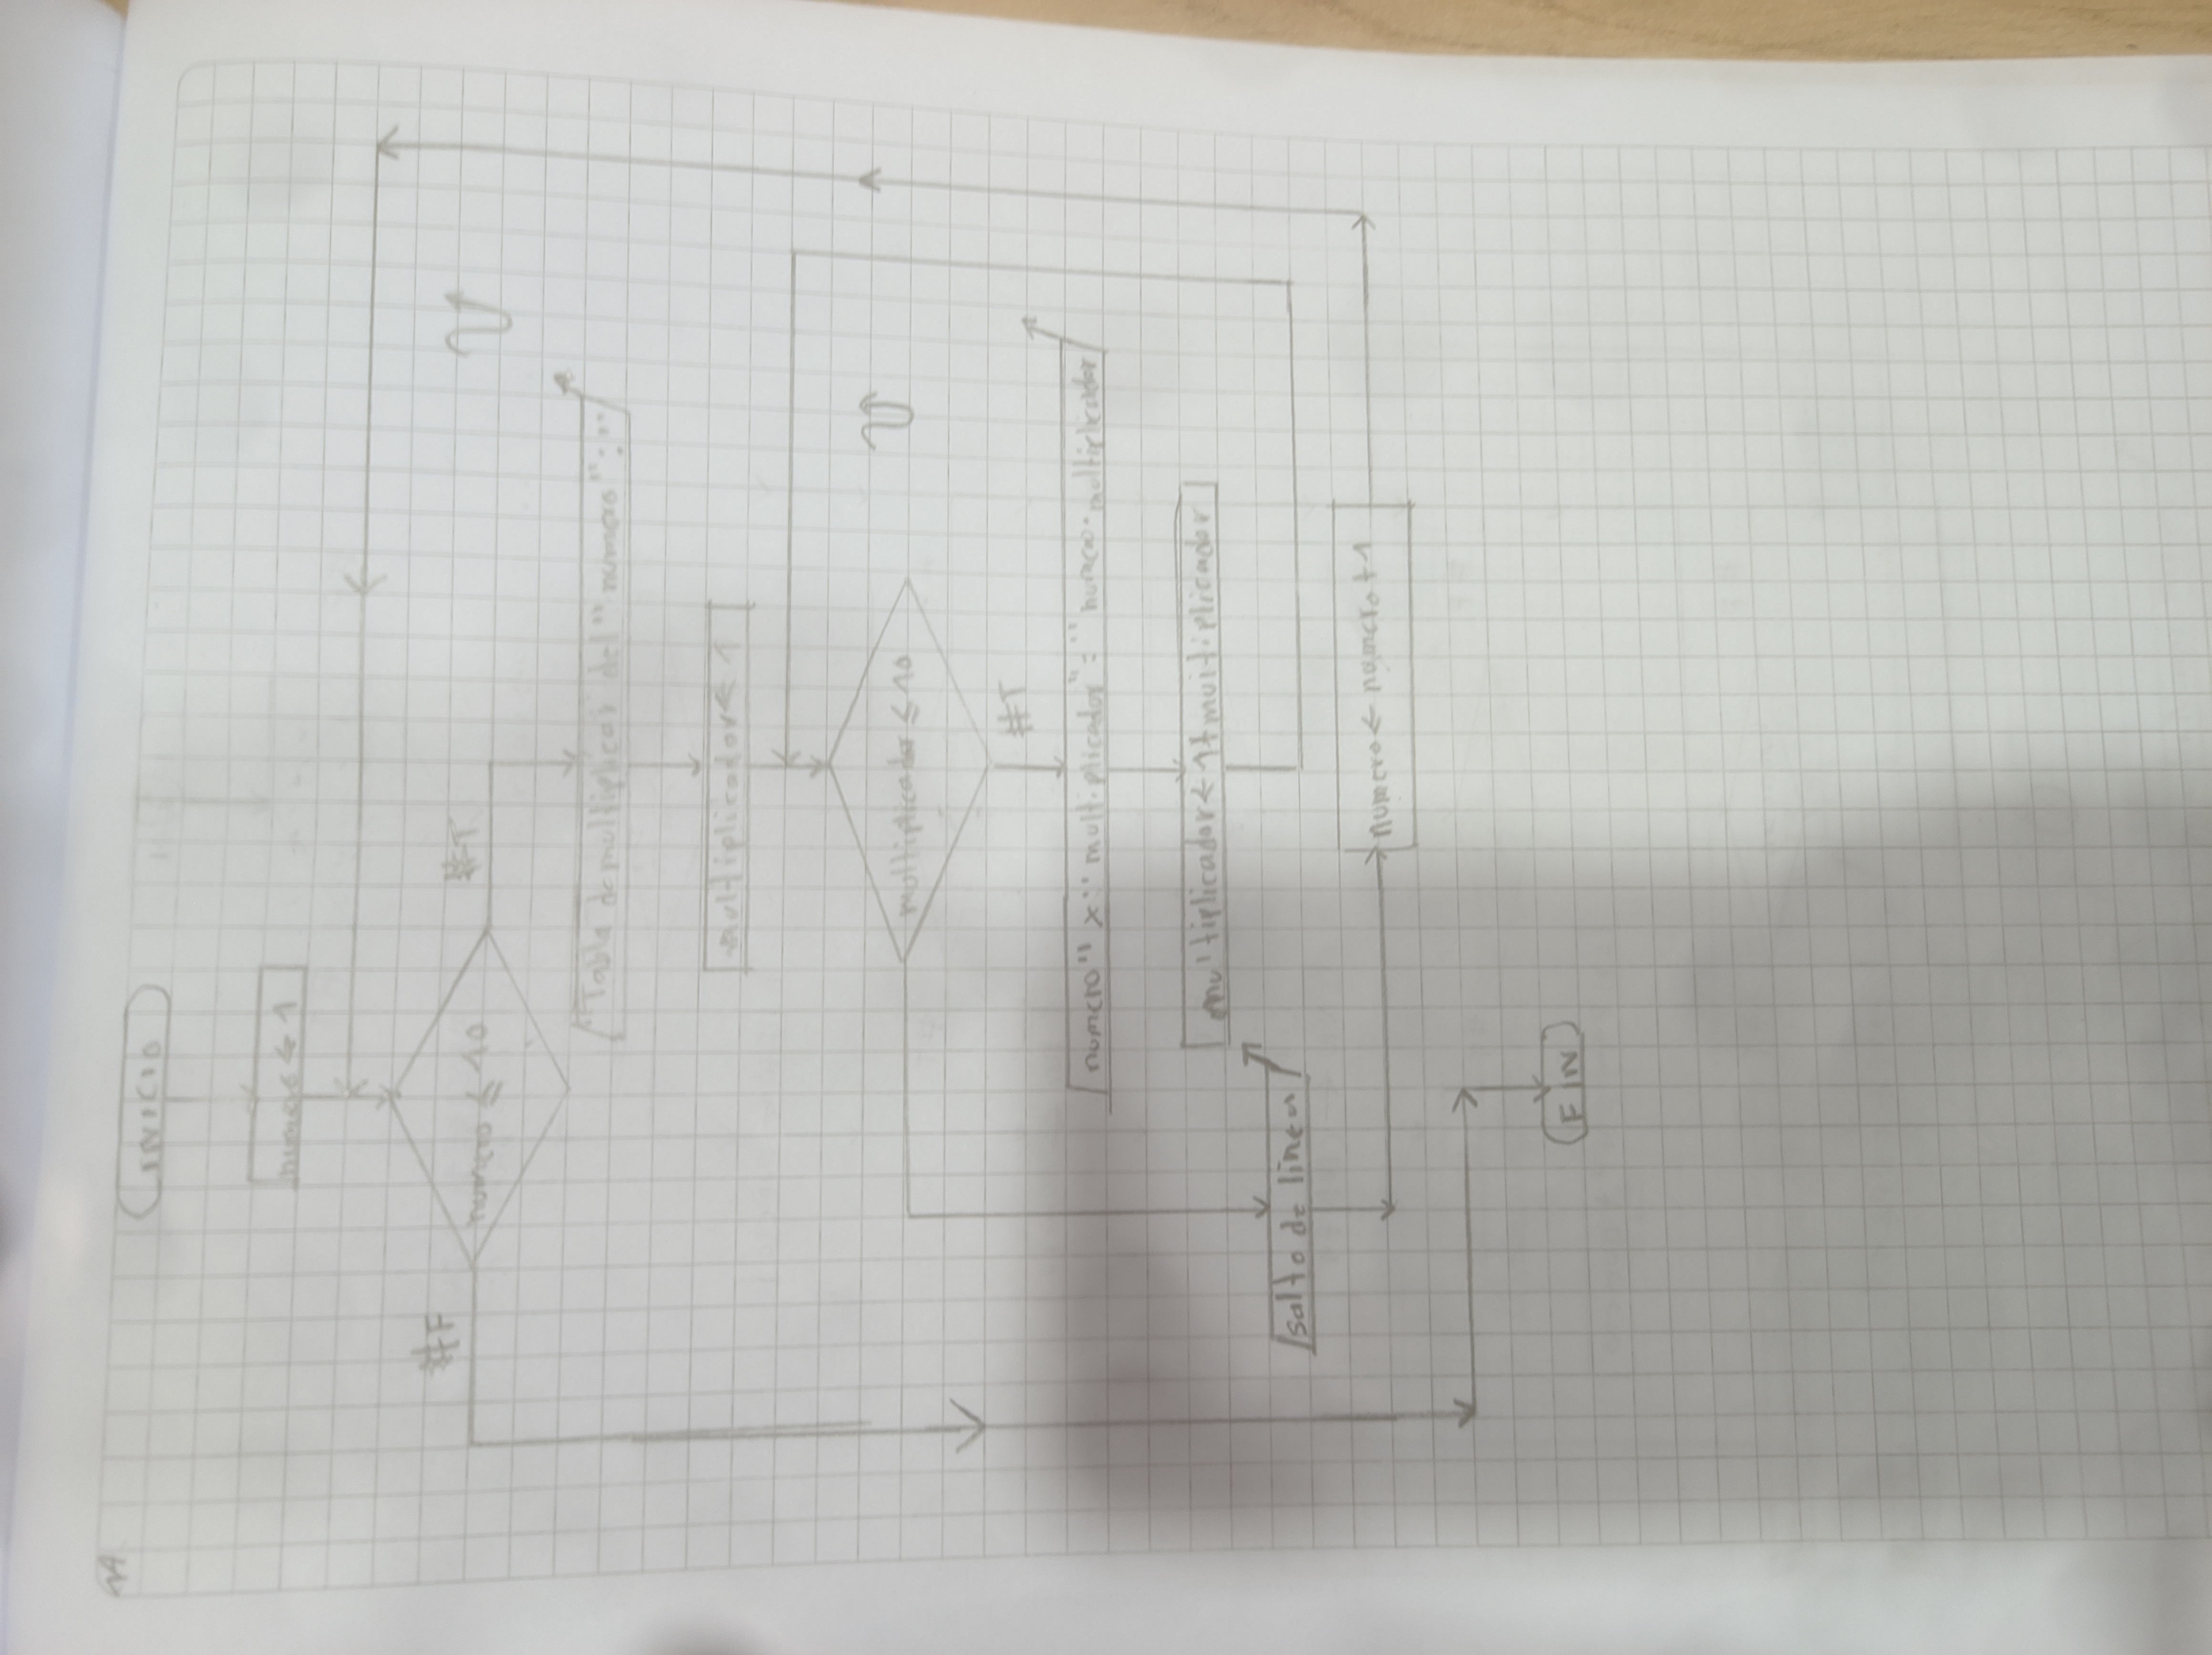
\includegraphics[width=14cm]{dfd/14.jpg}
    \caption{ DFD del punto 14}
    \label{fig: DFD del punto 14}
\end{figure}


\subsubsectionanum{Código}

\importsourcecode[]{c}{code/14.c}{}

\subsection{Punto 15}
	
	Ejemplo de pantalla:
 % Please add the following required packages to your document preamble:
% \usepackage{booktabs}
\begin{lstlisting}
Este programa recibe un número entero positivo como entrada
y luego imprime su factorial.
Ingrese el número que desea calcular su factorial: 5

5! = 120
\end{lstlisting}

\begin{lstlisting}
Este programa recibe un número entero positivo como entrada
y luego imprime su factorial.
Ingrese el número que desea calcular su factorial: 7

7! = 5040
\end{lstlisting}

\begin{lstlisting}
Este programa recibe un número entero positivo como entrada
y luego imprime su factorial.
Ingrese el número que desea calcular su factorial: 2

2! = 2
\end{lstlisting}

\subsubsectionanum{DFD}
\begin{figure}
    \centering
    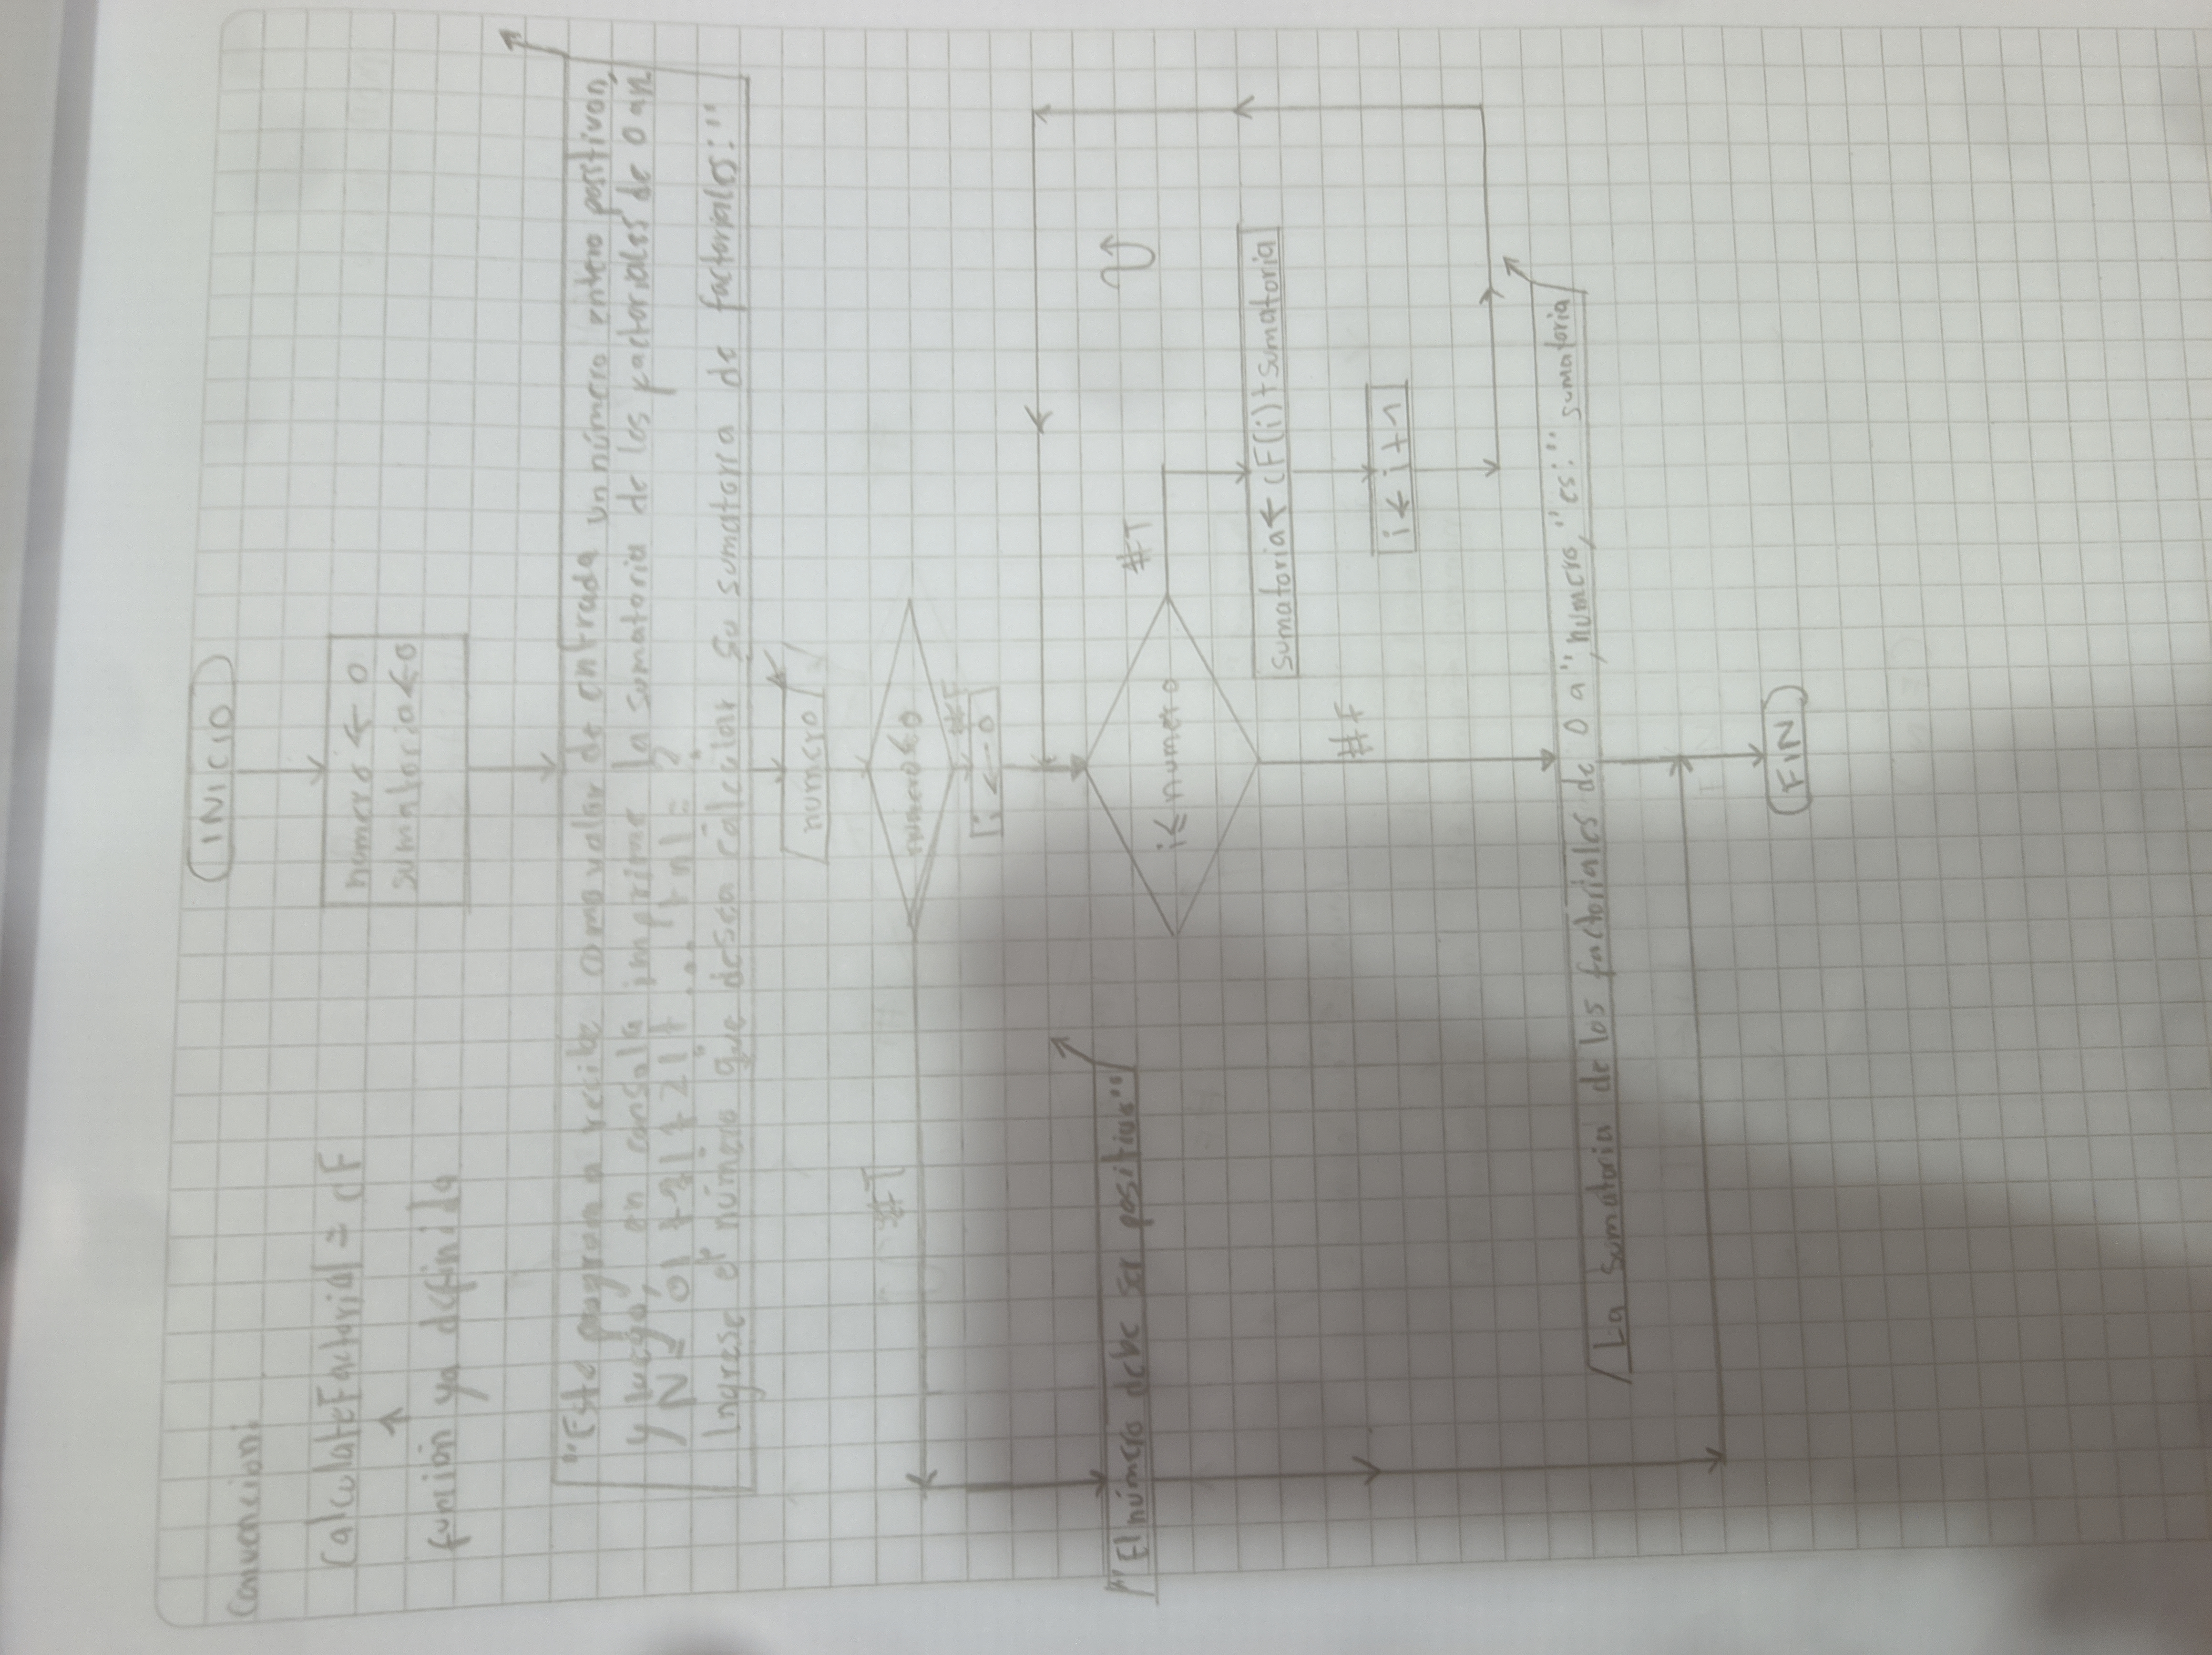
\includegraphics[width=14cm]{dfd/15.jpg}
    \caption{ DFD del punto 15}
    \label{fig: DFD del punto 15}
\end{figure}

\subsubsectionanum{Código}

\importsourcecode[]{c}{code/15.c}{}


\subsection{Punto 16}
	
	Ejemplo de pantalla:
 % Please add the following required packages to your document preamble:
% \usepackage{booktabs}
\begin{lstlisting}
Este programa recibe como valor de entrada un número entero positivo n,
y luego, en consola imprime la sumatoría de los factoriales de 0 a n.
N = 0! + 1! + 2! + ... + n! = ?
Ingrese el número que desea calcular su sumatoria de factoriales: 5
0! + 1! + 2! + 3! + 4! + 5! = 154
\end{lstlisting}

\begin{lstlisting}
Este programa recibe como valor de entrada un número entero positivo n,
y luego, en consola imprime la sumatoría de los factoriales de 0 a n.
N = 0! + 1! + 2! + ... + n! = ?
Ingrese el número que desea calcular su sumatoria de factoriales: 4
0! + 1! + 2! + 3! + 4! = 34
\end{lstlisting}

\begin{lstlisting}
Este programa recibe como valor de entrada un número entero positivo n,
y luego, en consola imprime la sumatoría de los factoriales de 0 a n.
N = 0! + 1! + 2! + ... + n! = ?
Ingrese el número que desea calcular su sumatoria de factoriales: 8
0! + 1! + 2! + 3! + 4! + 5! + 6! + 7! + 8! = 46234
\end{lstlisting}

\subsubsectionanum{DFD}
\begin{figure}
    \centering
    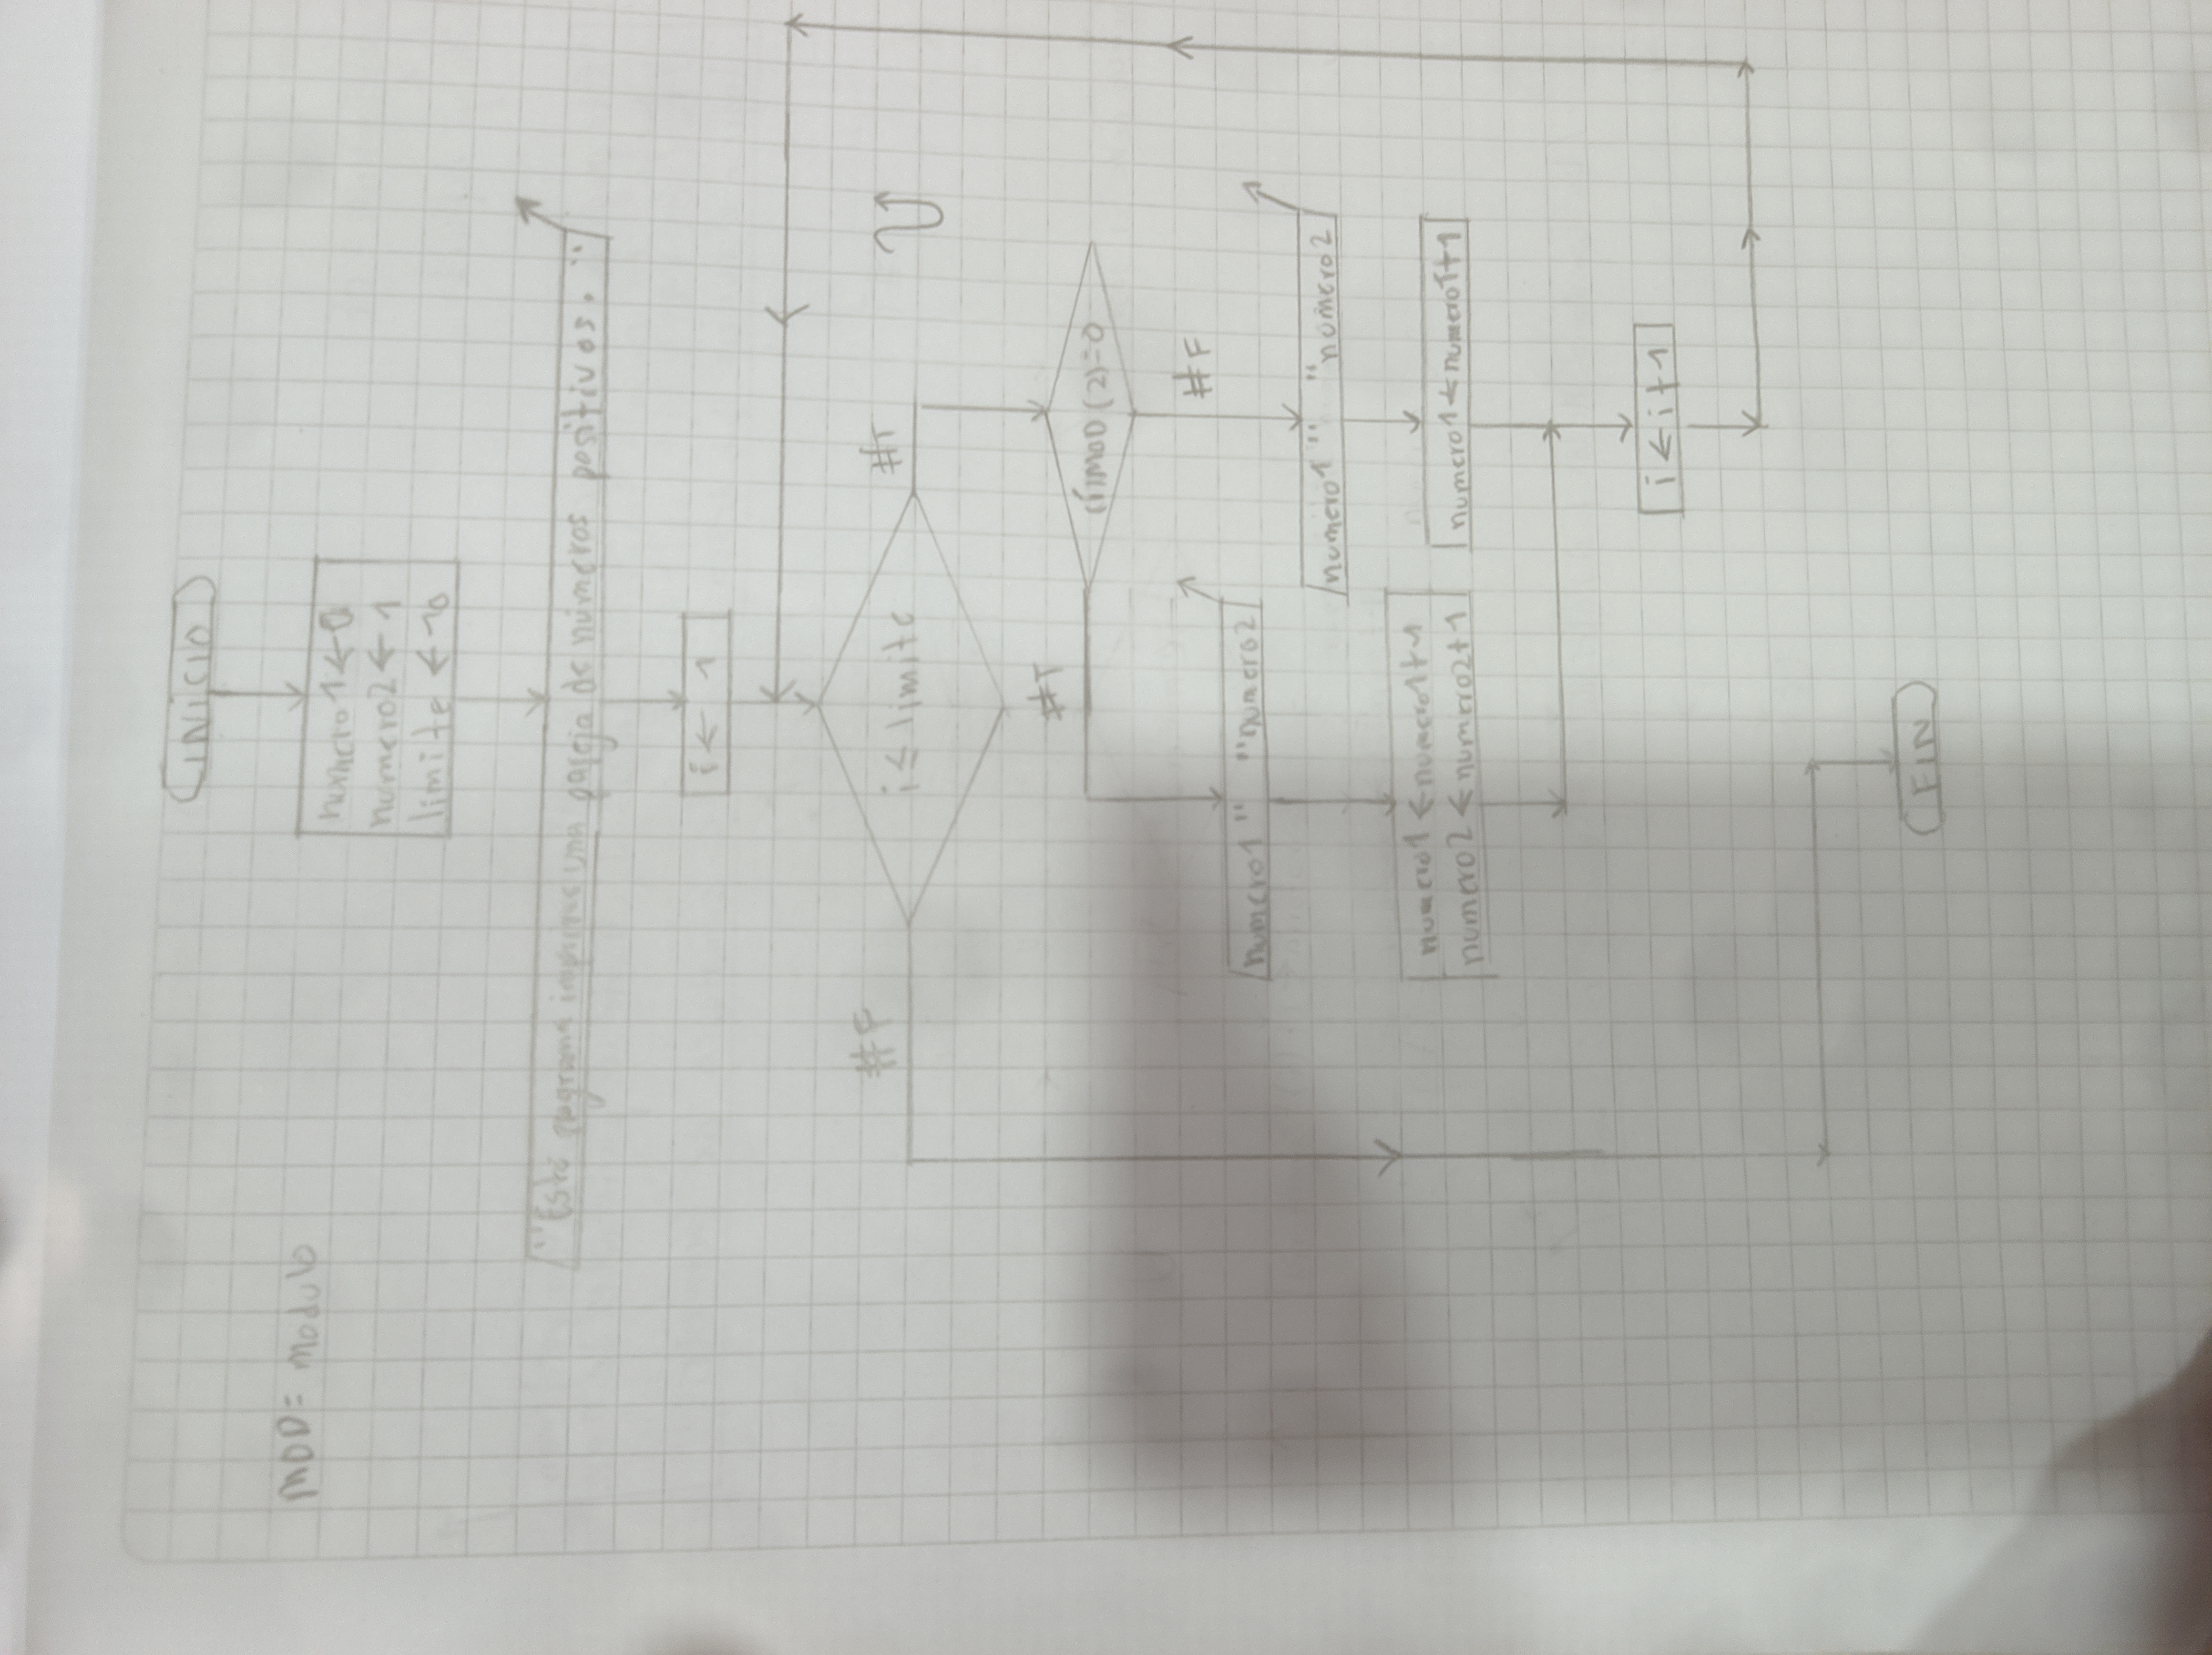
\includegraphics[width=14cm]{dfd/16.jpg}
    \caption{ DFD del punto 16}
    \label{fig: DFD del punto 16}
\end{figure}


\subsubsectionanum{Código}

\importsourcecode[]{c}{code/16.c}{}



\subsection{Punto 17}
	
	Ejemplo de pantalla:
 % Please add the following required packages to your document preamble:
% \usepackage{booktabs}
\begin{lstlisting}
Este programa imprime en pantalla una pareja de números enteros positivos.

0 1
1 1
2 3
3 3
4 5
5 5
6 7
7 7
8 9
9 9
\end{lstlisting}

\begin{lstlisting}
Este programa imprime en pantalla una pareja de números enteros positivos.

0 1
1 1
2 3
3 3
4 5
5 5
6 7
7 7
8 9
9 9
\end{lstlisting}

\begin{lstlisting}
Este programa imprime en pantalla una pareja de números enteros positivos.

0 1
1 1
2 3
3 3
4 5
5 5
6 7
7 7
8 9
9 9
\end{lstlisting}

\subsubsectionanum{Código}

\importsourcecode[]{c}{code/17.c}{}


\subsection{Punto 18}
	
	Ejemplo de pantalla:
 % Please add the following required packages to your document preamble:
% \usepackage{booktabs}
\begin{lstlisting}
Este programa imprime por consola 3 filas de números enteros positivos, cada fila con 9 números.

1 1 1
2 1 2
3 1 3
4 2 1
5 2 2
6 2 3
7 3 1
8 3 2
9 3 3
\end{lstlisting}

\begin{lstlisting}
Este programa imprime por consola 3 filas de números enteros positivos, cada fila con 9 números.

1 1 1
2 1 2
3 1 3
4 2 1
5 2 2
6 2 3
7 3 1
8 3 2
9 3 3
\end{lstlisting}

\begin{lstlisting}
Este programa imprime por consola 3 filas de números enteros positivos, cada fila con 9 números.

1 1 1
2 1 2
3 1 3
4 2 1
5 2 2
6 2 3
7 3 1
8 3 2
9 3 3
\end{lstlisting}

\subsubsectionanum{Código}

\importsourcecode[]{c}{code/18.c}{}



\subsection{Punto 19}
	
	Ejemplo de pantalla:
 % Please add the following required packages to your document preamble:
% \usepackage{booktabs}
\begin{lstlisting}
A                                                                               A
 A                                                                             A
  A                                                                           A
   A                                                                         A
    A                                                                       A
     A                                                                     A
      A                                                                   A
       A                                                                 A
        A                                                               A
         A                                                             A
          A                                                           A
           A                                                         A
            A                                                       A
             A                                                     A
              A                                                   A
               A                                                 A
                A                                               A
                 A                                             A
                  A                                           A
                   A                                         A
                    A                                       A
                     A                                     A
                      A                                   A
                       A                                 A
                        A                               A
                         A                             A
                          A                           A
                           A                         A
                            A                       A
                             A                     A
                              A                   A
                               A                 A
                                A               A
                                 A             A
                                  A           A
                                   A         A
                                    A       A
                                     A     A
                                      A   A
                                       A A
\end{lstlisting}

\begin{lstlisting}
A                                                                               A
 A                                                                             A
  A                                                                           A
   A                                                                         A
    A                                                                       A
     A                                                                     A
      A                                                                   A
       A                                                                 A
        A                                                               A
         A                                                             A
          A                                                           A
           A                                                         A
            A                                                       A
             A                                                     A
              A                                                   A
               A                                                 A
                A                                               A
                 A                                             A
                  A                                           A
                   A                                         A
                    A                                       A
                     A                                     A
                      A                                   A
                       A                                 A
                        A                               A
                         A                             A
                          A                           A
                           A                         A
                            A                       A
                             A                     A
                              A                   A
                               A                 A
                                A               A
                                 A             A
                                  A           A
                                   A         A
                                    A       A
                                     A     A
                                      A   A
                                       A A
\end{lstlisting}

\begin{lstlisting}
A                                                                               A
 A                                                                             A
  A                                                                           A
   A                                                                         A
    A                                                                       A
     A                                                                     A
      A                                                                   A
       A                                                                 A
        A                                                               A
         A                                                             A
          A                                                           A
           A                                                         A
            A                                                       A
             A                                                     A
              A                                                   A
               A                                                 A
                A                                               A
                 A                                             A
                  A                                           A
                   A                                         A
                    A                                       A
                     A                                     A
                      A                                   A
                       A                                 A
                        A                               A
                         A                             A
                          A                           A
                           A                         A
                            A                       A
                             A                     A
                              A                   A
                               A                 A
                                A               A
                                 A             A
                                  A           A
                                   A         A
                                    A       A
                                     A     A
                                      A   A
                                       A A
\end{lstlisting}

\subsubsectionanum{Código}

\importsourcecode[]{c}{code/19.c}{}



\subsection{Punto 20}
	
	Ejemplo de pantalla:
 % Please add the following required packages to your document preamble:
% \usepackage{booktabs}
\begin{lstlisting}
                                                                                A
                                                                               AA
                                                                              AAA
                                                                             AAAA
                                                                            AAAAA
                                                                           AAAAAA
                                                                          AAAAAAA
                                                                         AAAAAAAA
                                                                        AAAAAAAAA
                                                                       AAAAAAAAAA
                                                                      AAAAAAAAAAA
                                                                     AAAAAAAAAAAA
                                                                    AAAAAAAAAAAAA
                                                                   AAAAAAAAAAAAAA
                                                                  AAAAAAAAAAAAAAA
                                                                 AAAAAAAAAAAAAAAA
                                                                AAAAAAAAAAAAAAAAA
                                                               AAAAAAAAAAAAAAAAAA
                                                              AAAAAAAAAAAAAAAAAAA
                                                             AAAAAAAAAAAAAAAAAAAA
                                                            AAAAAAAAAAAAAAAAAAAAA
                                                           AAAAAAAAAAAAAAAAAAAAAA
                                                          AAAAAAAAAAAAAAAAAAAAAAA
                                                         AAAAAAAAAAAAAAAAAAAAAAAA
\end{lstlisting}

\begin{lstlisting}
                                                                                A
                                                                               AA
                                                                              AAA
                                                                             AAAA
                                                                            AAAAA
                                                                           AAAAAA
                                                                          AAAAAAA
                                                                         AAAAAAAA
                                                                        AAAAAAAAA
                                                                       AAAAAAAAAA
                                                                      AAAAAAAAAAA
                                                                     AAAAAAAAAAAA
                                                                    AAAAAAAAAAAAA
                                                                   AAAAAAAAAAAAAA
                                                                  AAAAAAAAAAAAAAA
                                                                 AAAAAAAAAAAAAAAA
                                                                AAAAAAAAAAAAAAAAA
                                                               AAAAAAAAAAAAAAAAAA
                                                              AAAAAAAAAAAAAAAAAAA
                                                             AAAAAAAAAAAAAAAAAAAA
                                                            AAAAAAAAAAAAAAAAAAAAA
                                                           AAAAAAAAAAAAAAAAAAAAAA
                                                          AAAAAAAAAAAAAAAAAAAAAAA
                                                         AAAAAAAAAAAAAAAAAAAAAAAA
\end{lstlisting}

\begin{lstlisting}
                                                                                A
                                                                               AA
                                                                              AAA
                                                                             AAAA
                                                                            AAAAA
                                                                           AAAAAA
                                                                          AAAAAAA
                                                                         AAAAAAAA
                                                                        AAAAAAAAA
                                                                       AAAAAAAAAA
                                                                      AAAAAAAAAAA
                                                                     AAAAAAAAAAAA
                                                                    AAAAAAAAAAAAA
                                                                   AAAAAAAAAAAAAA
                                                                  AAAAAAAAAAAAAAA
                                                                 AAAAAAAAAAAAAAAA
                                                                AAAAAAAAAAAAAAAAA
                                                               AAAAAAAAAAAAAAAAAA
                                                              AAAAAAAAAAAAAAAAAAA
                                                             AAAAAAAAAAAAAAAAAAAA
                                                            AAAAAAAAAAAAAAAAAAAAA
                                                           AAAAAAAAAAAAAAAAAAAAAA
                                                          AAAAAAAAAAAAAAAAAAAAAAA
                                                         AAAAAAAAAAAAAAAAAAAAAAAA
\end{lstlisting}

\subsubsectionanum{Código}

\importsourcecode[]{c}{code/20.c}{}



\subsection{Punto 21}
	
	Ejemplo de pantalla:
 % Please add the following required packages to your document preamble:
% \usepackage{booktabs}
\begin{lstlisting}
PPPPPPPPPPPPP
 NNNNNNNNNNN
  LLLLLLLLL
   JJJJJJJ
    HHHHH
     FFF
      D
\end{lstlisting}

\begin{lstlisting}
PPPPPPPPPPPPP
 NNNNNNNNNNN
  LLLLLLLLL
   JJJJJJJ
    HHHHH
     FFF
      D
\end{lstlisting}

\begin{lstlisting}
PPPPPPPPPPPPP
 NNNNNNNNNNN
  LLLLLLLLL
   JJJJJJJ
    HHHHH
     FFF
      D
\end{lstlisting}

\subsubsectionanum{Código}

\importsourcecode[]{c}{code/21.c}{}


\subsection{Punto 22}
	
	Ejemplo de pantalla:
 % Please add the following required packages to your document preamble:
% \usepackage{booktabs}
\begin{lstlisting}
                                 PPPPPPPPPPPPP
                                  PPPPPPPPPPP
                                   PPPPPPPPP
                                    PPPPPPP
                                     PPPPP
                                      PPP
                                       P
\end{lstlisting}

\begin{lstlisting}
                                 PPPPPPPPPPPPP
                                  PPPPPPPPPPP
                                   PPPPPPPPP
                                    PPPPPPP
                                     PPPPP
                                      PPP
                                       P
\end{lstlisting}

\begin{lstlisting}
                                 PPPPPPPPPPPPP
                                  PPPPPPPPPPP
                                   PPPPPPPPP
                                    PPPPPPP
                                     PPPPP
                                      PPP
                                       P
\end{lstlisting}

\subsubsectionanum{Código}

\importsourcecode[]{c}{code/22.c}{}



\subsection{Punto 23}
	
	Ejemplo de pantalla:
 % Please add the following required packages to your document preamble:
% \usepackage{booktabs}
\begin{lstlisting}
PPPPPPPPPPPPP
 PPPPPPPPPPP
  PPPPPPPPP
   PPPPPPP
    PPPPP
     PPP
      P
\end{lstlisting}

\begin{lstlisting}
PPPPPPPPPPPPP
 PPPPPPPPPPP
  PPPPPPPPP
   PPPPPPP
    PPPPP
     PPP
      P
\end{lstlisting}

\begin{lstlisting}
PPPPPPPPPPPPP
 PPPPPPPPPPP
  PPPPPPPPP
   PPPPPPP
    PPPPP
     PPP
      P
\end{lstlisting}

\subsubsectionanum{Código}

\importsourcecode[]{c}{code/23.c}{}



\subsection{Punto 24}
	
	Ejemplo de pantalla:
 % Please add the following required packages to your document preamble:
% \usepackage{booktabs}
\begin{lstlisting}
                           A     A
                           AA   AA
                           AAA AAA
                           AAAAAAA
                           AAA AAA
                           AA   AA
                           A     A
\end{lstlisting}

\begin{lstlisting}
                           A     A
                           AA   AA
                           AAA AAA
                           AAAAAAA
                           AAA AAA
                           AA   AA
                           A     A
\end{lstlisting}

\begin{lstlisting}
                           A     A
                           AA   AA
                           AAA AAA
                           AAAAAAA
                           AAA AAA
                           AA   AA
                           A     A
\end{lstlisting}

\subsubsectionanum{Código}

\importsourcecode[]{c}{code/24.c}{}



\subsection{Punto 25}
	
	Ejemplo de pantalla:
 % Please add the following required packages to your document preamble:
% \usepackage{booktabs}
\begin{lstlisting}
         A
        AAA
       AAAAA
      AAAAAAA
       AAAAA
        AAA
         A
\end{lstlisting}

\begin{lstlisting}
         A
        AAA
       AAAAA
      AAAAAAA
       AAAAA
        AAA
         A
\end{lstlisting}

\begin{lstlisting}
         A
        AAA
       AAAAA
      AAAAAAA
       AAAAA
        AAA
         A
\end{lstlisting}

\subsubsectionanum{Código}

\importsourcecode[]{c}{code/25.c}{}


\subsection{Punto 26}
	
	Ejemplo de pantalla:
 % Please add the following required packages to your document preamble:
% \usepackage{booktabs}
\begin{lstlisting}
Z                 Z
 Z               Z
  Z             Z
   Z           Z
    Z         Z
     Z       Z
      Z     Z
       Z   Z
        Z Z
         Z
\end{lstlisting}

\begin{lstlisting}
Z                 Z
 Z               Z
  Z             Z
   Z           Z
    Z         Z
     Z       Z
      Z     Z
       Z   Z
        Z Z
         Z
\end{lstlisting}

\begin{lstlisting}
Z                 Z
 Z               Z
  Z             Z
   Z           Z
    Z         Z
     Z       Z
      Z     Z
       Z   Z
        Z Z
         Z
\end{lstlisting}

\subsubsectionanum{Código}

\importsourcecode[]{c}{code/26.c}{}



\subsection{Punto 27}
	
	Ejemplo de pantalla:
 % Please add the following required packages to your document preamble:
% \usepackage{booktabs}
\begin{lstlisting}
         Z
        Z Z
       Z   Z
      Z     Z
     Z       Z
    Z         Z
   Z           Z
  Z             Z
 Z               Z
Z                 Z
\end{lstlisting}

\begin{lstlisting}
         Z
        Z Z
       Z   Z
      Z     Z
     Z       Z
    Z         Z
   Z           Z
  Z             Z
 Z               Z
Z                 Z
\end{lstlisting}

\begin{lstlisting}
         Z
        Z Z
       Z   Z
      Z     Z
     Z       Z
    Z         Z
   Z           Z
  Z             Z
 Z               Z
Z                 Z
\end{lstlisting}

\subsubsectionanum{Código}

\importsourcecode[]{c}{code/27.c}{}





\subsection{Punto 28}
	
	Ejemplo de pantalla:
 % Please add the following required packages to your document preamble:
% \usepackage{booktabs}
\begin{lstlisting}
                                       A
                                      AA
                                     AAA
                                    AAAA
                                   AAAAA
                                  AAAAAA
                                   AAAAA
                                    AAAA
                                     AAA
                                      AA
                                       A
\end{lstlisting}

\begin{lstlisting}
                                       A
                                      AA
                                     AAA
                                    AAAA
                                   AAAAA
                                  AAAAAA
                                   AAAAA
                                    AAAA
                                     AAA
                                      AA
                                       A
\end{lstlisting}

\begin{lstlisting}
                                       A
                                      AA
                                     AAA
                                    AAAA
                                   AAAAA
                                  AAAAAA
                                   AAAAA
                                    AAAA
                                     AAA
                                      AA
                                       A
\end{lstlisting}

\subsubsectionanum{Código}

\importsourcecode[]{c}{code/28.c}{}


\subsection{Punto 29}
	
	Ejemplo de pantalla:
 % Please add the following required packages to your document preamble:
% \usepackage{booktabs}
\begin{lstlisting}
Bienvenido, este programa calcula la serie de Taylor de e^(x)
Ingrese el valor de x: 1
Ingrese la cantidad de términos: 9
El resultado de la serie de Taylor es: 2.718282
\end{lstlisting}

\begin{lstlisting}
Bienvenido, este programa calcula la serie de Taylor de e^(x)
Ingrese el valor de x: -1
Ingrese la cantidad de términos: 20
El resultado de la serie de Taylor es: 0.367879
\end{lstlisting}

\begin{lstlisting}
Bienvenido, este programa calcula la serie de Taylor de e^(x)
Ingrese el valor de x: 10
Ingrese la cantidad de términos: 20
El resultado de la serie de Taylor es: 21991.482026
\end{lstlisting}

\subsubsectionanum{Código}

\importsourcecode[]{c}{code/29.c}{}



\subsection{Punto 30}
	
	Ejemplo de pantalla:
 % Please add the following required packages to your document preamble:
% \usepackage{booktabs}
\begin{lstlisting}
Bienvenido, este programa calcula la serie de Taylor de cos(x)

Ingrese el valor de x: 1

Ingrese la cantidad de términos: 9

El resultado de la serie de Taylor Cos(1.00) es: 0.540302
\end{lstlisting}

\begin{lstlisting}
Bienvenido, este programa calcula la serie de Taylor de cos(x)

Ingrese el valor de x: 0.5

Ingrese la cantidad de términos: 9

El resultado de la serie de Taylor Cos(0.50) es: 1.000000
\end{lstlisting}

\begin{lstlisting}
Bienvenido, este programa calcula la serie de Taylor de cos(x)

Ingrese el valor de x: 2

Ingrese la cantidad de términos: 9

El resultado de la serie de Taylor Cos(2.00) es: -0.416147
\end{lstlisting}

\subsubsectionanum{Código}

\importsourcecode[]{c}{code/30.c}{}



\subsection{Punto 31}
	
	Ejemplo de pantalla:
 % Please add the following required packages to your document preamble:
% \usepackage{booktabs}
\begin{lstlisting}
Bienvenido, este programa calcula la serie de Taylor de Senh(x)

Ingrese el valor de x: 1

Ingrese la cantidad de términos: 9

El resultado de la serie de Taylor Senh(1.00) es: 1.175201
\end{lstlisting}

\begin{lstlisting}
Bienvenido, este programa calcula la serie de Taylor de Senh(x)

Ingrese el valor de x: -2

Ingrese la cantidad de términos: 9

El resultado de la serie de Taylor Senh(-2.00) es: -3.626860
\end{lstlisting}

\begin{lstlisting}
Bienvenido, este programa calcula la serie de Taylor de Senh(x)

Ingrese el valor de x: 2

Ingrese la cantidad de términos: 20

El resultado de la serie de Taylor Senh(2.00) es: 3.626860
\end{lstlisting}

\subsubsectionanum{Código}

\importsourcecode[]{c}{code/31.c}{}



\subsection{Punto 32}
	
	Ejemplo de pantalla:
 % Please add the following required packages to your document preamble:
% \usepackage{booktabs}
\begin{lstlisting}
Bienvenido, este programa calcula la serie de Taylor de cosh(x)

Ingrese el valor de x: 1

Ingrese la cantidad de términos: 9

El resultado de la serie de Taylor Cosh(1.00) es: 1.543081
\end{lstlisting}

\begin{lstlisting}
Bienvenido, este programa calcula la serie de Taylor de cosh(x)

Ingrese el valor de x: -8

Ingrese la cantidad de términos: 20

El resultado de la serie de Taylor Cosh(-8.00) es: 1490.479161
\end{lstlisting}

\begin{lstlisting}
Bienvenido, este programa calcula la serie de Taylor de cosh(x)

Ingrese el valor de x: 3

Ingrese la cantidad de términos: 20

El resultado de la serie de Taylor Cosh(3.00) es: 10.067662
\end{lstlisting}

\subsubsectionanum{Código}

\importsourcecode[]{c}{code/32.c}{}



\subsection{Punto 33}
	
	Ejemplo de pantalla:
 % Please add the following required packages to your document preamble:
% \usepackage{booktabs}
\begin{lstlisting}
Bienvenido, este programa calcula la serie de Taylor de ln(x)

Ingrese el valor de x: 0.5

Ingrese la cantidad de términos: 9

El resultado de la serie de Taylor ln(0.500) es: -0.693065
\end{lstlisting}

\begin{lstlisting}
Bienvenido, este programa calcula la serie de Taylor de ln(x)

Ingrese el valor de x: 1

Ingrese la cantidad de términos: 9

El resultado de la serie de Taylor ln(1.000) es: 0.000000
\end{lstlisting}

\begin{lstlisting}
Bienvenido, este programa calcula la serie de Taylor de ln(x)

Ingrese el valor de x: 2

Ingrese la cantidad de términos: 9

El resultado de la serie de Taylor ln(2.000) es: 0.645635
\end{lstlisting}

\subsubsectionanum{Código}

\importsourcecode[]{c}{code/33.c}{}



\subsection{Punto 34}
	
	Ejemplo de pantalla:
 % Please add the following required packages to your document preamble:
% \usepackage{booktabs}
\begin{lstlisting}
Bienvenido, este programa calcula la serie de Taylor de Sen(x)

Ingrese el valor de x: 1

Ingrese la cantidad de términos: 9

El resultado de la serie de Taylor Sen(1.00) es: 0.841471
\end{lstlisting}

\begin{lstlisting}
Bienvenido, este programa calcula la serie de Taylor de Sen(x)

Ingrese el valor de x: 2

Ingrese la cantidad de términos: 20

El resultado de la serie de Taylor Sen(2.00) es: 0.909297
\end{lstlisting}

\begin{lstlisting}
Bienvenido, este programa calcula la serie de Taylor de Sen(x)

Ingrese el valor de x: 4

Ingrese la cantidad de términos: 9

El resultado de la serie de Taylor Sen(4.00) es: -0.756803
\end{lstlisting}

\subsubsectionanum{Código}

\importsourcecode[]{c}{code/34.c}{}


\subsectionanum{Repositorio GitHub}
\begin{center}
    \includegraphics[]{gif} % Add the image file name with its extension
\end{center}
\begin{center}
    \href{https://github.com/adriancho91s/fourthWorkshopC}{haz click aquí}
\end{center}


\subsectionanum{Lista de reproducción}
\insertimage[]{Tarea2}{width=10cm}{Playlist Thumbnail}
\textbf{Link a lista de reproducción:}
\url{https://www.youtube.com/playlist?list=PLYn4qBTMqTpNaA7s9TIaNM2OGugdiWaoW}
Ó
\href{https://www.youtube.com/playlist?list=PLYn4qBTMqTpNaA7s9TIaNM2OGugdiWaoW}{haz click aquí}